% ******************************* PhD Thesis Template **************************
% Please have a look at the README.md file for info on how to use the template

\documentclass[a4paper,12pt,fourier,authoryear,custommargin]{Classes/PhDThesisPSnPDF}

% ******************************************************************************
% ******************************* Class Options ********************************
% *********************** See README for more details **************************
% ******************************************************************************

% `a4paper'(The University of Cambridge PhD thesis guidelines recommends a page
% size a4 - default option) or `a5paper': A5 Paper size is also allowed as per
% the Cambridge University Engineering Deparment guidelines for PhD thesis
%
% `11pt' or `12pt'(default): Font Size 10pt is NOT recommended by the University
% guidelines
%
% `oneside' or `twoside'(default): Printing double side (twoside) or single
% side.
%
% `print': Use `print' for print version with appropriate margins and page
% layout. Leaving the options field blank will activate Online version.
%
% `index': For index at the end of the thesis
%
% `draft': For draft mode without loading any images (same as draft in book)
%
% `draftmode': Special draft mode with line numbers, images, and water mark with
% timestamp and custom text. Position of the text can also be modified.
%
% `abstract': To generate only the title page and abstract page with
% dissertation title and name, to submit to the Student Registry
%
% `chapter`: This option enables only the specified chapter and it's references
%  Useful for review and corrections.
%
% ************************* Custom Page Margins ********************************
%
% `custommargin`: Use `custommargin' in options to activate custom page margins,
% which can be defined in the preamble.tex. Custom margin will override
% print/online margin setup.
%
% *********************** Choosing the Fonts in Class Options ******************
%
% `times' : Times font with math support. (The Cambridge University guidelines
% recommend using times)
%
% `fourier': Utopia Font with Fourier Math font (Font has to be installed)
%            It's a free font.
%
% `customfont': Use `customfont' option in the document class and load the
% package in the preamble.tex
%
% default or leave empty: `Latin Modern' font will be loaded.
%
% ********************** Choosing the Bibliography style ***********************
%
% `authoryear': For author-year citation eg., Krishna (2013)
%
% `numbered': (Default Option) For numbered and sorted citation e.g., [1,5,2]
%
% `custombib': Define your own bibliography style in the `preamble.tex' file.
%              `\RequirePackage[square, sort, numbers, authoryear]{natbib}'.
%              This can be also used to load biblatex instead of natbib
%              (See Preamble)
%
% **************************** Choosing the Page Style *************************
%
% `default (leave empty)': For Page Numbers in Header (Left Even, Right Odd) and
% Chapter Name in Header (Right Even) and Section Name (Left Odd). Blank Footer.
%
% `PageStyleI': Chapter Name next & Page Number on Even Side (Left Even).
% Section Name & Page Number in Header on Odd Side (Right Odd). Footer is empty.
%
% `PageStyleII': Chapter Name on Even Side (Left Even) in Header. Section Number
% and Section Name in Header on Odd Side (Right Odd). Page numbering in footer


% ********************************** Preamble **********************************
% Preamble: Contains packages and user-defined commands and settings
% ******************************************************************************
% ****************************** Custom Margin *********************************

% Add `custommargin' in the document class options to use this section
% Set {innerside margin / outerside margin / topmargin / bottom margin}  and
% other page dimensions
\ifsetCustomMargin
  \RequirePackage[left=40mm,right=25mm,top=35mm,bottom=30mm]{geometry}
  \setFancyHdr % To apply fancy header after geometry package is loaded
\fi

% *****************************************************************************
% ******************* Fonts (like different typewriter fonts etc.)*************

% Add `customfont' in the document class option to use this section

\ifsetCustomFont
  % Set your custom font here and use `customfont' in options. Leave empty to
  % load computer modern font (default LaTeX font).
  \RequirePackage{libertine}
\fi

% *****************************************************************************
% **************************** Custom Packages ********************************



% ************************* Algorithms and Pseudocode **************************

%\usepackage{algpseudocode}


% ********************Captions and Hyperreferencing / URL **********************

% Captions: This makes captions of figures use a boldfaced small font.
%\RequirePackage[small,bf]{caption}

\RequirePackage[labelsep=space,tableposition=top]{caption}
\renewcommand{\figurename}{Fig.} %to support older versions of captions.sty


% *************************** Graphics and figures *****************************

%\usepackage{rotating}
%\usepackage{wrapfig}

% Uncomment the following two lines to force Latex to place the figure.
% Use [H] when including graphics. Note 'H' instead of 'h'
%\usepackage{float}
%\restylefloat{figure}

% Subcaption package is also available in the sty folder you can use that by
% uncommenting the following line
% This is for people stuck with older versions of texlive
%\usepackage{sty/caption/subcaption}
\usepackage{float}
\usepackage{subcaption}
\usepackage{pgf}
\usepackage{import}
\usepackage{graphicx}

% ********************************** Table *************************************
\usepackage{booktabs} % For professional looking tables
%\usepackage{longtable}
%\usepackage{multicol}
%\usepackage{multirow}
%\usepackage{tabularx}


% ***************************** Math and SI Units ******************************

\usepackage{amsfonts}
\usepackage{amsmath}
\usepackage{amssymb}
\usepackage{siunitx} % use this package module for SI units


% ******************************* Line Spacing *********************************

% Choose linespacing as appropriate. Default is one-half line spacing as per the
% University guidelines

% \doublespacing
% \onehalfspacing
% \singlespacing


% ************************ Formatting / Footnote *******************************

%\usepackage[perpage]{footmisc} %Range of footnote options


% *****************************************************************************
% *************************** Bibliography  and References ********************
% Must be loaded after amsmath
\usepackage{hyperref}  
\usepackage{cleveref} %Referencing without need to explicitly state fig /table
\crefname{equation}{Equation}{Equations}
\crefname{figure}{Figure}{Figures}
\crefname{section}{Section}{Section}
\crefname{chapter}{Chapter}{Chapter}
\crefname{table}{Table}{Table}

% Add `custombib' in the document class option to use this section
\ifuseCustomBib
   \RequirePackage[square, sort, numbers, authoryear]{natbib} % CustomBib

% If you would like to use biblatex for your reference management, as opposed to the default `natbibpackage` pass the option `custombib` in the document class. Comment out the previous line to make sure you don't load the natbib package. Uncomment the following lines and specify the location of references.bib file

% \RequirePackage[backend=biber, style=numeric-comp, citestyle=numeric, sorting=nty, natbib=true]{biblatex}
% \bibliography{References/references} %Location of references.bib only for biblatex

\fi


% changes the default name `Bibliography` -> `References'
\renewcommand{\bibname}{References}

% *****************************************************************************
% *************** Changing the Visual Style of Chapter Headings ***************
% This section on visual style is from https://github.com/cambridge/thesis

% Uncomment the section below. Requires titlesec package.

%\RequirePackage{titlesec}
%\newcommand{\PreContentTitleFormat}{\titleformat{\chapter}[display]{\scshape\Large}
%{\normalfont\Large\filleft{\chaptertitlename} \Huge\thechapter}
%{1ex}{}
%[\vspace{1ex}\titlerule]}
%\newcommand{\ContentTitleFormat}{\titleformat{\chapter}[display]{\scshape\huge}
%{\Large\filleft{\normalfont\chaptertitlename} \Huge\thechapter}{1ex}
%{\titlerule\vspace{1ex}\filright}
%[\vspace{1ex}\titlerule]}
%\newcommand{\PostContentTitleFormat}{\PreContentTitleFormat}
%\PreContentTitleFormat


% ******************************************************************************
% ************************* User Defined Commands ******************************
% ******************************************************************************

% *********** To change the name of Table of Contents / LOF and LOT ************

%\renewcommand{\contentsname}{My Table of Contents}
%\renewcommand{\listfigurename}{My List of Figures}
%\renewcommand{\listtablename}{My List of Tables}
\renewcommand{\vec}{\mathbf}

% ********************** TOC depth and numbering depth *************************

\setcounter{secnumdepth}{2}
\setcounter{tocdepth}{2}


% ******************************* Nomenclature *********************************

% To change the name of the Nomenclature section, uncomment the following line

%\renewcommand{\nomname}{Symbols}


% ********************************* Appendix ***********************************

% The default value of both \appendixtocname and \appendixpagename is `Appendices'. These names can all be changed via:

%\renewcommand{\appendixtocname}{List of appendices}
%\renewcommand{\appendixname}{Appndx}

% ******************************** Draft Mode **********************************

% Uncomment to disable figures in `draftmode'
%\setkeys{Gin}{draft=true}  % set draft to false to enable figures in `draft'

% These options are active only during the draft mode
% Default text is "Draft"
%\SetDraftText{DRAFT}

% Default Watermark location is top. Location (top/bottom)
%\SetDraftWMPosition{bottom}

% Draft Version - default is v1.0
%\SetDraftVersion{v1.1}

% Draft Text grayscale value (should be between 0-black and 1-white)
% Default value is 0.75
%\SetDraftGrayScale{0.8}

\hyphenpenalty 3000
\exhyphenpenalty 3000
% ***************************** PythonTeX **************************************
\include{Preamble/pythontex}

% ************************ Thesis Information & Meta-data **********************
% Thesis title and author information, refernce file for biblatex
% ************************ Thesis Information & Meta-data **********************
%% The title of the thesis
\title{Macrospicules, Jets and the Solar Chromosphere}
%\texorpdfstring is used for PDF metadata. Usage:
%\texorpdfstring{LaTeX_Version}{PDF Version (non-latex)} eg.,
%\texorpdfstring{$sigma$}{sigma}

%% The full name of the author
\author{Samuel Middleton Bennett}

%% Department (eg. Department of Engineering, Maths, Physics)
\dept{School of Mathematics and Statistics}

%% University and Crest
\university{The University of Sheffield}
\crest{
\includegraphics[width=0.25\textwidth]{University_Crest}}

%% You can redefine the submission text:
% Default as per the University guidelines: This dissertation is submitted for
% the degree of Doctor of Philosophy
%\renewcommand{\submissiontext}{change the default text here if needed}

%% Full title of the Degree
\degree{Doctor of Philosophy}

%% Submission date
% Default is set as {\monthname[\the\month]\space\the\year}
%\degreedate{2014} 

\college{\mbox{Supervisor: Robertus Erd\'elyi}}

%% Meta information
%\subject{LaTeX} \keywords{{LaTeX} {PhD Thesis} {Engineering} {University of
%Cambridge}}


% ***************************** Abstract Separate ******************************
% To printout only the titlepage and the abstract with the PhD title and the
% author name for submission to the Student Registry, use the `abstract' option in
% the document class.

\ifdefineAbstract
 \pagestyle{empty}
 \includeonly{Preamble/declaration, Abstract/abstract}
\fi

% ***************************** Chapter Mode ***********************************
% The chapter mode allows user to only print particular chapters with references
% Title, Contents, Frontmatter are disabled by default
% Useful option to review a particular chapter or to send it to supervisior.
% To use choose `chapter' option in the document class

\ifdefineChapter
 \includeonly{Chapter3/chapter3}
\fi

% ******************************** Front Matter ********************************
\begin{document}

\frontmatter

\begin{titlepage}

\maketitle

\end{titlepage}

% ******************************* Thesis Dedidcation ********************************

\begin{dedication}
    
    To Sue and Steve, thank you for everything.

\end{dedication}

%\include{Preamble/declaration}
% ************************** Thesis Acknowledgements *****************************

\begin{acknowledgements}      

I would like to thank my family, Sue, Steve and Kathryn for their confidence in me, infinite patience when and for keeping me grounded.
Kimberley, thank you for you non-stop belief in me.
I also need to thank all the teachers, lecturers and assistants from high school to University (twice), who have imparted to me their knowledge, wealth of experience and enthusiasm for Physics, and without whom I would not have been able to achieve so much.

I am an immensely annoying person to live with, so I would like to thank Nabil Freij for putting up with my slovenliness for three and a half years.
Stuart Mumford, for the Python lessons, particularly during first year, and Drew Leonard for being a rubber duck on all too regular a basis.
Thank you to Stevie Chaffin, Alex Hague, Freddie Mather, Chris Nelson and all the solar physics PhD's in the office of doom, for mutual stress in the difficult times and elation in the good. 
I would also like to thank everyone at the University of Sheffield Cycle Club (UoSCC!), there are too many to mention by name, you were an excellent outlet when I needed one.




\end{acknowledgements}

% ************************** Thesis Abstract *****************************
\begin{abstract}


Given recent advancements in observational solar physics, both in quality and quantity, the time is right to revise the chromospheric feature, macrospicules.
These jet-like phenomena are larger than their semi-namesake spicules, which only extend to $10$ Mm as an absolute maximum and are ubiquitous in the solar chromosphere, particularly within intergranular lanes.
However, macrospicules are not as large as the so-called coronal jets or the X-ray jets, generally observed in hotter temperature lines and penetrating much higher into the solar atmosphere.
The aim of this work is to better classify macrospicules as a population and to detect any possible relationships; such as relation to the solar cycle, impacts on coronal heating or as a solar wind accelerator, on a global scale.

This is achieved first by means of a statistical sample of macrospicules.
We utilise the first two and a half years of Atmospheric Imaging Assembly on board the Solar Dynamics Observatory's (AIA/SDO) operation window and measure macrospicules properties throughout.
This two and a half year sample acts as a proxy for the ramp from solar minima in mid $2010$ to maxima in late $2012$.
Over this time period we find a general increasing trend for the properties of the macrospicules.
A range of charcteristic features of the macrospicules, such as: maximum length and width, maximum velocity and lifetime are stated and compared to the current literature.
This same sample is then tested against the Carrington longitude investigate a possible relation to what has been termed, an active longitude.
In this case, we find that the macrospicules do have a correlation to the so-called active longitude.

Lastly, this work presents a detailed case study of a macrospicule, utilising a wide range of available imagers.
The case study involves a jet-like feature that is seen at the solar limb in Crisp Imaging Spectropolarimeter at the Swedish Solar Telescope, AIA/SDO and the Extreme Ultra Violet Imager on STEREO (Solar Terrestrial Earth RElations Observatory).
Applying a Markov Chain Monte Carlo method we analyse the spectroscopic data from CRISP and build a profile of the line of sight velocities of the jet.
Lastly, we attempt to determine whether or not the jets have an effect on the atmosphere above it.
\end{abstract}




















% *********************** Adding TOC and List of Figures ***********************

\tableofcontents

%\listoffigures

%\listoftables

% \printnomenclature[space] space can be set as 2.5cm between symbol and
% description
%\printnomencl

% ******************************** Main Matter *********************************
\mainmatter

% !TeX root = ../thesis.tex
%*****************************************************************************************
%*********************************** First Chapter ***************************************
%*****************************************************************************************

\newcommand{\pd}[2]{\frac{\partial #1}{\partial #2 }}
\newcommand{\td}[2]{\frac{d #1}{d #2 }}
\newcommand{\mb}[1]{\mathbf{#1}}
\newcommand{\divv}[1]{\bigtriangledown{#1}}
\newcommand{\del}{\bigtriangledown}

\label{ch:Intro}
\chapter{Introduction}  %Title of the First Chapter


%%%%%%%%%%%%%%%%%%%%%%%%%%%%%%%%%%%%%%%%%%%%%%%%%%%%%%%%%%% PAPER TEXT %%%%%%%%%%%%%%%%%%%%%%%%%%%%%%%%%%%%%%%%%%%%%%%%%%%%%%%%%%%%%%%%%%%%%%%%%%%%%%



\section{The Sun}
The Sun is an extremely complex ball of plasma, th=e formation of which generated the collection of planets and asteroids we call the solar system.
As such, the study of our nearest star should be at the forefront of our research into the cosmos; any model we build to examine other stars must first accurately describe our star. 
The Sun takes its place on the Hertzsprung-Russell \citep{Hertzsprung} \citep{Russell1914} diagram as an early life main sequence star at the yellow end of the stellar spectrum.
It is a population 3 star, meaning that it has a high metallic content, a fact which aids in our observations immeasurably.

\subsection{Structure}
The sun is approximately $6.96 \times 10^{8}$ m in diameter and has an average density of $1.4$ gcm$^{-3}$, approximatley $40\%$ more than the density of water and constitutes $98\%$ of the mass within our solar system.

The structure of the Sun can be divided into internal and external.
Internal structure has been inferred by the use of techniques such as seismology, therefore we still have many questions as to the exact mechanisms dominating below the photosphere.
These examinations have revealed a stratified structure, and the centre of which is the fusion core.
Currently, the fusion process is converting $2$ Hydrogen atoms to $1$ Deuteron, positron and neutrino; this Deuteron then reacts with another proton to form ${^3}$He and a gamma particle, and lastly two $^{3}$He combine to form $^{4}$He and two protons, known as the proton-proton chain as demonstrated in \cite{Bethe1939}. 
However as the star evolves this process will change, because as one fuel source runs out, the previous product becomes the new fuel.
\emph{E.g.} the next phase would convert two Helium atoms to a Beryllium atom and a gamma particle.
The particles given off in the form of gamma particles and neutrinos carry away the excess energy, and go on to form the radiative zone.
These processes require extremely high pressure and temperature in order to overcome the binding energy of the atoms taking part in the process.
The conditions needed for this fusion process are generated by gravitational pressure exerted by the rest of the star which inherently increases the temperature in accordance with the ideal gas law, \citep{Larson2003}.

The radiative zone is appropriately named, in that, the excess energy generated in the core radiates through this section.
It has been calculated that a photon emitted in the core takes on average $100,000$ years to move through the radiative zone as a result of the random walk, a process by which a photon is emitted and absorbed repeatedly.

The tachocline is a thin layer between the radiative zone and the convection zone, of which not a great deal is known.
This is the point where p-mode oscillations, used in seismology, cease to penetrate further into the solar interior and is strongly suspected to have a crucial role in generating the solar magnetic field.
There have been recent studies, such as \cite{Obridko2007} which suggest that the tacholine is responsible for several $1.3$ to $3$ year cycles in feature observed higher in the solar atmosphere, however this has not been definitively proven.
It has also been proposed as the source for a dynamo generating the magnetic field.
The most important result of the tachocline is that at this point, the motion changes from uniform behaviour of the radiation zone to the differential rotation of the convective zone.
This differential rotation is the cause of much of the complexity inherent in the solar body.

% more needed here
Beyond the tachocline, radiative heat transport ceases to be as effective, and as such, convection becomes the primary form energy transport, thus, this region is named the convection zone. 
A result of this lower temperature is a transformation in the bulk motion and ao overall behaviour of the plasma.
Within the radiative zone the plasma is approximately $5$ MK and is consequently fully ionised, however with the decrease in temperature, comes a transition in the behaviour of the plasma, density drops, and the heavier elements are now not ionised.

The process by which convection takes place is cellular in nature, hot plasma rising and cool plasma falling back through the solar interior.
The condition which must be fulfilled by a fluid element in order to begin a convecting behaviour is named the Schwartzchild criteria.
This criteria describes the motion of a fluid element upon being perturbed by external forces, the element is then referred to as being stable or unstable against convection.
If the element is perturbed and the resulting buoyancy force causes movement upwards or downwards in accordance with the density of the feature \emph{i.e.} if it is less dense, causing motion upwards, or more dense causing the element to sink for a given constant pressure.

The cellular nature onset is a result of the less dense fluid element rising until it becomes hotter than its surroundings and expands, leading to a cooling phase as is to be expected from the ideal gas laws.
The plasma then cools, and a perturbation from an external force will cause the plasma to fall back through the atmosphere; a result of it now being cool and therefore denser than is surroundings.
This can be expressed simply by stating that when the temperature gradient is greater than the adiabatic gradient, then the onset of convection can begin \cite{Hansen2004}.
Clearly, there will be a set of environmental factors which will lead to the above condition being fulfilled.
When the gas is completely ionised, the adiabatic gradient will be constant and convection, unimportant.
In order to completely ionise a gas an extremely high temperature must me attained, therefore let us consider the case for Hydrogen, the dominant element in nearly all stars.
At the temperature of $10,000$ K, Hydrogen will be totally ionised and convection will not occur, however less than this and an adiabatic gradient will become apparent.
The pressure gradient will also impact the onset of the convection, if the scale height is greater, the higher the fluid element will have to travel before it expands and cools.
In the Sun these conditions are fullfilled when the temperature drops to $9,000$ K, this is due to this being the real world and not all the atoms and molecules are Hydrogen.
As a result we get the transition from radiation zone to convection zone.

The photosphere is the layer of the Sun which we can observe with the naked eye.
The photosphere is so called, because this layer emits light in the visible spectrum, and has a temperature range of $6000$ K at the base, and $4700$ K at the top. 
From a distance, the photosphere appears to be a smooth sphere, however upon closer inspection we observe granulation, as a result of the convection zone, is ubiquitous throughout the layer.
Granulation appears as dark lines and bright 'bubbles' expanding and collapsing as hot material rises, cools and consequently falls back down into the solar interior.
These features tend to measure approximately $2$ Mm from one boundary to the other, which, are know as inter-granular lanes.
When granules bulk motion is observed , it becomes apparent that they group into larger, super-granules, where the overall motion of the granules radiates away from a central point until they fade at a point where they meet similar granules from another super-granule.
% need a granulation figure here

The most prominent feature in the photosphere are Sunspots, these are widely documented.
Observations of sunspots are dated as far back as Galileo and his first telescopes.
These features are significantly cooler that the surrounding photosphere, with a dark centre, known as the umbra, through which open magnetic field emerges from the solar interior.
Spreading away from the umbra is the penumbra, a ring of long thin structures spreading away from the umbra.
These have been widely studied and have become known as fibrils.
The reason these are so widely studied, is that it has become clear that waves travel up these features from the solar interior.
Sunspots are normally part of an extremely complex system of magnetic field, meaning that there are usually many in one active region.
It is not yet clear the exact mechanism by which sunspots are formed, however the favoured hypothesis is that of flux rope emergence.
In this model a 'rope' of magnetic field is forced up through the convection zone and the photosphere carrying plasma frozen into the magnetic field lines with them.
As a result of this formation mechanism, active regions have regions of both negative and positive polarity.
Particularly of note with sunspots, is their continual rotation.
They are observed to rotate in the opposite direction to the rotation of the Sun, while at the same time they migrate to the equator due to the magnetic configuration between the poles.


% Chromosphere
The first observations of the chromosphere were made during total solar eclipses.
When the moon entirely covered the solar disk \emph{i.e.} the photosphere, apparent at the solar limb were colourful streamers radiating from the solar centre.
The density drops sharply from the photosphere to the order of $10{-4}$ and is approximately $2$ Mm thick. 
Over this $2$ Mm layer the temperature rises from $4000$ K to $25,000$ K, this result is currently one of the primary focuses of the solar research community.
The chromosphere is incredibly complex interms of its magnetic structure and the transport of heat, consequently the chromosphere plays and essential role in the formation of explosive events such as solar flares and coronal mass ejections (CMEs).

It is in the chromosphere where we now see the magnetic fields which are rooted in the sunspots we observe in the photosphere.
These appear as large scale loops of plasma which has been locked into the magnetic field lines, extending through this region and right into the corona, they regularly reach 10's of Mm into the atmosphere.
Lower in the chromosphere, we find a second, smaller scale population of loops, and are a few Mm across on average.
Small scale chromospheric loops have been presented as a possible link between the photosphere and the chromosphere, due the their most likely formation being a small scale flux emergence event.
% more needs to be said here

Examining any image of the chromosphere, it is almost impossible to miss the fabled 'forest of spicules'.
Spicules are small, short-lived, explosive events with origins in the chromosphere which extend through the transition region and into the corona.
They are ubiquitous in the chromosphere, their number density being of the order of $10^5$ at any given time, however, their spatial distribution is not uniform.
They are found to form on intergranular lanes, as such their is much debate about how they form.
Candidates for the formation mechanism are; magnetic reconnection, p-mode driven and 'plasma drains', although there is no conclusive evidence for any of these drives.
Spicules high number density has lead many to propose them as a possible solution to the coronal heating problem, be that through instability or propagation of waves into the atmosphere directly.
Recent in depth study has revealed the possibility of two populations of spicules, dubbed, Type-I and Type-II.
Type-I have been defined to be longer lived and less explosive, they are also observed to emerge and have a ballistic motion away from and returning to the Sun.
However, Type-II show significantly more explosive velocities, up to $150$ km/s recorded during their initial formation, however, they are not observed to return and lifetimes are not expected to exceed $5$ mins. 

Particularly noticeable in the chromosphere is the appearance of coronal holes.
These appear as regions of dark amongst the bright chromospheric features, this is a result of the cool plasma, lower in the atmosphere becoming visible through these holes.
During the minimum phase of the solar cycle, there are usually two prominent coronal holes at the solar poles. 
These can cover half of the solar disk during particularly inactive solar minima, however, at solar maxima, these polar coronal holes disappear as the magnetic field becomes increasingly complex.
The coronal holes are characterised by open magnetic field lines extending up though the solar atmosphere, whereas, in the quiet Sun (areas not coronal holes) the magnetic field lines are closed, generally forming small and large scale loops.

This magnetic field configuration of open field lines at the poles and profound non-uniformity between is a result of the differential rotation above the tachocline.
Due to faster angular velocities at the equator than at the poles, magnetic field lines which would be straight, pole to pole, are warped in accordance with the frozen in condition.
Eventually, the magnetic field between $60^\circ$ and $-60^\circ$ forms into approximate bands of alternating opposing polarity magnetic field.
The mechanism by which this structure forms, results in converging bands, \emph{i.e.} a sideways 'V' symmetrical around the equator.
This can act as a guide for other solar features, such as sunspots, pushing them towards the solar equator from either side.

A demonstration of this complex magnetic field, is the magnetic bright point.
Theses are prevelent throughout the solar atmosphere, we observe them in the photosphere and corona, however, they are very prevalent in the chromosphere.
They are thought to be regions of very high magnetic pressure, causing higher gas pressure and therefore an increase in temperature.

% not finished with the chromosphere yet 

There are several large scale features with their roots in the chromosphere.
Filaments, and their off limb counterparts prominences, are very prevalent in solar imaging.
Filaments are observed as dark strands of plasma, having risen from the cool photosphere against the hotter chromosphere, that can extend far across the solar disk and have lifetimes of many months.
Prominences are the same features observed over the limb, and hence appear as bright features against the dark sky.
This allows us to observe the impact on the atmosphere more closely. 
Upon inspection, we observe the plasma falling away from the main body of the prominence, becoming known as coronal rain.
The effect this rain has on the atmosphere is not yet fully understood, but there has be disussion as to its merits in terms of possible heating or cooling effects.

At the top of the chromosphere, temperature of the plasma increases rapidly over a very short distance, approximately $500$ km, this is known at the transition region.
It acts as a barrier, and amplifier, between chromosphere and corona with the temperature rising from $25,000$ K to $2$ MK, the mechanism which causes this is still not understood and is one of the prominent problems in solar physics.

%Corona
Above the transition region we find the corona, high temperature plasma whose behaviour is now dominated by the magnetic field which has emerged from the solar interior.
It is very rich in Iron , which, we can tell is ionised from observations, and such the temperature has a minimum value of $1 \times 10^6$ K.
The corona is a very complex system where features interact strongly with each other.
Here we observe very large scale structures here such as coronal loops and streamers, as well as transient explosive events such as Solar Flares and CME's, regularly in the same event.
Streamers are self descriptive flows of plasma moving radially away from the solar disk, they are particularly prevalent above the coronal holes and over magnetic features, such as loops, the resulting plasma from streamers then go on to contribute to the solar wind.
Coronal loops, CME's and solar flares are tightly related.
As the footpoints of the coronal loops, Sunspots, rotate and migrate towards the equator, the magnetic tension of the loop increases to the point at which a reconnection event is the only way of reducing the magnetic energy in the system.
This mechanism for the formation of solar flares is known as 
The material in the overlying loops becomes unbound as a result of the release of magnetic tension, and is released in the form of a CME, although this is not always the case.

The above model applies more to solar flares which are observed low in the corona and chromosphere, there is a seperate model in which the reconnection occurs much higher in the corona.
There is a standard model for the formation of solar flares.
The models' initial condition involves an arcade of coronal loops, with open magnetic field lines forming a streamer around the outside.
At the top of the coronal loop, a region of cool, dense plasma forms, however, remains suspended by the magnetic field.
Eventually the system will reach a non-equilibrium state and the filament will be ejected outwards from the loop system.
The resulting elongation of the magnetic field, eventually leads to the field lines, previously on opposite sides of the loop, becoming close enough that magnetic force brings them together.
This effectively severs the anchor holding the plasma filament in place, releasing it into the high corona and solar wind. 
This release of energy also has the effect of accelerating particles down the underlying coronal arcade, causing heating and brightening.
The nature of these events is sufficient to cause 'bursts' in the electromagnetic spectrum.
This is the phenomena that has been named the solar flare, which are categorised on a scale by class, B, C, M and X, with X being the highest energy (Wm$^{-2}$) and B being the lowest and 9 subdivisions within each class. 

The remaining ejected material then either falls back to the solar surface or carries on to form a coronal mass ejection.
These are very large scale features in the corona, both spatially and temporally.
They propagate through the corona, into the solar wind and beyond Earth.
They are categorised (in the LASCO database) based upon the appearance, Halo, partial halo and complete.
This is based on the difference with respect to the Earth/viewing position, a CME which is directed at Earth will appear as a halo around the Sun.
Viewed from the side, we see the fine structure of the CME, prevalent is the leading edge, at the fore of the propagating feature beneath which is a void.
The centre of the CME is generally the core, comprising of the filament that has just detached from the solar surface.
They are inherently imbued with the magnetic field that originated in the solar atmosphere.
As this magnetic field propagates through the solar wind, a shock is thought to form at the bow of the feature, these shocks may also excite heavy ions in the solar wind causing turbulence and heating.

The when the coronal materials bulk motion becomes radial, it is defined to be the solar wind.
At this point the plasmsa is dominated by the magnetic field and may be considered collisionless \emph{i.e.} he distance between the ions is greater than the mean free path.
Due to the parker spiral, the magnetic field is perpendicular to the bulk velocity of the plasma, he solar wind is not, however, uniform.
The structure is divided into two mode, fast and slow solar wind. 
The difference between the two mode was highlighted by the readinds taken by the Ulessyes mission, while in a slingshot polar orbit around Jupiter and the Sun.
The SWOOPS instument on-board, measured the velocities of ions in the solar wind and found that the distribution is non uniform.
Above the poles, the plasma reaches velocities up to $800$ kms{^[]-1]} whereas, around the quiet Sun regions we find a lower range, $300$ - $400$ kms{^[]-1]}.

With such an energetic feature extending far into the solar system, how this interacts with the planets of the utmost importance.
Planets such as Mercury and Mars with little or no magnetic field to speak of, are bombarded by the energetic particles in the solar wind.
This is also the case for the moon, with small local magnetic fields (no global dynamo) it is directly exposed.
The moon provides the best opportunity to examine such a system, we therefore observe multiple different ways the solar wind interacts with it.
% citation of that lunar paper needed here
Primary among them is proton back scattering off the lunar surface as energetic neutral atoms, roughly $8$ - $28\%$ of the particles scattered are Hydrogen.
Conversely, we also observe sputtering, however He{^++} atoms are much better sputtering agents than H{^+}, so were we to mine the lunar surface, we might find significant resources of this element. 
As such the Suns relationship with these, generally, rockier, less well 'protected' planets and solar system bodies is always going to result in direct contact between the solar surface and the surface.

The alternative is clearly planetary bodies which produce a global magnetic field.
In the case of the Earth, the magnetic field dynamo is the convecting cells of the molten magma core, whereas, in the case of the gas giants, the extremely high density causes the hydrogen to be in a metallic form and convecting cells of hydrogen are believed to be the initiator of Jupiters magnetic field.

In this case we observe and extremely complex structure and system.
The solar wind approaches with the magnetic field perpendicular to the orbital plane and the Earths' magnetic field in an approximate dipole state.
Therefore, we have a case where two vertical magnetic fields meet.
This leads to an increase in the magnetic field strength, Ion density and potential, this feature is known as the bow shock.
All the elements of the solar wind that interact with the bow shock will be affected in some way.
Ions and particles backstream off the bow shock, reflected by the potential barrier formed by the increase in magnetic field strength, and the solar wind magnetic field wraps around that of the Earth.
Behind the bow shock we find the magneto sheath, a magnetically turbulent region comprising the 
material that has managed to pass through the bow shock.
The density of particles and the magnetic pressure decreases over the magnetosheath until the pressure from this region is balanced by the Earth's magnetic pressure, whereby, the magnetopause is formed.

Given that this region of the Earth's magnetosphere is heavily influenced by the solar wind, the exact structure of it is defined by the state of the solar wind.
As such, the fast solar wind will compress this region further as the magnetic pressure will be higher and events such as CME's which increase the particle density, also altering this region significantly.

As the solar wind magnetic field wraps around this region, it will eventually come into contact with the open magnetic field lines at the Earth's poles.
This leads to a reconnection event, releasing the magnetic tension in the open fields lines and causing them to be dragged out behind the Earth, forming the magneto tail, and eventually reconnecting with magnetic field which has made the same journey on the opposite side of the Earth. 
This forms a current sheet roughly in the equatorial plane, however, this will be impacted and changed by the solar wind and geomagnetic events in the same way as the magnetosheath.

A second result of the open magnetic field lines at the Earths poles, is that particles from the solar wind may interact with, and consequently spiral down these open magnetic field lines.
Particles spiralling down a magnetic field line are accelerating and, therefore, have excess energy which is dissipated as a electromagnetic radiation.
This manifests as the phenomenon known as the Aurora, observed at high magnitude latitudes, appearing as a ring of light when viewed from space.
Hence, when the earth is bombarded by geomagnetic storms created by flaring and CME type events, we see warping of the bowshock/magnetopause system and increased appearance of Aurora over a wider range of latitudes.

The question becomes, is the magnetospheric model we observe at Earth, applicable to the gas giants?
The answer appears to be yes, firstly, we observe Aurora on the poles of both Jupiter and Saturn, strongly implying a similar dipole magnetospheric structure with open field lines over the poles.
Differentiating the two systems is the massive size of Jupiter's magnetic field, $20,000$ times larger than that of Earths and extending 100 times further.
This significantly larger extent is, in part, due to the reduced pressure from the solar wind, allowing the magnetosphere to expand more significantly, but also attributed to the more powerful dynamo (sufficiently strong, that the Van Allen belts that are toroidal at Earth are flattened out by Jupiters magnetic field).

The Suns influence ends with the termination shock.
At this point the outward solar wind pressure is finally in balance with the pressure of the interstellar medium.
The result is that the solar wind suddenly decelerates, causing a shock to form, it has been proposed recently that voyager 2 has made it across this boundary becoming the first man made object to leave the solar system.
The region between the solar system and the inter stellar medium, draws parallels with that between the solar wind and our magnetosphere.
There is a bow shock due to the Suns progress around the galactic disk, a heliosheath and heliopause, all of which have proxies in the Sun-Earth interaction.

For all of these reasons, it is clear that the study of the Sun, its local environment and the explosive events are essential to our continued existence.
Geomagnetic storms have previously knocked out power lines and will affect the operations of satellites in orbit, consequently, predicting and understanding these explosive events is essential.

\subsection{Observations}

\subsubsection{History}
Mankind has been fascinated with the Sun for as long as we have been sentient, which is understandable given that it dictated seasons, whether crops grew and was a giant burning orb in the sky.
As such, in early civilisations it was regularly worshipped as a god, early Mesopotamian cultures worshipped Shamash, Rah was the Sun god of the Egyptians and Amaterasu is the Shinto godess.
Around these gods, mythologies were built; the Egyptian solar chariot, carryin the Sun across the sky, battling demons overnight to rise again on the other side; In Hinduism, the Sun god is named Surya and is driven across the sky in a seven horsed chariot representing the days of the week.
These mythos speak to the inherent importance of the Sun to civilisation on Earth, however it was not until the $17^{th}$ century that scientific observations really begin to occur seriously.


Fresh advancements in glass work and lens technology allowed the development of more sophisticated telescopes.
Utilising the telescope to project the image (as not to look directly at the Sun) observers hand drew their direct observations of the solar surface.
This was clearly the photosphere, due to its emissions being in the visible spectrum. 
The most prominent feature of the photosphere are the Sunspots appearing at the surface, therefore, the early telescopes allowed significant study of this feature.

\begin{figure}
	\includegraphics{'Figs/galileo_sunspot.gif'}
	\label{fig:gali_sp}
\end{figure}

Due to the nature of the observations, Galileo and his contemporaries records do not have the Suns equator normalised to the centre. 

The work of Johannes Kepler demonstrated that the Sun rotated on its axis and Sunspots were first observed by Harriot and the Fabricus family using a camera obscura. 
Initially there was debate as to what these dark features were, one hypothesis was that these were shadows of planetary bodies inside Mercurys orbit, however Galileo demonstrated that their origin must lie on the surface.

Given the formative solar observation technology, this is where solar studies stayed for a very long time, a fact not aided by the period now termed the Maunder minimum (named for English astronomer Edward Maunder who presented this hypothesis).
This period lasted between 1675 and 1715, the sunspot count almost entirely diminished.
During this minimum, the Earths climate went in to what has become to be known as a 'Little Ice Age', where global temperatures lowered to a point where rivers, that were usually clear of ice, would freeze over to the point they could be reliably walked upon.

Study of the Sun took a large step forward when observatories such as the Royal Greenwich Observatory begun taking meaurements in 1874.
Now with consistent imaging from the same source and a history of smaller observations combined, larger patterns within Sunspots was revealed.
Primarily taking a monthly average of the sunspot count, revealed a rise and fall in the sunspot number count over an $11$ period, now referred to as the solar $11$ year cycle.
Sunspot numbers in modern times are calculated by the number of sunspot groups multiplied by $10$ as that is the average number of Sunspots in a sunspot group.
This definition is utilised by the National Oceanic and Atmospheric Administration (NOAA) in America and Solar Influences Data Analysis Centre in Belgium (SIDC) in Belgium.
Both of these organisations monitor the Sun and its impact on Earth including radio flux and total solar irradiance.
All of these can be used as a proxy to demonstrate the 11 year solar cycle.

If we plot the sunspots time with respect to their latitude, we produce another diagram demonstrating the 11 year cycle.
This is the now famous butterfly diagram \ref{fig:sunspot_count}, in which populations of sunspots tend to form closer and closer to the equator before a break point at which they begin forming further away, the time scale of which is 11 years.

This is a result of the preciously discussed differential rotation mechanism in action in the Suns motion.
As the magnetic field becomes increasingly complex and the band of magnetic polarity grow closer, increasingly more sunspots are pushed to the solar equator.
This demonstrates that the 11 year cycle is result of the magnetic field and dynamo.
However this is not the full picture, as a result of the ever increasing complexity of the magnetic field the poles eventually flip.
It is at this point that the butterfly diagram moves from a narrow range of latitudes to a significantly wider one, therefore, the $11$ year cycles is actually two halves of a $22$ cycle in which the magnetic field flips and then returns to it initial configuration.

\begin{figure}
	\includegraphics{'Figs/ssn_yearly.jpg'}
	\includegraphics{'Figs/bfly_recent.gif'}
	\caption{http://solarscience.msfc.nasa.gov/SunspotCycle.shtml}
	\label{fig:sunspot_count}
\end{figure}

\subsubsection{Spectroscopy}

Newton was the first to observe that light from the Sun could be divided into its component parts using a simple prism, but it was a very long time before we would reach a point where this information could be used for science.
1802, approximately 100 years after Newtons initial observation, William Wollaston observed the dark lines in the solar spectrum.
In a paper where he tests the limits of compound refraction when prisms are used with water, Sulphuric acid, Crystalline lens of an ox, human cuticle, beeswax (from an island where there were no bees, however when compared to beeswax, was similar) and other such everyday substances.
He let a beam of day-light enter a dark room and become incident upon a prism of flint glass.
He records that he observes two dark lines in green and blue, which, he notes 'in an imperfect experiment, might be mistaken for the boundary of these colours'.

Joseph von Fraunhofer investigated these lines even further using multiple prisms, therefore able to produce much higher refractive indices. 
He proceeded to measure and document all of the dark lines he could find, over 570, and designated the stronger lines A-K and weaker lines the rest of the alphabet.
Of course, due to the limitations of technology at the time, these lines are all in the visible spectrum and hence the wavelength range of $~300 - 900$ nm.

\begin{figure}
	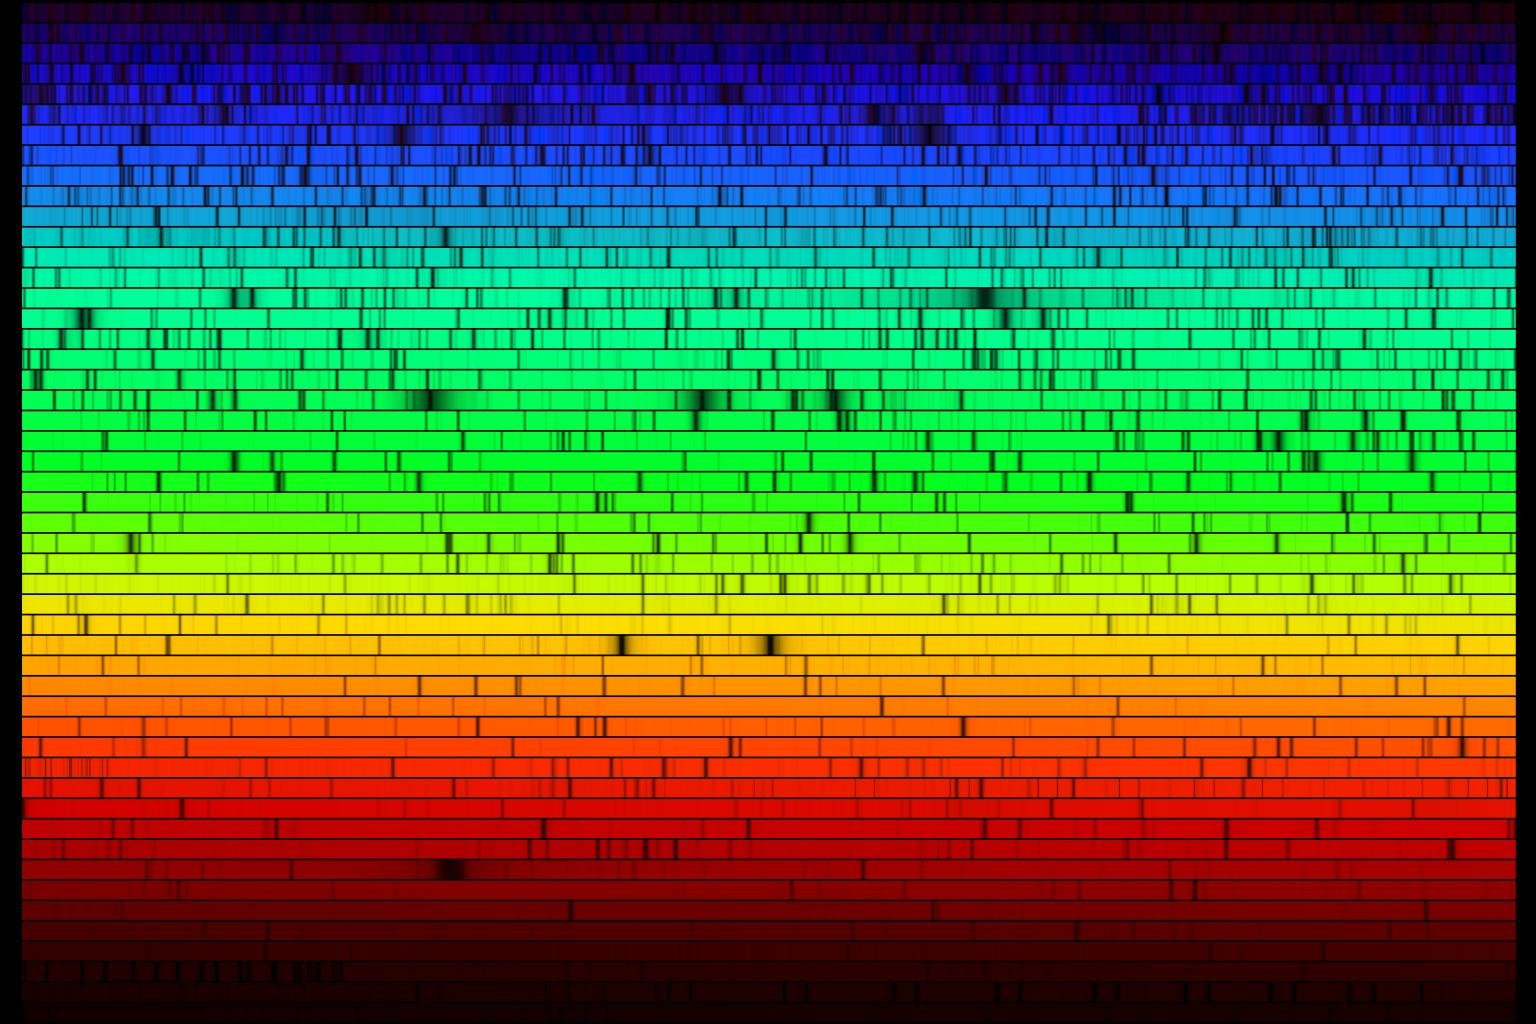
\includegraphics{'Figs/sun_spectrum.jpg'}
	\includegrpahics{'Figs/ fraunhofer-lines.gif'}
	\label{fig:fraunhofer}
	\caption{http://media.radiosai.org/journals/Vol_05/01JAN07/04-musings.htm}
\end{figure}


These lines are dark because they are absorption lines.
They are a result of the quantum mechanical effects of the electron energy shells around atoms and molecules.
In the case of the Sun, continuous white light spectrum is radiated from the photosphere, this light then interacts with the elements higher up in the atmosphere.
Upon incident with the atom or molecule, the exact wavelength of light which corresponds to the energy required to excite an electron from one energy level to another, is absorbed by the atom/molecule.
The direct result of this is that the wavelength absorbed in the energy transaction, is absent from the white light spectrum being emitted from the photosphere, and hence, appears as a dark line when observed from beyond the solar atmosphere. 

The field progressed and we began to fully understand the elements and electron transitions responsible for these abortion lines.
One of the most famous examples of these is the Balmer series, named for he man himself
This series is a set of 4 emission lines in the visible part of the Hydrogen spectrum, however, is specifically with respect to emission or absorption lines to and from energy level n = 2 as can be seen in \ref{fig:balmer}.

\begin{figure}
	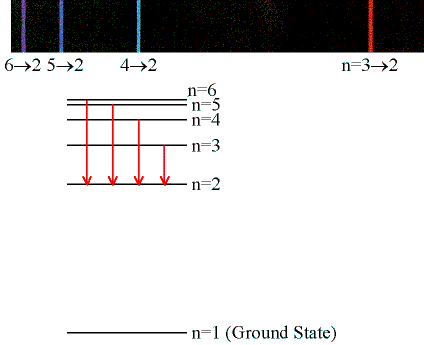
\includegraphics{'Figs/Balmer_series.gif'}
	\caption{http://www.daviddarling.info/encyclopedia/B/Balmer_series.html}
	\label{fig:balmer}
\end{figure}

Named after Johann Balmer, the transition from $n=3$ to $n=2$ is termed Hydrogen alpha (H$\alpha$), $n=4$ to $n=2$, Hyrdogen beta and so on for $n=5$ and $n=6$, gamma and delta respectively. 
However, while the concept of a simple 1-1 emission is clear, this does not always bear out in reality.
There can be environmental effects, such as temperature or magnetic field effecting the states of the energy level, which, can cause alteration of the wavelength of light emitted from the relaxation of the electron.
For instance, Hydrogen alpha is extremely useful for solar observation due to the high abundance of the atom in the atmosphere.
However, due to external factors influencing the energy levels, when we observe Hydrogen alpha, the deviation from the theoretical transition is sufficient to broaden the line to include both the upper photosphere and lower chromosphere.
Of course, Hydrogen does not just have transitions to the $n=2$, there are series associated with; $n=1$, Lyman, $n=3$, Paschen, Brackett details transitions to $n=4$ and Pfunf, $n=5$.

Clearly this methodology can be applied to all atoms and molecules that are in the solar atmosphere, allowing us to create a larger picture of the structure of the atmosphere.
We can do this by abundance and position, \emph{i.e.} there appears to be large amounts of a given transition line emission in this region and forming a structure by inspection.
As has already been said, we can associate certain transitions with various levels.
H$\alpha$ has already been discussed, moving up the atmosphere, He II $30.4$ \cite{Bazin2010} which is a Balmer-$\alpha$ transition, so $n=3$ to $n=2$, and has the same issue as H$\alpha$, in that it is extremely broad.
Calcium II and Silicon IV are both transition region, are utilised on-board the most recent space borne solar telescope, IRIS \citep{PereiraIRIS2014}. 
They are closely associated with the thin transition region, however, we do observe separate features not exclusively in the transition region.

Above the transition region Iron is bounteous, and so we have many emissions lines with which to examine the corona.
Fe VIII ($13.1$ nm), Fe IX ($17.1$ nm), Fe XII ($19.3$ nm), Fe XIV ($21.1$ nm), Fe XVI ($33.5$ nm) and Fe XVIII (9.4 nm) are all utilised on the spacecraft Solar Dynamic Observatory (SDO) with the instrument Atmospheric Imaging Assembly \cite{Schmelz2013}.
These multiple transition line from one atom are a result of the changing temperature, as it increases, the energy shells of the atoms alter, and so the various lines here apply to different temperatures.



% magnetic field recording
The energy shells of the atoms can also be effected by the environmental magnetic field, and as such we can find more out about the state of the plasma via spectroscopy as well.
The one of the effects which allows us to do this, is known as the Zeeman effect, in which, the magnetic field causes the energy levels to split based upon the spin of an electron, up or down.
The results in a splitting of what would be a single peak, into two, with the separation of the peak dependent of the size of the magnetic field present. 


\begin{figure}
	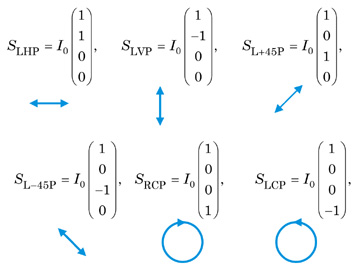
\includegraphics{Figs/stokes_params.jpg'}
	\label{stokes}
	\caption{https://spie.org/publications/fg05_p12-14_stokes_polarization_parameters. A Field guide to Polarisation.}
\end{figure}

A more suitable method by which we analyse the solar magnetic field is Stokes Polarisation Parameters.
In this method we test to what degree passing through a magnetic field has effected the electromagnetic radiation as it passes through.
In the method, the total intensity of an optical beam is defined to be a sum of three forms of polarisation, these 4 are refereed to as the polarisation parameters, I, Q, U and V.
I is raw intensity of the electromagnetic radiation, Q is the linear polarisation horizontally and vertically, U is also linearly polarized however is rotated $\pm45^\circ$ from Q and lastly V, which is polarised circularly, both left and right handed.
Using a combination of the 4 intensities it is possible to construct a vectorgram of the magnetic field and are utilised by the SDO instrument Helioseismic and Magnetic Imager (HMI) to examine features on disk.
These magnetograms are ineffective at the limb, which is a limitation of the method.
This is because a feature at the limb has no background light source to use as an origin to test the result of any polarisation. 

The vector magnetograms are used widely when studying active regions, due to the very high magnetic field strength.
They can track magnetic flux cancellation which regularly leads to the formation of other features, such as solar flares and CME's, due to the release of magnetic energy into the corona \cite{Welsch2006}.

We also observe the small magnetic bright points, which we have mentioned are observed in the photosphere and chromosphere \cite{SanchesAlmeida2010}.
They are an inherent part of what is known as the magnetic network which was visible in original measurements of the solar magnetic field over the boundaries of supergranular cells.
The magnetic field emerges from the supergranule boundaries as open magnetic field lines, extending up, into the chromosphere and above \citep{Hasan2005}.
Of course, the structure there for takes roughly the same form as the photospheric observations in G-Band,  however, with bright structures highlighting the supergranular lanes \ref{fig:mag_network}.
As a result, we have open magnetic field lines emerging with a canopy of closed magnetic field between the two boundaries.
A structure such as this can be an catalyst for physical processes such as reconnection.

It is within these regions that the magnetic bright points reside.
They appear as points of extreme intensities against the cool dark plasma of the interganular lanes, due to their intense $0.1$ T magnetic field strengths.
They are demonstrated to drift and move as the granules evolve \citep{Chitta2012} which has lead the community to suggest that these point could diffuse large amounts of heat into the solar atmosphere.

\begin{figure}
	\includegraphics{'Figs/magnetic_network_Ca_II.jpg'}
	\caption{http://science.nasa.gov/science-news/science-at-nasa/2008/02oct_oblatesun/}
	\label{fig:mag_network}
\end{figure}


\subsubsection{Coronagraphs}

Beyond $5 R_\circ$, the solar wind has become collisionless leading to minimal emissions as a result of the vastly decreased density.
Given this, we now change our approach to measure structures much further out in the corona and solar wind.
Currently, the only coronagraph still in operation is on-board the Solar Heliophysics Observatory (SoHO), the Large Angle and Spectrometric Coronagraph (LASCO). 
It is a white light detector which makes use of the effect known as Thompson Scattering which allows us to observe the particles which aren't directly emitting light off limb.
The effect entails a photon colliding with a particle, and colliding with a free charged particle in a classical sense, as opposed to a quantum interaction.
As a result of this interaction, the original photon remains unchanged in terms of energy and frequency, by this method, light from the Sun is scattered off the particles in the corona and it is this light that the coronograph detects.
In order to ensure that the detector is not washed out by the light from the Sun, ans occulting disc is essential to an operational coronagraph.


\subsection{Technology}

In the current solar observation climate, we have a wealth of information, coming from many different sources.
Understanding the functionality of these instruments in terms of the raw method is essential to rigorous science and accurate readings.

\subsubsection{Charge Coupled Devices (CCD's)}

CCD's are essential to current observational techniques and are utilised by almost every single solar mission.
They are an evolution of early photoelectric devices, which utilised the photoelectric effect, by which, a photon is incident upon a surface and an electron.
Cumulative photons exiting more electrons eventually produce a current sufficiently large to be detected.
The were known as photomultiplier devices, the drawback of which, was the restriction to a single detection per focal plane (pixel).
The primary issue with these dectectors is that they are extemely sensitive to background radiation, some on which is a result of the thermal emission from the detector.
Due to envirnomental effects cause inherent temperature of the detector to be non uniform as such the level of background can differ significantly too.
Of course, all of these effects can be corrected for, however, this will always increase the error value on the final result.

CCD's have since taken over the role which photomultipliers occupied.
Instead, CCD's are comprised of individual detectors all of high quantum efficiency arranged in a large grid, each element of which, is a single pixel.
An individual pixel keeps an electronic record of the photons striking it (summing them to an intensity).
Each pixel behaves as a potential well, trapping electrons produced as a result of the photoelectric events with the incoming photons.
The voltage resulting from the build up of electrons, is then recorded by the 

The particular advantage to a CCD is the linear response to the incoming photons \emph{i.e.} a one to one response to the incoming photons, giving extremely accurate results.
With respect to background noise and errors, the CCD is much easier to take regular dark current measurements (taking a reading with zero light coming in) and pixel to pixel variation is accounted for using flat fielding (exposing the grid to uniform field).
The gird of pixels approach also allows for much are flexibility in analysing data and correcting for the effects of events such as cosmic rays.
This is possible due to the ability to read these recordings into a computer.

\subsubsection{Ground Based telescopes}

Solar physics spent its early development being applied in ground bases solar telescopes, as has already been discussed, particularly in centres such as Royal Greenwich Observatory and Meudon Observatory in Paris.
In the modern era, the most powerful instruments, delivering high cadence and spatial resolution, are based on the ground.
Due to the challenges of observing on the ground, the location on these facilities is carefully chosen, regularly at high altitude, minimising disturbance of the signal by the atmosphere, and away from busy, polluting cities for the same reason.
The main advantages of ground based telescopes over space bourne, is that the instruments can be heavier and literally more extensive given that they do not need to be transported into space.

On La Palma in the canary islands, at $2360$ m altitude, the Swedish Solar Telescope is situated.
It utilises a $1.0$ m mirror in a refracting, vacuum solar telescope.
The vacuum is necessary due to the quantity of light the mirror reflects, causing heating which would disrupt the signal being transmitted down to a receiver.
The 'receiver' is what have become known as the optical bench, here the light beam is sent to one of several possible processing suites which are easily accessible to structure observations as needed.

SST has two such pipelines, one for the red end of the electromagnetic spectrum and another examining the blue end.
CRisp Imaging SpectroPolarimeter (CRISP), focuses on the red end of the visible spectrum, where as, the soon to be updated instrument, Chromis analyses the blue end.
The beam is split upon its arrival at the optical bench and sent to either of these instruments, however, before the beam reaches CRISP, there is a layer of correction known as adaptive optics.

Adaptive optics, corrects for atmospheric scintillation, aberration and stabilises image motion.
These cumulative effects results in an optical path difference of the light incident with the lens/mirror of the telescope.
Given this information, it is crucial to know the atmospheric physics overlying and surrounding the telescope.
It is for this reason, observatories such as the Big Bear Solar Observatory \citep{Cao2010} in Los Angeles, and the proposed new Chinese Giant Solar Telescopes \citep{Liu2014} are built on and by lakes, the reason being that the temperature will be lower, thus reducing heat haze, and therefore, atmospheric effects.
The primary atmospheric parameters influencing the set up of the adaptive optics are the Fried parameter (which measures the quality of optical transmission), the Greenwood frequency (the bandwidth required for optimal correction) and the atmospheric turbulence profile (which allows a calculation of the refractive index of the atmosphere) as shown in \cite{Rimmele2011}.

As a result of the above points, the images from the SST are extremely customisable.
They are usually returned as data cubes, with the dimensions of which are time, wavelength, x and y.
The resolution of these features are therefore changable dependant on the requirements of the observation.
Cadence can be as low as $2.5$ s, the spectral increment, $0.2$, and spatial resolution of $0.12$ arcsec.
A part of what makes this form of observation viable is the ability to directly download the received signal, which is a limitation of space borne instrumentation.
Given the possibilities of ground based observations, the method is popular, with the aforementioned Big Bear Observatory joined by a plethora of other facilities, Richard B. Dunne solar telescope (DST) in New Mexico, Mauna Loa Solar Observatory on Hawii, which will shortly be joined by the Daniel K. Inouye Solar telescope (DKIST).
DKIST promises to be the most powerful telescope ever created with a $4$ m mirror, enabling resolution of $10$ km per pixel and overcoming the quantity of photons issues at the limb for spectropolarimetry.



\subsubsection{Space Based telescopes}

Space bourne telescopes have a significant advantage over their ground based counterparts due to the nearly constant un-interrupted, view of the Sun without the atmospheric effects disturbing the signal.
As a result, the volume of space based instrumentation as grown exponentially since the early Skylab missions taking solar images from a low Earth orbit.

The first solar mission to move on from imagers on space stations was the Solar Heliospheric Observatory (SoHO).
Placed at the gravitationally stable lagrange point, L1, between the Sun and Earth, it affords constant viewing of the Sun.
It was one of the first missions to comprehensively over the entire solar environment, the instruments of which are described in \cite{StCyr}.
The science covers dopplergrams of the photosphere, EUV imaging of the chromosphere and out to LASCO, monitoring the solar wind.

Following SoHO, the Advanced Composition Explorer (ACE) \citep{Garrard1997} was placed near the L1 point as well.
It was launched in $1997$ with a much more specified goal of anaylsing the contents of the solar wind, extremely pertinent as the constituents and energy inherent in the solar wind can have extensive effects at Earth.
As a result of this, the scientific missions of ACE is heavily leant towards instrumentation which physically measures the energy and identity of a given particle.

The Solar Wind Ion Mass Spectrometer (SWICS) and Solar Wind Ion Composition Spectrometer (SWICS) are used to measure these properties.
SWICS was initially built for the ULYSSES \cite{Ulysses1992} mission which orbited the Sun in a novel slingshot orbit around jupiter, normal to the plane of orbit.

SWICS utilises a mechanical collimator to collect and direct the particles to an electrostatic deflecton array.
Whereupon, the incoming ions are deflected in accordance with the Lorentz force, $F_L = q(v x B)$.
Clearly therefore, particles incoming with higher velocities, or greater charge, will generate a larger Lorentz force, and therefore demonstrate a greater deflection when detected.
The detection is managed by a solid state detector, a semi conductor, which is applied in a similar way to CCD's.
When the particle interacts with the semiconductor, a 'charge carrier' is released.
This charge carrier is an electron currently residing in the valence band of the semi conductor, which, as a result of the particle interaction, is exited into the conduction band.
This leaves a 'hole' in the valence band, paired with the exited electron. 
The pair then migrates to opposite electrodes at either end of the semiconductor as a result of a background electric field, whereupon, they instigate a pulse which can be measured.
The amount of energy required to produce a given electron-hole pairs is known and so the particles can be inferred.

The results this instrument produced one of the most iconic set of readings in the modern era of Solar Physics.
As Ulysses completed its orbit, the radial velocity profile of the solar wind is found to vary over solar latitude.
At lower latitutes, the solar wind was found to be of the order $200$-$400$ kms$^{-1}$, before getting to higher latitudes and a distinct transition to much higher velocities.
At the time of this first orbit, the Sun was at a solar minimum, consequently, there were clear and distinct coronal holes and quiet Sun, matching with the fast and slow wind respectively.

\begin{figure}
	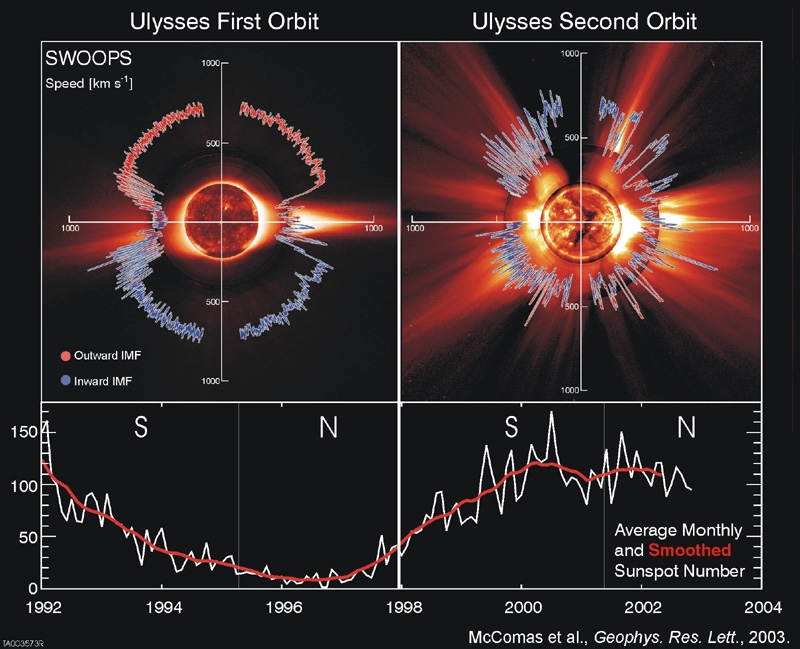
\includegraphics{Figs/ulysses_solar_wind.jpg}
	\caption{\cite{McComas2003}}
	\label{fig:ulysses_sw}
\end{figure}

The confirmation of this association between wind mode and magnetic environment came in the next orbit of Ulysses.
In this orbit, the Sun was at maximum, therefore, was almost entirely constituted of quiet Sun magnetic environments.
During this orbit, the solar wind was found to be uniformly chaotic.
Velocities are found to climb as high as those found in a fast solar wind mode, however it is not the uniformly distributed fast mode emitted from the coronal holes, as evident in the solar minima readings.

Given that we now know that the solar wind and corona have significant reach and influence, a new mission was designed and initiated, the Transition Region and Coronal Explorer (TRACE) \cite{Gaeng1998}.
As the name suggests, this instrument was designed with the specific intention on investigating the higher reaches of the solar atmosphere.
Specifically, the aim of the mission was to investigate the three dimensional structure of the low plasma beta atmosphere.
TRACE is a uniquely designed telescope, following the popular Cassegrain design, in which, the primary mirror is divided up into 4 quadrants with separate coatings in order to filter the incoming light.
This method allows simple and efficient image co-aligning.
Given that TRACE was to observe the high atmosphere, Extreme Ultra Violet lines (with the rest of the EM spectrum filtered at entrance to the detector) were selected for the imaging instruments, Fe IX $17.1$ nm, Fe XII $19.5$ nm and Fe XV $28.4$ nm.




The Japanese Aerospace Exploration Agency have organised several solar missions, Solar-A, renamed Yohkoh, \cite{Tsuneta1992} upon its successful launch and commencement of observations, pre-dates SoHO.
It covered soft and hard X-Ray ranges and spectrometers covering, specifically, the coronal Iron lines and a wide band spectrometer. 
Yohkoh was particularly successful with respect to the detection of high energy events producing large amounts of energy and X-ray emission, such as coronal jets and solar flares.
Building on the success of Yohkoh, a new mission was planned, sequentially named Solar-B and later to be renamed Hinode, sunrise in english, upon its successful launch and is presented in \cite{Kosugi2007}.
 
Hinodes launch in 2007 signified a significant move forward in space based solar observations, building from what was successful in Yohkoh.
The mission introduced small wavelength increment spectroscopy to space based missions.
The EUV Imaging Spectrometer (EIS) is designed to examine the chromospheric atmosphere using two specific imaging techniques.
It is extremely flexible with 4 slit or slot positions, $1"$ pixel slit, $2"$ pixel slit, $40"$ pixel slot and $266"$ and two different modes spectroscopy.

The spectroscopy mode 
 


Possibly the most adventurous mission to probe the solar environment is the STEREO mission (Solar TErrestrial RElations Observatory, quoted this way round due to the clear bacronym) presented in \cite{Kaiser2008}.
As is suggested by the name of this mission, the primary focus was to form a more comprehensive picture of the solar atmosphere, by positioning two satellites in such an orientation to build a three dimensional picture.
Consequently, two identical satellites were launched into \emph{solar} orbits, ahead and behind the orbit.
There is an inherent differential in the angular velocity of the spacecraft, in order to move the spacecraft ever further around the orbit at approximately $45^\circ$ per year.
The primary objective of this stage of the mission was to obtain the optimal angle to produce three dimensional images of the Sun using a tomographic technique.

Given that STEREO was designed to give varying angles of the solar-earth  enviroment, the instruments on the mission are tailored to this need.
SECCHI is a suite of 5 imagers, utilising white light chronographs, an extreme ultra violet imager and two wide angle Heliospheic Imagers (HI) designed to track CME's to $1$ AU.
IMPACT detects solar wind electrons and in situ solar wind magnetic field strength and vector, while PLASTIC measures composition of heavy ions, alpha particles and protons. 
Given the instumentation, STEREO is used extensively by space weather forecasters at NOAA, which, will increasingly become and essential part of our lives.

Building on all of the above missions, the Solar Dynamic Observatory (SDO) mission begun in 2010 \cite{Kaiser2008}.
The instruments are developments of concepts used on previous missions but expanding them to allow constant viewing of the entire solar disk.
Consequently all instruments on SDO view the full solar disk, at all times, maintaining the same temporal cadence. 
Therefore, the SDO mission produces significantly more raw data than any previous, from an purely engineering standpoint, the instruments were carefully selected to facilitate the downloading of the data.
As such, SDO has three scientific aims; the Helioseismic and magnetic Imager (HmI) examining the solar variability and finer scale structure of the solar magnetic field; Extreme Ultraviolet Variability Experiment (EVE) measured the total solar irradiance in the Extreme Ultra Violet section of the spectrum and the Atmospheric Imaging Assembly (AIA) investigating the upper chromosphere and corona.

AIA's imaging suite provides full disk images in $4096 \times 4096$ resolution and most importantly at $12$ second cadence.
However, its distinguishing feature is the array of wavelengths analysing the atmosphere \cite{AIAspec} associated with various temperatures equivalent to the appropriate electron transitions.
The instrument ranges through $170$, $30.4$, $160$, $17.1$, $19.3$, $21.1$, $33.5$, $9.4$ and $13.1$ nm providing a temperature range of $5000$ K to $1.6 \times 10^7$ K.




\section{Plasma behaviour}

Stars are incredibly unique features, their behaviour is entirely unlike any planetary body, and has already been discussed, their inherent magnetic field makes their structure extremely complex.All of these affects can be traced back to the fact that the Sun consists of gas kept at high temperature and pressure, which causes it to form the $4^{th}$ state of matter, plasma.
Plasma is defined as a gas in which the molecules reached an energy level that cause them to eject their outermost electrons and become Ions, causing the gas to be a neutral mixture of charged Ions and free electrons (produced from ionising the molecules).
It can be formed in several situations, such as a discharge of current from the atmosphere to the ground, manifesting as lightening as the propagating current ionises the air.

The motion and behaviour of a plasma can be defined on small scales but 3 factors; The plasma approximation, bulk interaction and the plasma frequency.
The plasma approximation states that the particles must be close enough together such that any given particle must influence all particles within the Debye screening length.
The length is dependant on the permittivity of free space, the Boltzmann constant, electron charge, temperatures of the Ions and electrons, density of electrons and density of an atomic species.

\begin{equation}
	\lambda_D = \sqrt{(\epsilon_0\kappa_BT_e)/(n_eq_e^2)}
\end{equation}

Bulk interaction refers to the statement that the Debye screening length is small compared to the overall scale of the plasma, this implies that the motion of the interior guides the characteristic behaviour, rather than motion at the edges.
Lastly the plasma frequency refers to the oscillation of the elections within the plasma, which is valid if this frequency is higher than the collions between electrons and neutrals.
In this case, the electrostatic interactions dominate over the standard, gas-like behaviour we would otherwise see.
Of course, the case where all the molecules or atoms are ionised is the ideal case, however, in nature this is not always true.
The degree of the ionisation is defined in terms of the ratio of ions to electrons, $\alpha = n_i/{n_i + n_n}$ where $i$ is the number density of ions and $n$ for neutrals.

As is evident from the Debye screening length, the temperture of the plasma, can have a dominating effect on the characteristics of the plasma.
The temperature is a measure of the thermal kinetic energy of the plasma, clearly higher kinetic energy therefore equates to a higher temperature of the plasma.
However, electrons will reach a thermal equillibrium significantly faster than the ions and neutrals, in which situation the plasma will have two, or even three, populations.
In the case where the plasmas electrons and ions in thermal equilibrium with the neutrals the plasma is termed, shockingly enough, thermal.
In nonthermal plasmas, the electrons, whose temperatures raise quicker, will be at a higher temperature than the heavier ions and neutrals.
The degree of ionisation of the plasma that results a thermal equilibrium us given by the following;

\begin{equation}
	x^2/{x - 1} = (2\pim_e)^{3/2}/h^3 (\kappa_BT)^{5/2}/p_{gas} exp(-{\chi/\kappa_BT}), \cite{Saha1920}
\end{equation}

Where $p_{gas}$ is the gas pressure, $m_e$ is the mass of the electron amd $\chi$ is the ionisation energy.
This form of the Saha ionisation equation will hold for Hydrogen, however does not take into account multiple ionisation processes, as would be the case for a more complex atom or molecules.
The result of this is that degree of ionisation in a gas will increase with increases in temperature.
It therefore follows that not all plasmas are fully ionised, at lower temperatures, the heavier elements won't gain enough energy to ionise, sometimes despite the fact that the electrons are orders of magnitude higher in temperature.

Given that plasma behaves differently, we therefore need a set of laws to define how the plasma behaves on scales such as those applicable on the Sun and in the atmosphere.


\subsection{MHD}

Magnetohydrodynamics are the set of laws by which we describe the motion of plasma on scales.
They were derived by \cite{Alfven1942}, an achievement for which, Alfv{\'e}n was awarded the nobel prize.	
The rules set up are a combination of the gas pressure equations and Maxwell's laws of electrodynamics, so let us now examine this relationship.

When considering a plasma, it is important to remember that while the total charge of the plasma will be quasi-neutral, the ions and electrons which constitute the mixture still carry charge.
Consequently, motions in the plasma will cause the charges to have a change in velocity.
In accordance with Farady's law, a moving charge will cause a magnetic field to be induced and Ohms' law will also become a factor with charges moving through a magnetic field.
As such, this can be an extremely complex problem, let us begin our discussion with Maxwell's equations;

\begin{equation}
	\divv \times \mb{E} = -\pd{\mb{B}}{t} & & \textnormal{Faradys}
	
	\divv \times \mu_0\mb{j} + \frac{1}{c^2}\pd{\mb{E}}{t} & & \textnormal{Amp{\`e}re}
	
	\divv{\mb{E}} = \frac{\tau}{\epsilon_0} & & \textnormal{Gauss'}
	
	\divv{\mb{B} = 0} & & \textnormal{Gauss' law of magnetism}
\end{equation}

where $\mb{E}$ is the electric field stength, $\mb{B}$ the magnetic field, $t$ is time, $c^2 = (\epsilon_0\mu_0)^{-1}$,$\epsilon_0$ is the vacuum permittivity, $\mu_0$ is the permeability of free space, $\mb{j}$ is the current density and $\tau$ is the charge density.
Faraday's law describes how a changing magnetic field would induced an electric field, hence it is also known as the Induction equation.
Amp{\`e}re's law describes the manner in which the magnetic field integrated around a closed loop, related to the electric current passing through said loop.
Gauss' law for magnetism is also known as the Solenoidal condition and states that no magnetic monopoles exist and the eponymous law describes the resulting electric field caused by an electric charge.

The second `half' of the magnetohydrodynamic equations are the laws for gas dynamics, expressed in terms of the partial derivatives;

\begin{equation}
	\pd{\rho}{t} + \del \cdot (\rho\mb{v}) = 0 & & \textnormal{Equation of mass conservation}
	
	\pd{p}{t} + \mb{v\cdot}\divv{p} + \gamma p\divv{\cdot}\mb{v} = 0 & & \textnormal{Conservation of entropy}
\end{equation}

in Eulerian time-dervative reference frame, evaluated for a fixed position within the fluid.
In the case of these two sets of equations, there is currently no link other than the velocity vector, $\mb{v}(\mb{r},t)$ which can be introduced through the equation of motion for a fluid element.
The equation for the motion of the fluid element is derived from the rate of change of momentum equations 

\begin{equation}
	$\frac{d}{dt}\int_{V}^{}dV\rho\mb{v} = \int_{V}^{}dV\rho\td{\mb{v}}{t} = rate of change of momentum$
\end{equation}

In this case the rate if change of momentum will equal the net force on the fluid element, in accordance with newtons second law, therefore;

\begin{equation}
	\rho \td{\mb{v}}{f} = \rho\mb{g} + \divv{\cdot}[X]
\end{equation}

where X is the total of all forces exerted on the fluid element. 
Therefore the equation which will incorporate all of these terms and calculate the acceletation on a fluid element is:

\begin{equation}
	\rho \td{\mb{v}}{t} = \mb{F} \equiv -\divv{p} + \rho\mb{g} + \mb{j} \times \mb{B + \tau\mb{E}} 
\end{equation}

As we are currently assuming that we have a totally ionised fluid, therefore the electric field is defined as

\begin{equation}
	\mb{E}' \equiv \mb{E} + \mb{v} \times \mb{B} = 0
\end{equation}

and therefore, $\mb{E}'$ in a co-moving frame will vanish.
The last assumption we need to make, is that the velocity of the plasma is not relativistic $v \ll c$.

This allows us to make some assertions as to the scale of the terms in Amp{\`e}re's equation, the length scales of $l_0$ and $t_0$ are shown such that $v = l_0/t_0$.
This means we can negelect the displacement current from Amp{\`e}re's and define the current $\mb{j}$ purely in terms of \mb{B}:

\begin{equation}
	\mb{j} = \frac{1}{\mu_0}\del \times \mb{B}
\end{equation}

As a result of which, we can neglect the effects of space charge on the plasma.
Additionally, the non-relativistic assumption means that we can also make a simplification to the acceleration of a fluid element equation as the electrostatic acceleration is small, as well, Gauss' can be dropped through lack of need.
As such the electric field can expressed merely in terms of the velcoity and magneticfield vectors:

\begin{equation}
	\mb{E} = -\mb{v} \times \mb{B}
\end{equation}

But applying the above assumptions, and substituteing in for $\mb{E}$ and $\mb{j}$, we obtain the basic equations of ideal magnetohydrodynamics (MHD).

\begin{equation}
	\pd{\rho}{t} + \del\cdot(\rho\mb{v}) = 0
	
	\rho(\pd{\mb{v}}{t} + \mb{v}\cdot\divv{\mb{v}}) + \divv{p} - \rho\mb{g} - \frac{1}{\mu_0}(\del \times \mb{B}) \times \mb{B} = 0
	
	\pd{p}{t} + \mb{v}\cdot\divv{p} + \gammap\del\cdot\mb{v} = 0
	
	\pd{\mb{B}}{t} - \del \times (\mb{v} \times \mb{B}) = 0
	
	\del\cdot\mb{B}
\end{equation}

These equations are therefore applicable to the case where; 1) the plasma is strongly collisional, such that the time scale of the collision between the particles is much smaller that the characteristic time scales of the entire system.
2) The resistivity of these collisions is small \emph{i.e.} the magnetic diffusion time scale much be longer than any other process occurring within the plasma.
3) The time scale must be greater than that of the kinetic processes occuring within the plasma, such as ion gyration, Landau damping and length scales longer than the ion skin depth and Larmor radius.

By making choices with respect to the units for length, mass and time, the MHD equations can be made dimensionless.
A typical length scale can be chosen such as $l_0$ to be something sensible and $\rho_0$ and $B_0$ are chosen from a representative point in the plasma and the time unit can be inffered from a basic speed of the plasma, \emph{e.g.} the sound speed or Alf{\`e}n speed.

\begin{equation}
	v_0 \equiv v_{A,0} \equiv \frac{B_0}{\sqrt{\mu_0\rho_0}} \textnormal{which leads to} t_0 \equiv \frac{l_0}{v_0} 
\end{equation}

The density, velocity, magnetic field etc. are then used to define new dimensionless parameters and substituted back into the MHD equations, which remain unchanged but npow a have an operator for these variables instead of the variable themselves.
the crucial outcome here is that equations are not dependent on the size of the plasma evaluated, the magnetic field strength, the density or the time scale.
After scaling $l_0$, $B_0$ and $t_0$, the pressure term becomes of vital importance and is linked to the ratio between the kinetic pressure of the plasma and magnetic pressure.
This ratio is commonly referred to as the plasma beta, and is defined:

\begin{equation}
	\beta \equiv \frac{2\mu_0p_0}{B_0^2}
\end{equation} 

This is and extremely useful flag when considering the behaviour of a plasma at a less precise level, as it indicates the forces dominant in a region.
If $\beta \gg 1$ the pressure terms are dominant, meaning that the kinetic motions of the plasma will determine its overall behaviour, such as in the photosphere and below.
Whereas, in the chromosphere and upwards, the balance more favours the magnetic field and the gas movement is determined by magnetic effects.
Which leads us to another important result of ideal MHD, the frozen in condition.





\subsection{Reconnection}

\section{Jet and Macrospicules}

The appearance of thin, explosive features with a relatively short lifespan has always been a part of solar physics.
Spicules were first observed in 1877 by a vatican observer, Angelo Secchi.
This was aided by their sheer ubiquity, they were distinctly visible at the solar limb nearly all the time.
However the larger scale, more infrequent jets are more difficult to observe, particularly with early solar observations.

\subsection{The ejecta zoo}

The wide variety of jets and jet like feature 
Jets and jet like features are observed throughout the solar atmosphere, and as such a review of the topic is in order.
As has already been discussed, spicules are the smallest jets formed in the solar atmosphere, 
most easily observed at the limb, they are long thin structure appearing brightly at the solar limb \citep{Beckers1972}.
Spicules are found in the chromosphere, regularly observed in the H$\alpha$, He II $30.4$ nm, Ca II and Si IV.
Work by \cite{DePontieu} divided spicules into two populations, Type-1 and Type-2, with Type-1 being long lived and Type-2 having distinctly shorter lifetimes, but however are significantly more explosive and grow to much higher lengths .
Type-1 spicules have an uprising speed of approximately $20$ kms$^{-1}$ and extend to $1$ Mm in height, whereas the Type-2 spicules have been shown to extend approximately $5$ Mm into the atmosphere and last for an average of $10$ minutes.
The most comprehensive difference between the two is in the overall evolution of the feature.
Type 1 spicules are observed to have a parabolic evolution \emph{i.e.} their tip traced out a ballistic arc when plotted against time.
Conversely, Type II spicules are observed to dissipate or vanish as they evolve, and are primarily observed in the quiet Sun and coronal holes, Type I develop in active regions, as such, Type II are far more numerous when recorded in a study such as \cite{Pereira2012}.

\begin{figure}
	\includegaphics{'Figs/spicules_at_limb.jpg'}
	\caption{http://www.nasa.gov/sites/default/files/images/751917main_highres4_full.jpg Spicules as observed by Hinode}
\end{figure}

Spicules are visible on the disk as well, however, on disk we see dark thin structures against the bright lower chromosphere, these were initially named mottles and fibris, however have since been inherently linked with spicules, see \cite{DePointeu2007MF}.

Since these initial propositions, however, there has been doubt cast as to whether this is the case or not. 
Cite Zhang 2010 found no statistical separation of populations within spicules and recent publications but the original authors have shown that Type-2 spicules disappear from Ca II and reappear in the hotter Si IV and Mg II lines \citep{Pereira2014}.
This would imply that spicules are heating as they accelerate through the atmosphere, whether this is because the underlying formation mechanism is different or there is sufficient energy in the initialisation of the spicule to cause heating as they propagate through the atmosphere, has yet to be made clear.

The formation of spicules is still a matter of much debate given our currently limited ability to examine small scales in current observations. 
However, when observations are unable to provide explict results, numerical and analytic approaches are utilised to fill in the gaps.
\cite{DePointeu2004} outline a mechanism for the formation of spicules which originates in the photosphere.
P-mode oscillations cannot pass through the photosphere due to the minimum temperature, however, evanescence allows the waves to propogate into the higher atmosphere, where higher temperatures allow propagation to restart.
Also essential to this model is the inclination of the native magnetic field.
The authors report that the inclined field, vastly increases the likelihood of waves tunneling through the atmosphere. 
In the lower density solar atmosphere causes the photospheric velocity generated by the p-modes to leak into the atmosphere and steepen into shocks, which leave and oscillating wake in the chromosphere, the spicule.

However this is only one of many competing theories, \cite{Takeuchi2001}, demonstrate a magnetic reconnection model driving formation of spicules, whereas \cite{Martinez2011} formed a $3$ dimensional model utilising the Lorentz force to push plasma across the solar surface until it meets vertical magnetic field which forces the plasma upwards.
\cite{Hollweg1982} demonstrate a quasi-impulsive source in the photosphere is capable of generating a chain of rebound shocks in the chromosphere, causing the formation of a spicule.

A particularly pertinent model is proposed by \cite{Moore2011spic_recon}, in which magnetic reconnection is instigated by granule sized 'magnetic bubbles'.
This is applicable, as spicules are generally observed to form on the intergranular lanes.
The authors propose that Type 2 spicules are an analogue for X-ray jets (more on which later).
In this scenario, magnetic bipoles emerge from the photosphere which then interacts with the ambient field of the lower chromosphere, forming a raft of reconnection external to the bipole.
During this reconnection, the interior of the bipole remains inert while the outer most sections of the structure, 'sling shot snapping' of the magnetic reconnected field lines produce; an upward jet (Type II spicule), Alfven waves propagating up the ambient magnetic field lines and a fast MHD wave upwards across the magntic field.

The advantages of this scenario for connection is that the environment which generates these spicules, is eminently reproducible throughout the solar surface.
The scenario here is particularly convenient as it also answers questions with respect to heating of the solar atmosphere.
As a result of the 'canopy region' that forms over the granules reconnecting with the more open magnetic fields higher in the atmosphere, causing shocks and waves to propagate upwards.
The dissipation of the energy within these disturbances, has been proposed on numerous occasions to be the central source of heating of the corona.  

What becomes evident, after all of these models are formed, none of them generate both Type I and type II spicules, therefore it is likely that they are indeed two separate features.


Throughout the solar atmosphere, we observe much larger jet-like features than spicules.
They have been observed extensively, and not solely in the chromosphere.
The first observations of more large scale jet were undertaken using the Soft X-Ray telescope on board Yohkoh \citep{Tsuneta1991}.
\cite{Shimojo1996} undertook the first statistical study of jets, finding a nice round $100$ examples to study.
With any study looking for specific features, the authors utilised the following selection criteria; 1) That the plasma is collimated and that the movement of the feature was in the direction of the collimation, 2) The aspect ratio of length to width is greater than $3$ and 3) The time between the pre-jet image and the image in which the jet first appears is less than an hour.
These are an excellent example of selection criteria which aide in forming the search, however, are vague enough not to introduce bias into the sample.

The authors find that the jets are primarily formed with a microflare/sub flares at the base/footpoints (the terms are used interchangeably in literature).
They find their lengths to be of the order $10$ - $400$ Mm and widths are of the order $5$-$500$ Mm.
Velocities along the direction of collimation we observed to range between $10$ and $1000$ kms$^{-1}$, averaging at approximately $200$ kms$^{-1}$ lifetimes extending to $10$ hours.
In terms of physical evolution of their shapes, the authors find that $76\%$ of the jets demonstrated converging shapes, \emph{i.e.} the width of the jet would be constant over its evolution or decreasing with distance from the footpoint. The constant form were found to come from a wide variety of energy sources, whereas the converging form, explicitly formed from energetic points. 
This work has formed the basis of much of the study of jet phenomena, however, this is merely an exploratory study around which future studies have explored.

% possibly more required here

What has become known as the standard model for the formation of solar jets is demonstrated  by \cite{Shibata1992}.
Within this paper, the authors use the Soft X-Ray telescope on Yohkoh to examine $20$ jets, and present their spatial properties, very similar to those of \cite{Shimojo1996}, however, the authors go on to describe a possible formation schematic.
The model is based upon the flux emergence from the lower solar atmosphere, and is backed up by data in the Solar Geophysical Data.
The authors demonstrate that the observations reveal a void at the jet base, similar in appearance to voids observed in reconnection driven events such as flares and CME's.
The authors proposed that the jets are based in the chromosphere based on an inspection of the emission measure, consequently it is likely that the mass is from the chromosphere.
The authors propose that the undulating and meandering shape of the jet lends itself to a helically twisting magnetic structure, suggesting that the jet itself emanates from a relaxation of the magentic field along a global flux tube \cite{Shibata1986}.
Such a reconnection event between twisted and untwisted magnetic field, would be capable of producing a jet of this size, lifetime, and more importantly, velocity.

This model for the standard jet requires that there be open magnetic field lines, and a smaller scale, twisted, emgering flux loop to rise from the lower atmosphere in order to initiate a reconnection event.
As a result of the reconnection event, material in the emerging loop is than transfered into the open magnetic field lines, 'sling shotting' around the loop it as formerly a part of and up the open field lines, thus revealing the collimated beam of plasma.
The mechanism highlighted in this particular model produces exclusively narrow jets, a couple of mega meters in width.
It also results in the dissipation of large amounts of energy which manifests as brightenings in may observations.
From the source of the reconnection, energised plasma then dissipates down the loops highlighting the entire feature.
The visual effect of the long collimated beam/plasma spire and the newly brightened loop of plasma, reveals an 'inverted - Y' shape or Eiffel tower like structure, similar to the 'cusp' shape observed in significantly larger features high in the corona round streamers and flares \cite{Vourlidas2006}.
These terms have gained common usage in literature and will be used hereafter. 

An excellent example of this type of formation is demonstrated in \cite{Nishizuka2011}.
Within this work, the authors demonstrate what is refereed to as an Anemone jet, so called as the dome like bipole magnetic bubble, may be viewed as a feature similar to the sea creature.
The model they build as a result of this is in three dimensions, consequently, the small scale loops of the standard model could be projected into $3$D as an anemone-like shape.
The authors observed the jet in Ca II, it formed along an inclined line approximately $45^\circ$ away from normal, in the inverted-y format.
With the jet forming in Ca II, we can conclude that this particular jet is formed in the upper chromosphere, with this particular jet the authors observe the formation loop itself.
The jet feature is found to extend $14$ Mm into the atmosphere and its width, $6$ Mm, with maximum velocity observed at $100$ kms$^{-1}$, however, $10$ minutes into the evolution of the jet, contrary to what you might expect.

The standard jet model accurately describes a prominent section of the jet population, however, those which it does not cover is highlighted in \cite{Moore2010}.
The specific example that the standard jet model does not cover is the case where the width of the jet is more than that predicted by the standard model.
\cite{Moore2010} utilise Hinode/XRT to look for X-ray jets occuring in the polar coronal holes, and where possible the authors observed the same features in EUVI as well.

The initial magnetic field topology is largely similar to that of the standard jet, a small scale loop with open magnetic field extending upwards.
The difference in these models is that the emerging bipole arch in the case of the standard jet, remains untwisted and without shear.
In the case of blowout jets, this arch/loop is sufficiently twisted and sheared that it can drive an explosive eruption.
In terms of the physical evolution, there is no difference between the two until the emerging flux element triggers a reconnection burst at the boundary between said emerging flux and the open magnetic field lines.

The authors then go on to suggest two resolutions to the reconnection event; that the boundary becomes unstable on its own, and consequently reconnection begins on its own.
This results in beakout reconnection, expelling the loops outer magnetic field, which lifts the restriction on sheared flux lower in the system; consequently allowing the core of the emerging flux to erupt upwards. 
This forms a chain event, with emerging core events causing more reconnection and consequent releases and so on, similar to \cite{Antiochos1998}.
The second permutation, is that the sheared core, begins to erupt before any reconnection takes place at the boundary.
In this scenario, an instability in the emerging bipole causes the previously stable core to begin emerging.
As a result, magnetic pressure at the boundary current sheet between the loop and open magnetic loop, eventually triggering breakout reconnection.

This work clearly has impact on the current relationships between the various jets of scales larger than spicules (which clearly are their own feature.)
The authors propose that the blowout jets correspond to the macrospicule features in the chromosphere, more on which later.
As for implications with respect to the division of standard and blowout jets, observations of the formation mechanism would clarify the feature.
Standard jets would have large originating loop spanning approximately $20$ Mm or not visible at temperatures lower than  $10^6$ K.
Whereas, blowout jets need to produce strong signals in H$\alpha$ and He $30.4$, due to the cooler plasma thrown upwards from the unstable magnetic bipole emerging.

One of the most comprehensive sets of jet observations is undertaken by \cite{Majarska2011}, in which, the authors observe a jet in an equatorial coronal hole.
Utilising, SUMER on SoHO, EIS and XRT on Hinode and the EUVI instruments on the STEREO A and B.
The authors find that the jet can be heated my microflares at the moment of reconnection, rising the temperature up to $12$ MK.
This was obtained using a DEM technique integrating the emission from a range of spectral lines to estimate the temperature, and the density was approximated at $4 \times 10^9$ cm$^{-3}$ using a similar technique.
http://www.aanda.org/articles/aa/pdf/2011/02/aa15269-10.pdf
% more here?

% This section may need to go else where
What becomes clear is that these large scale jets can only be trigger by explosive reconnection events, therefore understanding this mechanism is essential to out understanding of solar jets.
\cite{Archontis2005} demonstrate the mechanism governing the rules of this interaction.
Essential to any useful numerical simulation is a reasonable set of initial conditions which succinctly defines the environment of the feature.
In the case of the authors define a background stratification of the gases \emph{i.e.} non-magnetic; a horizontal magnetic tube which is inherently twisted and buoyant; a uniform horizontal magnetic field in the corona and transition region.
The exact parameters of the background stratification and magnetic tube are defined in \cite{Fan2001}.

The 'box' which contains the simulation, incorporates the top of the solar interior, to a depth of $3.74$ Mm from the photosphere, the bottom of which is set as 0 and extends to $1.7$ Mm, represented as an isothermal zone.
Over the next $3.7$ Mm of height, the temperature rises steeply mimicking the effects of the transitions region.
Lastly there is a second isothermal region which extends to a distance of $11.9$ Mm from the photosphere.

The horizontal magnetic tube, which will eventuality emerge through the atmosphere, field is a Gaussian distribution, symmetrical about the longitude and the field lines are helically twisted in a uniform fashion around the central axis.
The issue with this set-up is that in the case of kink-unstable cases, the model will supress onset of internal current sheets. 
The stratification of the background gas is applied to the tube by applying a perturbation in the gas pressure, such that the stress tensor has zero divergence and vanished in the case $r/R \gg 1$.

The gas density was within the tube is not however symmetrical about the 'latitudinal' direction.
In order to illicit a rising response from the magnetic tube, the centre region is given a density $1/\beta$ lower than the region around it as a result of the density perturbations.
The causes the tube to undertake a transformation into the characteristic $\Omega$-loop shape which emerges into the atmosphere.
Lastly the coronal magnetic field is straight horizontal and space filling, it is highest in the corona and reduces through the transition region and photosphere.

The simulations show that reconnection is immediate when the two flux objects come into contact, with the current sheet forming between them aligned with the direction of the axis of the flux tube.
This is greatly accentuated by the horizontal field above, however, once the flux tube magnetic field and the coronal magnetic field are equal, the reconnection lessens to a smaller constant volume. 
At the current sheet region, the magnetic field lines of the flux tube is anti parallel to those of the coronal magnetic.
As the outer regions of the flux tube are cancelled away, however, the field in the tube rotates away from anti parallel as is the nature of a twisted flux tubes.
Hence the boundary behaviour changed from the current sheet to a tangential discontinuity and finally to a rotational one.

The authors present evidence of continuous reconnection at the boundary, the work demonstrates that the first line undergoing reconnection, instead of passing through the boundary of the other end of the flux tube, it passes directly into the coronal region.
The end point of the field line is then travelling at a new velocity, different to that of the local plasma at the new boundary.
The implication of this is that field lines at he boundary between the two regions, undergoes continuous reconnection, however, once it has passed though integrates into the coronal plasma.
The helically twisted nature of the flux tube, allows for multiple reconnection instances.
Consider looking at the end of the flux rope as a cross sectional area, when the reconnection occurs, a magnetic field line reconnects with the magnetic field in the corona, and is draw straight into the corona while the rest of the line remains attached to the flux tube instead of the entire line detaching.
As a result of this gradual detachment and the twist, the end of the field line traces out a circular motion in our cross section; first reaching into the coronal then being draw around and through the transition region, underneath the tube, back through the atmosphere and into the corona before lastly returning to the solar interior.

Importantly, high speed jets are observed at the reconnection site, the plasma blasts through the current sheet before interacting with the higher pressure gas above it, therefore guiding it along the inclined magnetic field lines.
In this case, the jets are observed as curves, and as such, disappear when observed on a horizontal plane.
The authors then relate this th H$\alpha$ filaments and brightenings or jets in solt X-ray, the energy required to cause brightening is X-ray would be supplied by the interaction of these two flux systems, they also calculate a temperature increase to $10^7$ K.

Recent studies have demonstrated the prevalence of smaller scale jets at the magnetic network boundaries.
\cite{Tian02014}, and later built on by \cite{Nagrang2016}, highlighted these features using the most recent addition to the solar observational tools available to us.
The network boundaries are regions where there is a great deal of magnetic complexity and strong field values, and almost certainly a large amount of reconnection will be apparent.
These strong fluxes emminate from the boundaries of the granules, and therefore, convection cells.
The evidence of this is apparent when imaging the transition region, the bright lanes approximately $20$ Mm in size, it is possible that these regions appear bright in the transition region due to the heating as a result of reconnective events. 

The authors find explosive upflows in the direct images from IRIS with velocities of $80-250$ kms$^{-1}$ and using the superior resolution of IRIS idenify jet-like features developing from the bright networks.
These jets are long and thin features,$4$-$15$ Mm in length and ~$0.3$ Mm in width, and demonstrate just upflows, no downflows a evident.
These events are extremely shortlived, with lifetimes measured at $20$-$80$ seconds, however, there is recurrence observed with jets forming repeatedly in the same location, with time scales in the range $2$-$15$ mins.

Observations using the spectral lines leads them to the conclusion that the jet like features heat to temperatures of the order $10^5$ kms$^{-1}$, in this case the temperature of Si IV $139.377$ nm.
This Si IV line also allows an analysis of the line broadening which could possibly be due to the field aligned jets, as is proposed in \cite{Archontis2005}.
The jets are also shown to be an intermittent but effectively continuous source of mass, and therefore energy, into the solar wind.
As such, the author propse these network jets as new mechanisms for generating the solar wind.

Chromospheric Jets?




\subsection{Macrospicules}


The subject of this thesis is a clarification of the classification of macrospicules. 
They are features not dissimilar to jets, however they have been distinguished from the population of jets in the current literature, which will now be discussed below.

Macrospicules were first reported by \cite{Bohlin1975}, utilising the SkyLab mission.
This was undertaken using $30.4$ nm instrument making observations of the polar coronal holes.
The initial images were taken as raw light through particular filters over the lens, the images were also over exposed in order accentuate the appearance of the solar limb.
The authors found that the newly named macrospicule was visible in He II $30.4$, however was not apparent in Ne VII $46.5$ nm or Mg IX $36.8$ nm, observing the transition region and corona respectively.
The authors then classify macrospuicules accornding to 3 observables; that the macrospicules are confined to the coronal holes; that the macrospicules increasingly inclined away from normal proportionally to their distance from the solar pole and the authors link this to the supposedly weak, inclined magnetic field again; and lastly that they are only visible in $30.4$ nm.
 
% possibly wack in a frame of the 'frames'

The authors specifically differentiate between the H$\alpha$ spicules previously observed, stating that these new features have no counterpart in that line, citing work by Engvold and Beckers 1975 unable to find a correlation between the two lines by direct observation or numerical correlation.
Having said this, they make the caveat that there is a possibility that the formations of the two features, could be largely similar.

With the limitations of the observations at the time, there was much debate as to whether this was actually the case. 
Following up on the work by Bohlin, \cite{LaBonte79} utilised the Big Bear Solar Observatory to examine the 'limb surges' in H$\alpha$ and Deuterium 3 (D$_3$).
The authors found that the macrospicules in H$\alpha$ had considerable complexity in their structure, with 'knots, twists and loops' within the confines of the feature.
But in D$_3$, the authors only observe the brightest parts of the macrospicule, usually at the base of the structure apparent in H$\alpha$.
Differently in this case, the authors also observe features on the disk and define three categories, the macrospicules appearing similar to filament eruptions, surge-like macrospicules and a flare brightening type.
Lastly the paper finds that the rate of occurrence of macrospicules to be of the order $~1400$ per solar day. 
This discussion as to the possible links between the two features goes on to this day, more on which later.

The next seminal work on macrospicules was published in \cite{Dere89}, again using an early space station, SpaceLab 2, as the platform for space based observations.
In this case a Gregorian telescope was used to take a series of broadband UV observing at the solar limb.
As a result of this set up the images are a convolution of the intensities from the solar continuum, therefore, differentiating between structures is not possible.
This means that only macrospicules spactial extent be observed, and specifically those which appeared above the limb, with no study of their onset.
Consequently, this study is statistical in its focus with the aim being to ascertain the basic spacial properties of the population.

The authors then go on to compare the values obtained in this study to the two previously mentioned. The papers are generally in agreement, specifically Dere and LaBonte, citing lengths ranging between $5$ - $33$ arcsec and similar widths, although Dere et al. find $3$ - $9$ arcsec and LaBonte $0.7$ - $6$.
The question of velocities is also raised, values quoted as $20$ - $50$ kms${^{-1}}$ from Dere et al. and $\leq60$ kms${^{-1}}$ from LaBonte.
Although these values should possibly be taken with a pinch of salt as the temporal resolution for Dere and Labonte was $20$ or $60$ s and $1$ min respectively, which will greatly influence the measurement of the velocity.
However, Bohlin et al. find more extreme values for all of the studies.
Some of the lengths they find, extend as far as $60$ arc sec, greater widths, $5$ - $15$ arcsec and velocities reaching $150$ kms${^{-1}}$, although, again the temporal resolution is poor, $\geq~180$ s.
Although this early work had its limitations, the groundwork was laid here in order to be more precise when more sophisticated missions would be undertaken in the mid $90$'s with a focus on detail and less so on statistical properties.

With the launch of SoHO in 1996, the community now had continuous viewing of the solar disk, meaning that consistent observations of macrospicules is now possible.
On of the first studies utilising the new instruments was undertaken by \cite{Pike1997} using the Coronal Diagnostic Spectrometer (CDS).
In this case, the instrument scanned from north to south pole, using a mosaic of rastered images, using the He I $58.433$ nm, O V $62.973$ nm and Mg IX $36.806$ lines, corresponding to temperatures of $20,000$, $250,000$ and $1,000,000$ K.
In this case the macrospicule is apparent at the limb, demonstrating two brightpoints visible in the footpoints either side of the structure, and a fainter column of plasma extending off the limb.
The authors find that the macrospicule is visible in the He I and O V lines, however not in the higher temperature magnesium line, showing that macrospicules can be found at, and above, transition region temperatures.
The authors find the macrospicule to be $31$ Mm in height and $13.3$ Mm in width, agreeing with previous values.

The bright roots evident in the O V lines begin to form the 'inverted-Y' shape, typical of the standard jet formation mechanism outlined by Shibata.
As a result of this the authors go on to discuss the nature of the feature and whether it is a macrospicule or X-ray jet.
The authors conclude that this feature is still classified as a macrospicule, due to the observations in He I and the feature adhering to the properties highlighted in \cite{Bohlin1976}.

Building on the work done by Pike, \cite{Parenti2002} undertook an extremely detailed case study of a macrospicule observed in CDS.
In this case the observations are still reliant on the macrospicule protruding above the limb, using the full suite of spectra available to the authors.
When discussing these papers, we must consider the rastering method of CDS.
The images are comprised of vertical columns of pixels that are exposed for $30 $ s, has a cooldown phase before moving onto the next vertical slit. 
This takes approximately $240$ s, which is inappropriate for a feature which on average doesn't have a large lifespan.
Therefore, the pixels in the x direction, from one column to the next, are separated by a time of $272$ s.
This means that we cannot consider the spatial structure in the x direction as continuous.
As a result of this the authors use the columns of the image array as temporal cadence of the macrospicule. 

The authors find that the macrospicule extends to $26$ Mm and reaches an maximum velocity of $81.6$ kms${^{-1}}$ and an average outflow velocity of $26$ kms${^{-1}}$.
The spectroscopic nature of CDS allows for the calculation of temperature and density.
As the full range of CDS's GIS suite is being used, the density is not strictly a single number and will be dependent on the emission in the various wavelenghts.
The density is highest in O IV, $~1.5 \times 10^10$ and varies throught the lines but generally dropping to the order of $10^8$ by the Si IX line.
The temperatures are calculated as rations between emission lines, \emph{e.g.} O V $62.97$ nm / O IV $55.45$ nm. giving values around $2.0 \times 10^5$ K, which the authors demonstrate is hotter than the surrounding atmosphere at that point, agreeing with previous works by \cite{Habbal1991}.



As instrumentation improved, the use os spectroscopy resulted in the discovery of the rotational behaviour of a macrospicule as demonstrated in \cite{Kamio2010}.
In this case, the authors are utilising STEREO-A, the hinode mission and SUMER. 
STEREO used to observe the feature in $30.4$ for straight forward imaging, hinode for dopplergrams and XRT and SUMER for spectroscopic data.

In the lead up to the particular case the study examines, there were multiple coronal jets occurring at the source of the macrospicule over a $9$ hour period.
When the macrospicule erupted, again apparent were two foot-points at the base of the feature in the $30.4$ nm STEREO images, however, in this study there is also a brightening in XRT at the same time. 
This is one of the first concrete examples of the relationship between macrospicules and X-ray jets.
The authors then go on to highlight that the two foot-points then go on to form two threads emanating upwards, into the corona, subsequently utilising the SUMER instrument to detect their motion in detail.

The properties of this particular example in He II $30.4$ are quoted at $130 \pm 30$ kms${^{-1}}$ for the radial extension of the feature and line of sight velocities of the order $-15$ and $-25$ kms${^{-1}}$.
With respect to the X-ray jet behaviour, the velocity is measured at $320 \pm 30$ kms${^{-1}}$ and utilising the LoS velocity in He VIII and Fe XII lead the authors to conclude that the structure of the macrospicule and X-ray jet. 
The authors also highlight the regression of the material back to the limb causing an enhancement in He II, a phenomena they propose is caused by either heating in the upper part of the feature or a result of the density increase caused by the down flow of plasma.

The helical motion of macrospicules is observed in multiple papers, \cite{Curdt2011} present observations of macrospicules in the transition region.
In this case the authors present two examples of 'explosive events', in one case the feature is on the disk and in the second is above the limb.
The discussion at the heart of the paper is differentiating between RRE/RBE pairs and helical motion, due to the fact that they can be misinterpreted in the data. 
In this case, the rotational velocity evident in the doppler images demonstrates symmetrical flow of the order $40$ kms${^{-1}}$ for both examples.
Using the slit modes of EIS, the authors rule out the possibility of lateral movement as a result of bidirectional RRE/RBE's, calculating that if this were the case, then the jet would be up to $7.2$ Mm in each doppler component.
This leads to the conclusion that the jet evident at the limb is moving helically, and consequently, that the feature observed on the disk is also a single jet rotating helically.

The development of spectosopic analysis in the most recent generation of solar observational technology, is highlighted in \cite{Scullion2010}, again in the context of on, and off limb macrospicules. 
























 
































\begin{pycode}[chapter1]
from __future__ import print_function

ch1 = texfigure.Manager(pytex, number=1, base_path='./Chapter1/')
\end{pycode}

\begin{pycode}[chapter1]
fig = plt.figure(dpi=100, figsize=texfigure.figsize(pytex, height_ratio=1.5))

xx = np.linspace(0, 6*np.pi, 1000)
plt.plot(xx, np.sin(xx))

fig.tight_layout()
fig.subplots_adjust(bottom=0.15)
photosphere = ch1.save_figure('sin', fig, fext='.pgf')
photosphere.caption = "Some sine wave."
\end{pycode}

\py[chapter1]|photosphere|



Hello world, checkout \cref{fig:sin}.


\begin{pycode}[chapter1]
	
multi = texfigure.MultiFigure(4,1)
width = 0.9

X = [[5,6], [7,8], [5,6], [7,8]]
Y = [[1,2], [3,4], [1,2], [3,4]]

for x,y in zip(X,Y):
	fig = plt.figure(figsize=texfigure.figsize(pytex, scale=width))
	plt.plot(x, y, 'o')
	
	Fig1 = ch1.save_figure('test', fig)
	Fig1.subfig_width=r"{}\columnwidth".format(width)
	multi.append(Fig1)
\end{pycode}

\py[chapter1]|multi[0:2]|
\py[chapter1]|multi[2:4]|

% !TeX root = ../thesis.tex
%*****************************************************************************************
%*********************************** Second Chapter ***************************************
%*****************************************************************************************

\chapter{On the Statistic of Macrospicules \label{ch:2}  %Title of the Second Chapter

\section{Introduction}
Macrospicules have been the subject of much investigation recently, \emph{e.g.}, \citealt{Sterling2010}, \citealt{Madjarska2011}, \citealt{Murawski2011}. Interest in them goes back to the SKYLAB mission and observations of the chromosphere in Helium $30.4$ nm. Initial observations were taken by \citealt{Bohlin1975} using $30.4$ nm spectroheliographs to examine the chromosphere at the corresponding line formation temperature $8 \times 10^4$ K. The basic physical properties of macrospicules were established as: lengths of $5$-$60\ \textrm{arcsec}$, widths between $5$-$30\ \textrm{arcsec}$ and a lifetime range of $5$-$40\ \textrm{min}$. \citealt{Bohlin1975} named these EUV macrospicules. \citealt{LaBonte79} built on this previous work, investigating macrospicules using H$\alpha$ and D$_3$ lines. \citealt{Dere89} moved forward examining these features utilising the Spacelab $2$ mission. Their investigation found a similar range of values to those found in \citealt{Bohlin1975}, but some of the more extreme examples of the length and lifetime were not found in this latter sample.

With the launch of the Solar Heliospheric Observatory (SoHO) in $1996$, higher resolution and constant view of the Sun were made available allowing studies to be conducted in a great deal more detail. \citealt{Pike_Harrison1997} thereby began more thorough examinations through the various spectral lines available with the Coronal Diagnostic Spectrometer (CDS) on-board SoHO in order to examine macrospicules in multiple wavelengths. They also present the concept of a multi-thermal structure; macrospicules with a cool core and a hot sheath. This work has been expanded by \citealt{Parenti2002}. 

Macrospicules have also been proposed as a possible source for solar wind acceleration by \citealt{Pike_Mason1998}. With the increasing number of instruments observing the Sun perennially, with improving resolution and an array of observational lines, our understanding of the spectroscopic structure of macrospicules has begun to advance greatly. For an example of spectroscopic examination of a macrospicule see \citealt{Scullion2010} and for some reviews on the topic of localised jets see \cite{Sterling2000} and \cite{Zaqara_Erdelyi2009}.

The work presented in this article comes at an opportune time. With the new generation of space telescopes boasting higher resolution and cadence, it is now possible to re-examine the properties of macrospicules and improve the picture yielded in previous studies \emph{e.g.} \citealt{Bohlin1975} and \citealt{Dere89}. Furthermore, macrospicules are chromospheric objects which project upwards into the transition region, hence understanding macrospicules could enhance our knowledge of the region from the chromosphere up into the corona. We also need to confirm the features' place amongst the plethora of solar ejecta; jets, surges, rapid blue, or red, extensions, ordinary spicules to name a few \citep{Tsiropoula2012}.

The focus of this paper is an observational discussion of what a macrospicule is; we present a set of characteristic spatial properties for the population of macrospicules investigated as well as the evolution of the structures, and also an inquiry into whether the properties of the macrospicules have any proxies to the solar cycle.

In order to analyse any potential relations over a solar cycle the sample of macrospicules will be taken over a time span of many years. Hence, we will use the $30.4\ \textrm{nm}$ bandpass from the Atmospheric Imaging Assembly (AIA) camera on-board the Solar Dynamics Observatory (SDO) \citep{AIAspec}\, which has been in place and operating since June $2010$. As this was the epoch of the last solar minimum, we will take the sample through from this date until the end of $2012$. This range will capture the ramp from solar minimum to the period which is estimated to be close to the solar maximum. In order to gain a significant sample size we will take two samples of two hours for each month during this period.

\begin{figure}[h!]
	\centering
	\includegraphics[scale=0.3]{Images/polar_demo.pdf}
	\caption{\small The location of the samples of macrospicules displayed at the limb, indicated by the crosses.}
	\label{fig:polar-sample}
\end{figure}


In section 2 we present the relevant techniques used to take the measurements and the instrument utilised. Section 3 presents the results of the study and discusses the consequences, specifically, with respect to the general spatial properties, followed by finding patterns over the sample time period and, then, a study of their evolution. Section 4 contains our conclusions.   


\section{Observations}    
The AIA instrument on-board SDO delivers $4096 \times 4096$ pixel images with $0.6$ arcsec/pixel spatial resolution and a $12\ \textrm{s}$ cadence \citep{AIAspec}. Raw images were processed into a flattened-out limb such that the horizontal axis is the azimuthal angle and vertical is radius from the centre of the field of view. This allows a better measurement of the spatial properties of macrospicules.


The macrospicules were selected based on satisfying the following criteria: 
\begin{itemize}
	\item{ The evolution of the macrospicule is visible, \emph{i.e.} the extension from the chromospheric surface to its maximum height and consequent regression back to the limb. This excludes examples which appear to disintegrate at some point during its evolution or the retraction of which is not visible.}
	\item{The footpoint of the macrospicule was exactly on the limb, rather than inside of or behind the limb. Avoiding the macrospicules which were too far inside the limb was aided by a limb indicating line, drawn based on information from the fits header files. Those events visibly crossing that line were not measured. It was harder to determine whether the macrospicules were behind the limb, but we made our best effort to ensure that the measured macrospicules were in the plane of sky, based on our inspection of the $30.4$ nm movies.}
	\item{The objects were no longer than $200\ \textrm{arcsec}$; there are values for maximum length quoted in \citealt{Bohlin1975} and \citealt{Dere89}, however, we would like to test the length limits of macrospicules in order to more accurately define these phenomena. There is also a lower limit imposed upon us by the data itself. The so called 'forest of spicules' at the solar limb prevents us from measuring any features with a maximum length of less then $5z\ \textrm{Mm}$. We also call into question whether the features observed by those earlier authors were actually macrospicules, there is certianly significant overlap in the lower percentiles of the population of spicules and macrospicules.}
\end{itemize}


\begin{figure*}[t!]
	\centering
	\includegraphics[width=0.49\textwidth, height=0.24\textheight]{Images/vel_hist.pdf}
	\includegraphics[width=0.49\textwidth, height=0.24\textheight]{Images/len_hist.pdf}\\
	
	\includegraphics[width=0.49\textwidth, height=0.24\textheight]{Images/width_hist.pdf}
	\includegraphics[width=0.49\textwidth, height=0.24\textheight]{Images/lt_hist.pdf}	
	\caption{\small Histograms of properties of macrospicules. In each bin counts from the 3 solar regions are displayed separatley. Blue indicates coronal hole macrospicules, green represents coronal hole boundary macrospicules and red are occurrences in the quiet Sun. a) top left. Histogram detailing the values of maximum velocity over the sample period. General grouping around the mean for all regions, $109.7\ \textrm{km/s}$, and an absence of clear distributions is evident, particularly in the quiet Sun, top left. b) top right. Detailing the maximum lengths, separate behaviour is found for all regions, quiet Sun displaying a distinctly lower peak, top right. c) bottom left. Maximum width of the macrospicules, irregular distibutions are clear with very little difference between the regions, bottom left. d) The lifetimes again show little difference in range, however macrospicules at the coronal hole boundary have a slightly higher mean, bottom right.}
	\label{fig:basic-prop}
\end{figure*}


Each $30.4\ \textrm{nm}$ image was analysed separately and the length of the macrospicule in question is measured, defined here as the distance between the foot and tip of the macrospicule. We then took the mid point of the line between the foot and tip, and consequently used the mid point as a reference point for measuring the width. We used the bottom of the macrospicule brightening as $l_0$ and in situations where there was none, we used the lowest point at which plasma motion was initially observed. Using this method, we obtained information on the macrospicule with $12\ \textrm{s}$ cadence. Within the stated sample period we took $2$-hour samples on the $1$st and $15$th of each and every month.

Having undertaken the study, the distribution of the locii of macrospicule events measured along the solar limb is displayed in Fig.~\ref{fig:polar-sample}. There are $101$ examples in this study. Note that there is some ambiguity in measuring spatial properties of features near the limb due to line-of-sight integration. However, without using data observing the macrospicules from multiple directions, the best approximation is that macrospicules are generated in the plane-of-sky, despite the potential uncertainties inherent in measuring at the limb.



\section{Results and Discussions}
Following the analysis of the macrospicules as described above, the properties and, therefore, statistics for the sample of macrospicules are found. Of the sample we find that $30.5\%$ of macrospicules occured in polar coronal holes, $20.0\%$ occurred at the coronal hole boundaries and $49.5\%$ were found in the quiet Sun. The coronal hole boundary is defined loosely as the region where the coronal hole and quiet Sun meet. It is evident in the $30.4\ \textrm{nm}$ images that the coronal hole is significantly dimmer than the quiet Sun. There are $10\ \textrm{Mm}$ where the transition between the two regions takes place. If a macrospicule is neither clearly in the quiet Sun or coronal hole in this region and within this region, it is defined as being in the coronal hole boundary.

Macrospicules generated near complex magnetic regions were not measured, due to the possibility of these regions influencing the measurement or of falsely identifying a feature as a macrospicule. Since active regions qualify as regions of complex magnetic field, macrospicules forming in their proximity were excluded.


\subsection{General Properties}
%fixing all the references to figure
We begin with constructing the histograms for the individual properties, \emph{i.e.}, distribution of velocities, lengths, widths and lifetimes. Examining these general properties, we will consider each property in terms of the magnetic environments.

Beginning with the maximum velocities in Fig.~\ref{fig:basic-prop}a, note the almost uniform distribution of macrospicules found in the quiet Sun between $50$-$150\ \textrm{km/s}$ falling steeply after. The outlier in the $300$-$350\ \textrm{km/s}$ band is a value which may have errors. The respective range and mean values are, for the quiet Sun: $54.1$-$335.1\ \textrm{km/s}$ and $105.2\ \textrm{km/s}$, for coronal holes: $58.3$-$181.0\ \textrm{km/s}$ and $113.4\ \textrm{km/s}$, and for coronal hole boundaries: $66.8$-$236.0\ \textrm{km/s}$ and $114.5\ \textrm{km/s}$. These values are quoted with an error on each value of $\pm2.2\ \textrm{km/s}$.


We observe similar maximum velocity mean values for coronal holes and coronal hole boundaries while the quiet Sun has a lower average maximum velocity. This could imply different generation processes for macrospicules in the coronal holes and at coronal hole boundaries, where reconnection is evident \citep{Patsourakos1999} and is a possible source for macrospicules (see \citealt{Heggland2009}). However, there is not enough evidence to conclude that macrospicules are produced differently in other magnectic environments. Within the coronal hole it has been proposed that a collection of smaller spicules forms a macrospicule \citep{Scullion2009}, which would explain similar mean maximum velocities.

Where the maximum velocity occurs over the trajectory of the macrospicule is important, particularly for future modelling. We find that the maximum velocity of the macrospicule occurred within the first $19\%$ of the macrospicule's evolution in $68\%$ of cases.

Fig.~\ref{fig:basic-prop}b shows the maximum lengths of all macrospicule instances. Investigation reveals ranges and means as follows, with errors of $\pm1.5\ \textrm{Mm}$; coronal hole lengths range of $17.3$-$69.8\ \textrm{Mm}$ with a mean $31.9\ \textrm{Mm}$, at coronal hole boundary the range is $16.1$-$60.2\ \textrm{Mm}$ with a mean $30.2\ \textrm{Mm}$ and for the quiet Sun the range is $14$-$45.3\ \textrm{Mm}$ with a mean of $25.4\ \textrm{Mm}$. 

We observe similar means and ranges for the lengths of the coronal hole and coronal hole boundary populations. This is unsurprising due to the open field nature of both regions allowing extension up the field lines. Whereas, in the quiet Sun, the mean value is $18\%$ less than those observed in the coronal hole/boundary. We draw attention to the narrower range in the quiet Sun as well. These values could be the consequence of the more complex magnetic field above the feature not allowing as much growth. 

From examining Fig.~\ref{fig:basic-prop}c, detailing the maximum width of each macrospicule, it is evident that there are no distinct peaks in any of the populations in the coronal hole/boundary regions. After investigating the means, very similar values are revealed, $7.2$, $7.9$ and $7.8$ Mm for coronal holes, coronal hole boundaries and quiet Sun, respectively. The mean value for the quiet Sun coincides with the peak, but again, has no mathematically definable distribution. Of interest is the ratio between the width and length of macrospicules, particularly useful in reference to modelling. Values found are; for coronal holes, $0.24$, for coronal hole boundaries, $0.26$ and for quiet Sun $0.32$, demonstrating that the width is small compared to the length of the macrospicule. Finally, it is evident that macrospicules in the coronal hole/boundary regions have a lower ratio value than instances in the quiet Sun regions.

The lifetimes (Fig.~\ref{fig:basic-prop}d) have a similar lack of difference between the populations seen in the width distribution. Ranges and means are as follows; for coronal hole $7.8$-$28.6\ \textrm{min}$ and mean $13.4\ \textrm{min}$, for coronal hole boundary $9.8$-$22.0\ \textrm{min}$ and mean $14.4\ \textrm{min}$, and for quiet Sun $5.6$-$30.6\ \textrm{min}$ and mean $13.6\ \textrm{min}$. The values obtained show similar ranges for coronal hole and quiet Sun instances but a smaller range for macrospicules at the boundary. However we suspect that these are insignificant as the error in lifetime is $\pm1.1\ \textrm{min}$, implying that the means are similar for all three magnetic environments.

These values, found during the present analysis, are in-between the sets of values put forward by \citealt{Bohlin1975} and \citealt{Dere89}.

\subsection{Inclination} 
From previous studies it has been noted that macrospicules have inherent inclination. \citealt{Bohlin1975} noted that the further from the pole of the Sun the greater the inclination of the macrospicule. It is worth noting here that they did not in fact consider any macrospicules outside of the coronal holes. 

We plotted the macrospicules according to latitude and magnetic environment, Fig.~\ref{fig:tilt-lat}. This graph shows the latitudes of each macrospicule instance against the degree of inclination; there are clear indicators where the coronal holes are. What is noticeable at this point is the fact that lower inclinations are associated with the ordinary coronal hole features but that macrospicules occurring at the coronal hole boundary have a greater inclination, with no events which have a value lower than $15^{\circ}$. Quiet Sun events have an almost uniform distribution even appearing to occur in a coronal hole, but this is an artefact of the size of the coronal hole changing with the solar cycle and becoming very small as the Sun nears the solar maximum. 


\begin{figure}[t!]
	\centering
	\includegraphics[width=\columnwidth]{Images/tilt_vs_lat.pdf}	
	\caption{\small Macrospicule events are plotted in terms of latitude and inclination. Inclination is defined here as the angle away from the normal to the limb of the Sun. The latitude is defined from due east and traces out anticlockwise. The red circles here are instances in the coronal hole, blue squares are at coronal hole boundaries and the green triangles are quiet Sun.}
	\label{fig:tilt-lat}
\end{figure}


\subsection{Relation between macrospicule properties}
It is worth investigating whether the properties, discussed earlier, have any empirical relation to each other. Fig.~\ref{fig:prop-rel} shows the relationships between the maximum length, maximum velocity and lifetime of each macrospicule observation. Inspecting Fig.~\ref{fig:prop-rel}a, reveals a clear correlation between the maximum length and the maximum velocity, as indicated by the least-squared regression, 

\begin{equation}
v = 61.3(1 + 0.28L),
\end{equation}

\noindent where $v$ [Mm/s] is velocity and $L$ [Mm] is the maximum length, the normal residual of which is $0.43$, indicating a significant fit. There is a particular exception in the top left of the plot which may have some errors and has altered the slope of the regression line quite distinctly.

There is a similar pattern to be reported in Fig.~\ref{fig:prop-rel}b, where the lifetime and maximum length have been plotted against each other.

\begin{equation}
L = 10.39(1 + 0.12T),
\end{equation}

\noindent where $L$ length in Mm and $T$ is the lifetime in min and normal residual value $0.66$. This value is small compared the average maximum length, therefore the fit is reliable. Again, there are a few extreme instances which may not be a part of the overall macrospicule population, such as the instance in the bottom right with a short maximum length but long lifetime. 

Lastly, Fig.~\ref{fig:prop-rel}c, shows the relationship between the maximum velocity and the lifetime of macrospicules, defined,

\begin{equation}
v = 88.9(1 + 0.016T).
\end{equation}

Incongruously, relationship between the maximum velocity and the lifetime of the macrospicules is unclear. A shallow trend is apparent in the scaling factor, $0.016$, which is inconclusive as to whether a relationship exists between the two properties, however it is unlikely.

\begin{figure}[h!]
	\centering
	\includegraphics[width=\columnwidth]{Images/length_max_vs.pdf}
	\includegraphics[width=\columnwidth]{Images/lifetime_vs_length.pdf}
	\includegraphics[width=\columnwidth]{Images/velocity_vs_lt.pdf}
	\caption{\small Properties of macrospicules features plotted with respect to each other. a) Top: The max length against the max velocity for each individual instance. The least-squares fit shows a distinct correlation. b) Middle: The lifetime vs max length graph shows a similar degree of correlation between these two properties, middle. c) Bottom: In the case of max velocity and lifetime, there is no such relation, as is indicated by the least squares fit and scaling equation (below). Error bars associated with the least squares fit are omitted as the standard error is small compared to the range of values.}
	\label{fig:prop-rel}	
\end{figure}


\subsection{How the macrospicule general properties change over the sample period}
The investigated sample period is a proxy for the process by which the Sun's activity increases from solar minimum in $2010$ up to solar maximum at the end of $2012$. Therefore, examining the macrospicule properties over the sample period is a worthy exercise and may give insight into the cause of macrospicules. Fig~\ref{fig:sol-cyc-rels} illustrates how the general properties alter over the sample time period. Examining first the maximum length, Fig.~\ref{fig:sol-cyc-rels}a, shows a relationship over the entire sample period, with some instances where the maximum length values do not appear to be part of the overall population. 

However, these examples, which are over $50\ \textrm{Mm}$, are not necessarily too extreme to be classed as macrospicules. Upon visual examination of the five most extreme examples there are no discernible differences in the four instances between $50\ \textrm{Mm}$ and $60\ \textrm{Mm}$ in height. The most extreme example, $69.8\ \textrm{Mm}$, does appear separate from the population. It is wider than average and the structure is less defined and more fractious. This can be removed from the sample. The mathematical relation of the fitted line, using least squares, reflects the general trend upwards over the sample time period, 

\begin{equation}
L = 24.9(1 + 0.11t),
\end{equation}

\noindent where $L$ is the maximum length of a macrospicule and $t$ is the point in time. The gradient value is small, but is a result of the long period over which the sample has been taken.

Studying the lifetime property of the macrospicules over the solar cycle in Fig.~\ref{fig:sol-cyc-rels}b we, again, notice an increase over the sample-time period, though the gradient is not as steep as that of the fit for the maximum lengths, 

\begin{equation}
T = 12.7(1 + 0.074t),
\end{equation}

\noindent where $T$ [min] is the lifetime of a macrospicule and $t$ is the time [years]. There seems to be a general population close to the fit with only a few extreme examples, e.g. one below the general population and 3 above $25\ \textrm{min}$. We closely examined the extreme examples in this case as well. Only the macrospicule with the longest lifetime showed any particular differentiation from the rest of the population. Greater width is observed alongside apparent separate structures within the macrospicule, therefore this instance is eliminated from the study.

The most interesting result here is that when inspecting the maximum velocity over the sample period, see Fig.~\ref{fig:sol-cyc-rels}c. We notice that the maximum velocity changes very little, the magnitude of the gradient is indicative of a small decline, 

\begin{equation}
V = 113.03(1 - 0.025t),
\end{equation}

\noindent where $V$ is the maximum velocity in Mm/s. Given that we found that in Fig.~\ref{fig:sol-cyc-rels}c, the maximum length and maximum velocity are related, one would naturally expect the maximum velocity to show a similar behaviour over the sample time period. Again, we visually examined the extreme examples eliminated two instances, a maximum velocity of $335.9\ \textrm{km/s}$ was clearly an error in measurement and so has been removed and the second is not clearly defined and may have suffered from limb effects. (All extreme examples are included in the graphs here, but however are excluded from our final statements.)

\begin{figure}[h]
	\centering
	\includegraphics[width=\columnwidth]{Images/length_vs_solarcycle.pdf}
	\includegraphics[width=\columnwidth]{Images/life_vs_solarcycle.pdf}
	\includegraphics[width=\columnwidth]{Images/velocity_vs_solarcycle.pdf}
	\caption{\small Macrospicule properties over the sample time period. Notice that the graphs for maximum length and lifetimes, a) top and b) middle, respectively, have general trends with a positive gradient over the sample time period, while the maximum velocity graph, (c, bottom panel) has none of the same trends apparent in the others.}
	\label{fig:sol-cyc-rels}
\end{figure}


\subsection{Ballistics}
How the features behave over their life-span is important in terms of possible generation mechanisms, and how they may interact with the transition region. SDO has limited spectral data as AIA is an imager. Therefore, readings are limited to spatial measurements. One interesting question is whether macrospicules have a ballistic nature such that upon reaching their highest point they would then fall back only under the influence of the Sun's gravity. The question is of importance due to the nature of ordinary spicules typically located at granular lanes.

Current research proposes two varieties of spicules, type-1 and type-2, \citealt{Pereira2012}, but \citealt{Zhang2012} debates this point, and finds no such population split. We believe that names of physical phenomena should be based on the underlying physics, not arbitrary behaviour. Type-1 spicules are potentially driven by \emph{p}-mode global oscillations, and spicules typically have lifetimes of $4$ - $10\ \textrm{mins}$ and heights $7$ - $10\ \textrm{mins}$ \citep{dePontieu&Erdelyi2004}.

Type-2 spicules are most likely reconnection events, which helps explain their high velocities, similar lengths to type-1 and typically observed with much shorter lifetimes, $10$ - $150\ \textrm{s}$ \citep{Isobe2008}. Type-2 spicules are observed not to fall back to the solar surface, however, there is debate as to whether these features are physical, or an artefact of observation \citep{Tsiropoula2012}, \citep{Sekse2013} or finally whether their regression is observed in a different wavelength \citep{Pereira2014}.

The question becomes: are these macrospicules giant versions of \emph{p}-mode spicules, or are they blown-up manifestations of reconnection spicules. Alternatively, are they related to these ejecta at all? In order to answer these questions, one needs to understand what the underlying driving mechanism for type-1 and type-2 spicule. Consequently, one needs to find signatures of driver(s) in the formation of macrospicules. An interesting alternative suggestion for generation of macrospicules is a model where multiple spicules form a macrospicule \citep{Xia2005}.

The final case is that macrospicules and spicules are not related in their formation at all. \citealt{Shibata1992} proposed a jet formation model which has become known as the 'Inverted Y' jet model which occurs on much larger scales than spicules. Using Yohkoh's Soft X-Ray Telescope (SXT), they highlighted the X-ray jets had lengths in the $5$-$40\ \textrm{Mm}$ and velocities in the order $30$-$300\ \textrm{km/s}$, notably, similar to the values we have quoted above. This fits in with the observations of \citealt{Moore1977} of X-ray bright points coinciding with H$\alpha$ macrospicules, (also supposed in \citealt{Kamio2010}). Another model presented by \citealt{Jiang2007} proposes magnetic flux emergence as a source for H$\alpha$ and EUV jets. They find lengths similar to those discovered as well, $4$-$22\ \textrm{Mm}$ with a lifetime range of $10$-$34\ \textrm{mins}$ (including cool and hot aspects of the jet). Both values are also comparable to those we observe in this study.

Given this, one might expect that there is a consensus that these are the same objects observed in different wavelengths, however, this is not the case. \citealt{Moore2010} highlight a dichotomy in solar coronal jets, certainly between the standard jets \citep{Shibata1992} and blowout model for jet formation which the authors described. The authors concluded that the blowout jet model results in Helium $30.4\ \textrm{nm}$ macrospicules forming from base arches of the order $10\ \textrm{Mm}$ in width. If we assume that macrospicules observed in H$\alpha$ and Helium $30.4\ \textrm{nm}$ are the same feature as supposed by \cite{LaBonte79} and implied by \citealt{Parenti2002}, then is it reasonable to propose that the blowout jet mechanism also drives EUV macrospicules.

Examining Fig.~\ref{fig:ballistics} there are two particular trends to note. The first is shown in Fig.~\ref{fig:ballistics}a, where the times for the regression back down to the solar limb were taken from the observational values, blue point in the figure, and times calculated using basic gravitational laws, assuming point mass and free-fall under uniform gravitational acceleration from the tip of the macrospicule, are in red. 

We observe similar times for regression back to the limb for the estimates and the recorded times. Clearly there is a greater variance in the measured values compared to the estimates, but this is to be expected. The mean time for the tip to recede back to the limb is $7.5$ min estimated and $6.6\ \textrm{min}$ recorded, with the similar values indicating that gravity is the dominating force behind their fall. The difference between the two sides of the evolution is $6.6\%$ of the average overall lifetime, which is likely not large enough to be significant. 

Let us now make a brief comparison of this behaviour described by the current literature. Recent studies have found that the time taken for a jet to fall back to the solar surface is greater than expected from a ballistic model. \citealt{Nishizuka2011} find that chromospheric jets (small jets, $1$-$4\ \textrm{Mm}$ in length with a magnetic anemone base) share similar motions with the shock-acceleration model demonstrated in \cite{ShibataSuematsu1982}, notably, slower than a ballistic model. \citealt{Moschou2013} also find velocities lower than those under a ballistic model, however, the features highlighted here are much larger, measuring $100$-$190\ \textrm{Mm}$ in length, than macrospicules. \citealt{Feng2012} demonstrate that kinematic motions of the particles in jets follow ballistic trajectories. Therefore it is possible that in macrospicules the plasma-beta is high, and the entire feature follows the ballistic nature of the gas particles. Otherwise, the observed motion may be due to the surrounding magnetic environment. Macrospicules examined here were deliberately chosen in locations where there was a lack of complicated magnetic environment, hence would be allowed to evolve on their own.



Fig.~\ref{fig:ballistics}b, demonstrates the change in width either side of the greatest extent of the macrospicule as a percentage. We find that after the peak of the macrospicule, the width actually decreases on average with macrospicules being $20\%$ smaller. This could be due to plasma flowing down magnetic field lines causing a thinning within the macrospicule. This could delay the collapse of the macrospicule and cause the slightly longer recorded times as opposed to the estimated times.       

\begin{figure}[h!]
	\centering
	\includegraphics[width=\columnwidth]{Images/times_falling.pdf}
	\includegraphics[width=\columnwidth]{Images/width_percent.pdf}
	
	\caption{\small Estimated times for a point mass falling from the apex of the macrospicule trajectories, a) top, for the macrospicule are red, while the times taken from the data are blue points, top panel. There is little deviation from ballistic model evident in the macrospicules measured times. b), bottom, the percentage change in width. The widths are taken before and after the peak of the length-time plot as a percentage change. The width is smaller, on average, after the peak.}
	\label{fig:ballistics}
\end{figure}

\begin{figure}[h!]
	\centering
	\includegraphics[width=\columnwidth]{Images/diff_rho0.pdf}
	\includegraphics[width=\columnwidth]{Images/scale_h.pdf}
	\caption{\small a) Here we have used two different $\rho_0$ values. Red indicates $\rho_0 = 1.0 \times 10^{-8}\ \textrm{kg/m}^{3}$ and blue indicates $\rho_0 = 1.0 \times 10^{-11}\ \textrm{kg/m}^{3}$. b) The energy required to form a macrospicule plotted as a function of the maximum length of the macrospicule. The maximum length is plotted against the energy required to move a mass to this height. The scale-height value of $1000\ \textrm{Mm}$ here is used as a proxy for uniform density as this is approximately $10$ times greater than the largest macrospicule in the sample, which, makes the assumption valid.}
	\label{fig:scale_h}
\end{figure}

\subsection{Energetics and scale-height}
Examining the energy required to generate macrospicules is a worthwhile task, in reference to the process to which they are formed. At the limb $g = 276\ \textrm{ms}^2$, hence, the gravitational scale-height will need to be taken into account when performing any calculations. \citealt{Pereira2012} has studied this behaviour in the case of spicules, however, no such study has been performed for macrospicules to date. We have modelled the macrospicules simply as a column of plasma, with no magnetic field influences, and considered the potential energy required to reach the height at which they are observed. Choosing a $\rho_0$ is important, measurements by \citealt{Parenti2002} and \citealt{Withbroe1976} give densities of macrospicules as $1.0 \times 10^{-11}$ kg/m$^{3}$. However, we assume here a scale-height over the extension of the macrospicule and these authors measure the 'body' of the macrospicule. As such, we use a $\rho_0$ taken from \citealt{Vernazza1981}, $\rho_0 = 1.0 \times 10^{-8}\ \textrm{kg/m}^{3}$. Given that we use a scale-height and applying our $\rho_0$ at the footpoint, we will obtain a sensible value for the energy required to form a macrospicule.

The centre of mass was estimated, and the potential energy necessary to move the mass from the limb this point defined as:

\begin{equation}
R_y = \frac{Le^{-L/H} - He^{-L/H} + H}{1 + e^{-L/H}},
\end{equation} 

\noindent where $R_y$ is the distance from the solar limb, $H$ is the scale-height and $L$ is the maximum length of the macrospicule.

Integrating over the volume of the macrospicule, taking into account the scale-height, estimated the mass. Applying the mass as a point at $R_y$, the minimum mechanical energy required to form a macrospicule is equal to the potential energy at $R_y$. Fig.~\ref{fig:scale_h} demonstrates how the estimated energy required will change dependent on the scale-height of the plasma contained within the macrospicule.

As is intuitive, the more uniform the density, the higher the energy required to form the macrospicule. Noticeable are the gradients at higher scale-heights, $1.61 \times 10^{16}\ \textrm{J/Mm}$ with uniform scale-height, and, when $H = 0.5\ \textrm{Mm}$ the gradient is  $6.88 \times 10^{11}\ \textrm{J/Mm}$. This is important as the more energy required to form a macrospicule of a given length, the less likely they are to form. Instances of macrospicules in uniform density and with a scale-height of $25$ Mm are similar below heights of $25\ \textrm{Mm}$.

Macrospicules have been proposed as a source of coronal heating. In order to estimate how much mechanical energy could potentially be transferred from the macrospicules into the corona, we will assume that at any given moment, a macrospicule is occurring at the limb. Assuming that measurements taken here are within $\pm10\ \textrm{Mm}$ of the plane of sky, we take the next interval in which a macrospicule occurs as the angular distance, covering the $\pm10\ \textrm{Mm}$ over the plane of sky, starting at the boundary of the previous interval. 

Extrapolating this around the rest of the solar surface and applying the mean macrospicule count per two hour sample, $1.9$, to each interval a power output can be estimated. Assuming further that all mechanical energy is transferred from the macrospicule into the corona, the power output for uniform scale-height macrospicules is calculated to be $0.153 \times 10^{-3}\ \textrm{W/m{2}}$ and decreasing with the scale-height. Given the power requirements for coronal heating in \citealt{AschwandenCHR2007}, macrospicules are an unlikely source for major coronal heating.


\section{Conclusion}
Now, let us summarise the general properties for the population of macrospicules (see Table~\ref{table:final properties}). In general, the values presented here fall between those presented in \citealt{Bohlin1975} and \citealt{Dere89}. The more extreme examples, seen in \citealt{Bohlin1975}, are not found here. We find that the data in \citealt{Dere89} are conservative and we find maximum length and lifetimes which are larger. 

\begin{table*}[t!]
	\centering
	\begin{tabular}{c c c c}
		\hline\hline
		Study & \cite{Bohlin1975} & \cite{Dere89} & The present study \\    
		\hline                                
		Max Length [Mm] & $5.8$-$43.5$ & $1.45$-$16.7$ $\bar{x}$:$8.7$ & $14.0$-$60.4$ $\bar{x}$:$28.1$ \\
		Width [Mm] & $3.6$-$10.9$ & $2.2$-$6.5$ $\bar{x}$:$4.4$ & $3.1$-$16.1$ $\bar{x}$:$7.6$ \\
		Lifetime [min] & $8$-$45$ & $> 3$ & $2.7$-$28.1$ $\bar{x}$:$13.6$ \\
		Max Velocity [km/s] & $10$-$150$ & $20$-$50$ & $54.1$-$105.6$ $\bar{x}$:$109.7$ \\
		Count & $25$ & $10$ & $101$ \\
		Cadence [s] & > $180$ & $20$,$60$ & $12$ \\
		\hline 
	\end{tabular}
	\caption{General properties table. Comparing the values given by \cite{Bohlin1975}, \cite{Dere89} and this study.}
	\label{table:final properties}
\end{table*}

\begin{table*}[t!]
	\begin{center}
		\begin{tabular}{|c|c|c|c|c|c|c|c|c|c|c|c|c|}
			\hline 
			Magnetic Configuration & \multicolumn{3}{c|}{Velocity (km/s)} & \multicolumn{3}{c|}{Length (Mm)} & \multicolumn{3}{c|}{Width (Mm)} & \multicolumn{3}{c|}{Lifetime (min)}\tabularnewline
			\hline 
			\hline 
			& \multicolumn{1}{c|}{Low} & High & Mean & Low & High & Mean & \multicolumn{1}{c|}{Low} & High & Mean & Low & High & Mean\tabularnewline
			\hline 
			Coronal Hole & 58.3 & 181.3 & 113.4 & 17.3 & 60.4 & 31.9 & 3.1 & 13.0 & 7.2 & 7.8 & 28.6 & 13.5\tabularnewline
			\hline 
			Coronal Hole Boundary & 66.8 & 194.8 & 107.4 & 16.1 & 60.4 & 30.5 & 4.0 & 16.1 & 7.9 & 9.8 & 22.0 & 14.0\tabularnewline
			\hline 
			Quiet Sun & 62.8 & 154.3 & 101.2 & 14.0 & 45.3 & 25.6 & 3.4 & 12.6 & 7.8 & 5.6 & 24.0 & 13.5\tabularnewline
			\hline 
		\end{tabular}
		\caption{Properties associated with each region of the solar limb.}
	\end{center}
\end{table*}


Examining the individual regions, in which the macrospicules occur, it is evident that higher velocities are found in the coronal hole and coronal hole boundaries and so we consider the question of whether there might be a difference in the physics of formation to that in the quiet Sun. Examining the lengths, the coronal hole/boundary macrospicules are longer than those seen in the quiet Sun. Open magnetic field lines in coronal holes are the likely cause allowing the macrospicules to extend higher in these regions. We find little difference in the widths, and, examining mean lifetime values, we find percentage differences from the total sample mean: $3.7\%$ and $2.6\%$ for quiet Sun and coronal hole boundary respectively, with a small increase in percentage difference of $-5.3\%$ for coronal hole macrospicules.

Upon examining the general properties and their relations to each other, we also find that the maximum velocity and maximum length are related, and, that the lifetime and maximum length show signs of correlation. However, the maximum velocity and lifetime appear to show little correlation with the current sample size.

A range of magnetic environments have been shown to yield macrospicules with different basic properties in some cases. This may be due to separate generation processes, although this is just a conjecture. The overlying solar environment is more likely to have an effect, either restricting or allowing extension, which would explain the comparatively longer macrospicules observed in coronal holes.

Considering the change of the properties over the sample time period, we find that the maximum length and lifetimes both show a general correlation with the sample time period. Whereas, the maximum velocity does not follow the same pattern, which is somewhat unexpected due to the maximum length being related to the maximum velocity. Consequently, one might expect the maximum velocity to increase as a function of the sample time period. At present we cannot offer any explanation as to why this is the case, but further modelling studies will hopefully reveal some answers.

We observe similar durations for regression back to the limb for the estimates and the recorded times. Clearly, there is a greater variance in the measured values compared to the estimates, but this is to be expected. The mean time for the tip to recede back to the limb is $7.5\ \textrm{min}$ (estimated) and $6.6\ \textrm{min}$ (recorded), which are similar, indicating that gravity is the dominating force behind their fall. This difference is not large enough to be significant, or draw any conclusions.

Lastly, let us estimate the energy required to generate the macrospicules. We incorporated the scale-height variations over the length of the macrospicule, such that, the density decreases from footpoint to tip. This was applied to take into account non-uniform density when estimating the centre of mass. We find that high scale-heights yield high energy requirements, which decrease with lower value scale-heights. Examining the mean macrospicule energy values for the scale-heights we obtain $1.46 \times 10^{17}\ \textrm{J}$, $4.78 \times 10^{16}\ \textrm{J}$,  $3.09 \times 10^{15}\ \textrm{J}$, $1.46 \times 10^{14}\ \textrm{J}$ and $3.66 \times 10^{13}\ \textrm{J}$ for scale-heights of uniform and $25, 5, 1$ and $0.5\ \textrm{Mm}$, respectively.



Our simple energetics model yields values for energy which are possibly too small, but are not unreasonable. If we compare these to energies calculated for wave-driven reconnection events in \citealt{Heggland2009}, of the order $10^{17}$-$10^{18}\ \textrm{J}$ , if the scale-height is around 10-25 Mm according to our estimates, the generation of macrospicules may be feasible. However, this model generates jets of $1$ Mm in length, a degree of magnitude away from our measurements. Models have been proposed, such as \citealt{Adams2014}, in which open magnetic field above a reconnection event allows the macrospicules to extend to the heights we observe.


It would be preferable to have $8$-$10$ years worth of high-quality data to examine the possible changes in the properties of macrospicules over the solar cycle. Also, investigating the rotational speed of macrospicules, which is not possible without spectral information, would be feasible and would give additional insight. The use of modelling to understand these features further would also be of interest such that we might be able to understand how these features are generated.  















\begin{pycode}[chapter2]
ch2 = texfigure.Manager(pytex, number=2, base_path='./Chapter2/')
\end{pycode}

% !TeX root = ../thesis.tex
%*****************************************************************************************
%*********************************** Third Chapter ***************************************
%*****************************************************************************************

\chapter{On the Statistics of Macrospicules \label{ch:3}} 

\section{Introduction}

Noticeable in \cref{sec:MS}, is the lack of recent statistical studies.
A statistical study would be particularly pertinent at this time, given that we now have a generation of advanced instruments with extensive catalogues of data.
It is now possible to re-examine the properties of macrospicules (MSs) and improve the picture yielded in previous studies \emph{e.g.} \cite{Bohlin1975} and \cite{Dere89}. Furthermore, MSs are chromospheric objects which project upwards into the transition region, hence understanding MSs could enhance our knowledge of the region from the chromosphere up into the corona. We also need to confirm the features' place amongst the plethora of solar ejecta; jets, surges, rapid blue, or red, extensions, ordinary spicules to name a few \cite{Tsiropoula2012}.

The focus of this chapter is an observational discussion of what a macrospicule is; we present a set of characteristic spatial properties for the population of MSs investigated as well as the evolution of the structures, and also an inquiry into whether the properties of the MSs have any proxies to the solar cycle.

In order to analyse any potential relations over a solar cycle the sample of MSs will be taken over a time span of many years. Hence, we will use the $30.4\ \textrm{nm}$ bandpass from the Atmospheric Imaging Assembly (AIA) camera on-board the Solar Dynamics Observatory (SDO) \cite{AIAspec}\, which has been in place and operating since June $2010$. As this was the epoch of the last solar minimum, we will take the sample through from this date until the end of $2012$. This range will capture the ramp from solar minimum to the period which is estimated to be close to the solar maximum. In order to gain a significant sample size we will take two samples of two hours for each month during this period.

\begin{figure}[h!]
	\centering
	\includegraphics[scale=0.3]{Chapter3/Figs/polar_demo}
	\caption{\small The location of the samples of MSs displayed at the limb, indicated by the crosses.}
	\label{fig:polar-sample}
\end{figure}


In \cref{sec:obs1} we present the relevant techniques used to take the measurements and the instrument utilised. \cref{RandD1} presents the results of the study and discusses the consequences, specifically, with respect to the general spatial properties, followed by finding patterns over the sample time period and, then, a study of their evolution. \cref{sec:conc1} contains our conclusions.   


\section{Observations}
\label{sec:obs1}   
The AIA instrument on-board SDO delivers $4096 \times 4096$ pixel images with $0.6$ arcsec/pixel spatial resolution and a $12\ \textrm{s}$ cadence \cite{AIAspec}. Raw images were processed into a flattened-out limb such that the horizontal axis is the azimuthal angle and vertical is radius from the centre of the field of view. This allows a better measurement of the spatial properties of MSs.


The MSs were selected based on satisfying the following criteria: 
\begin{itemize}
	\item{ The evolution of the macrospicule is visible, \emph{i.e.} the extension from the chromospheric surface to its maximum height and consequent regression back to the limb. This excludes examples which appear to disintegrate at some point during its evolution or the retraction of which is not visible.}
	\item{The footpoint of the macrospicule was exactly on the limb, rather than inside of or behind the limb. Avoiding the MSs which were too far inside the limb was aided by a limb indicating line, drawn based on information from the fits header files. Those events visibly crossing that line were not measured. It was harder to determine whether the MSs were behind the limb, but we made our best effort to ensure that the measured MSs were in the plane of sky, based on our inspection of the $30.4$ nm movies.}
	\item{The objects were no longer than $200\ \textrm{arcsec}$; there are values for maximum length quoted in \cite{Bohlin1975} and \cite{Dere89}, however, we would like to test the length limits of MSs in order to more accurately define these phenomena. There is also a lower limit imposed upon us by the data itself. The so called 'forest of spicules' at the solar limb prevents us from measuring any features with a maximum length of less then $5z\ \textrm{Mm}$. We also call into question whether the features observed by those earlier authors were actually MSs, there is certianly significant overlap in the lower percentiles of the population of spicules and MSs.}
\end{itemize}


\begin{figure*}[t!]
	\centering
	\includegraphics[width=0.49\textwidth, height=0.24\textheight]{Chapter3/Figs/vel_hist.pdf}
	\includegraphics[width=0.49\textwidth, height=0.24\textheight]{Chapter3/Figs/len_hist.pdf}\\
	
	\includegraphics[width=0.49\textwidth, height=0.24\textheight]{Chapter3/Figs/width_hist.pdf}
	\includegraphics[width=0.49\textwidth, height=0.24\textheight]{Chapter3/Figs/lt_hist.pdf}	
	\caption{\small Histograms of properties of MSs. In each bin counts from the 3 solar regions are displayed separatley. Blue indicates coronal hole MSs, green represents coronal hole boundary MSs and red are occurrences in the quiet Sun. a) top left. Histogram detailing the values of maximum velocity over the sample period. General grouping around the mean for all regions, $109.7\ \textrm{km/s}$, and an absence of clear distributions is evident, particularly in the quiet Sun, top left. b) top right. Detailing the maximum lengths, separate behaviour is found for all regions, quiet Sun displaying a distinctly lower peak, top right. c) bottom left. Maximum width of the MSs, irregular distibutions are clear with very little difference between the regions, bottom left. d) The lifetimes again show little difference in range, however MSs at the coronal hole boundary have a slightly higher mean, bottom right.}
	\label{fig:basic-prop}
\end{figure*}


Each $30.4\ \textrm{nm}$ image was analysed separately and the length of the macrospicule in question is measured, defined here as the distance between the foot and tip of the macrospicule. We then took the mid point of the line between the foot and tip, and consequently used the mid point as a reference point for measuring the width. We used the bottom of the macrospicule brightening as $l_0$ and in situations where there was none, we used the lowest point at which plasma motion was initially observed. Using this method, we obtained information on the macrospicule with $12\ \textrm{s}$ cadence. Within the stated sample period we took $2$-hour samples on the $1$st and $15$th of each and every month.

Having undertaken the study, the distribution of the locii of macrospicule events measured along the solar limb is displayed in Fig.~\ref{fig:polar-sample}. There are $101$ examples in this study. Note that there is some ambiguity in measuring spatial properties of features near the limb due to line-of-sight integration. However, without using data observing the MSs from multiple directions, the best approximation is that MSs are generated in the plane-of-sky, despite the potential uncertainties inherent in measuring at the limb.



\section{Results and Discussions}
\label{sec:RandD1}
Following the analysis of the MSs as described above, the properties and, therefore, statistics for the sample of MSs are found. Of the sample we find that $30.5\%$ of MSs occured in polar coronal holes, $20.0\%$ occurred at the coronal hole boundaries and $49.5\%$ were found in the quiet Sun. The coronal hole boundary is defined loosely as the region where the coronal hole and quiet Sun meet. It is evident in the $30.4\ \textrm{nm}$ images that the coronal hole is significantly dimmer than the quiet Sun. There are $10\ \textrm{Mm}$ where the transition between the two regions takes place. If a macrospicule is neither clearly in the quiet Sun or coronal hole in this region and within this region, it is defined as being in the coronal hole boundary.

Macrospicules generated near complex magnetic regions were not measured, due to the possibility of these regions influencing the measurement or of falsely identifying a feature as a macrospicule. Since active regions qualify as regions of complex magnetic field, MSs forming in their proximity were excluded.


\subsection{General Properties}
%fixing all the references to figure
We begin with constructing the histograms for the individual properties, \emph{i.e.}, distribution of velocities, lengths, widths and lifetimes. Examining these general properties, we will consider each property in terms of the magnetic environments.

Beginning with the maximum velocities in Fig.~\ref{fig:basic-prop}a, note the almost uniform distribution of MSs found in the quiet Sun between $50$-$150\ \textrm{km/s}$ falling steeply after. The outlier in the $300$-$350\ \textrm{km/s}$ band is a value which may have errors. The respective range and mean values are, for the quiet Sun: $54.1$-$335.1\ \textrm{km/s}$ and $105.2\ \textrm{km/s}$, for coronal holes: $58.3$-$181.0\ \textrm{km/s}$ and $113.4\ \textrm{km/s}$, and for coronal hole boundaries: $66.8$-$236.0\ \textrm{km/s}$ and $114.5\ \textrm{km/s}$. These values are quoted with an error on each value of $\pm2.2\ \textrm{km/s}$.


We observe similar maximum velocity mean values for coronal holes and coronal hole boundaries while the quiet Sun has a lower average maximum velocity. This could imply different generation processes for MSs in the coronal holes and at coronal hole boundaries, where reconnection is evident \cite{Patsourakos1999} and is a possible source for MSs (see \cite{Heggland2009}). However, there is not enough evidence to conclude that MSs are produced differently in other magnectic environments. Within the coronal hole it has been proposed that a collection of smaller spicules forms a macrospicule \cite{Scullion2009}, which would explain similar mean maximum velocities.

Where the maximum velocity occurs over the trajectory of the macrospicule is important, particularly for future modelling. We find that the maximum velocity of the macrospicule occurred within the first $19\%$ of the macrospicule's evolution in $68\%$ of cases.

Fig.~\ref{fig:basic-prop}b shows the maximum lengths of all macrospicule instances. Investigation reveals ranges and means as follows, with errors of $\pm1.5\ \textrm{Mm}$; coronal hole lengths range of $17.3$-$69.8\ \textrm{Mm}$ with a mean $31.9\ \textrm{Mm}$, at coronal hole boundary the range is $16.1$-$60.2\ \textrm{Mm}$ with a mean $30.2\ \textrm{Mm}$ and for the quiet Sun the range is $14$-$45.3\ \textrm{Mm}$ with a mean of $25.4\ \textrm{Mm}$. 

We observe similar means and ranges for the lengths of the coronal hole and coronal hole boundary populations. This is unsurprising due to the open field nature of both regions allowing extension up the field lines. Whereas, in the quiet Sun, the mean value is $18\%$ less than those observed in the coronal hole/boundary. We draw attention to the narrower range in the quiet Sun as well. These values could be the consequence of the more complex magnetic field above the feature not allowing as much growth. 

From examining Fig.~\ref{fig:basic-prop}c, detailing the maximum width of each macrospicule, it is evident that there are no distinct peaks in any of the populations in the coronal hole/boundary regions. After investigating the means, very similar values are revealed, $7.2$, $7.9$ and $7.8$ Mm for coronal holes, coronal hole boundaries and quiet Sun, respectively. The mean value for the quiet Sun coincides with the peak, but again, has no mathematically definable distribution. Of interest is the ratio between the width and length of MSs, particularly useful in reference to modelling. Values found are; for coronal holes, $0.24$, for coronal hole boundaries, $0.26$ and for quiet Sun $0.32$, demonstrating that the width is small compared to the length of the macrospicule. Finally, it is evident that MSs in the coronal hole/boundary regions have a lower ratio value than instances in the quiet Sun regions.

The lifetimes (Fig.~\ref{fig:basic-prop}d) have a similar lack of difference between the populations seen in the width distribution. Ranges and means are as follows; for coronal hole $7.8$-$28.6\ \textrm{min}$ and mean $13.4\ \textrm{min}$, for coronal hole boundary $9.8$-$22.0\ \textrm{min}$ and mean $14.4\ \textrm{min}$, and for quiet Sun $5.6$-$30.6\ \textrm{min}$ and mean $13.6\ \textrm{min}$. The values obtained show similar ranges for coronal hole and quiet Sun instances but a smaller range for MSs at the boundary. However we suspect that these are insignificant as the error in lifetime is $\pm1.1\ \textrm{min}$, implying that the means are similar for all three magnetic environments.

These values, found during the present analysis, are in-between the sets of values put forward by \cite{Bohlin1975} and \cite{Dere89}.

\subsection{Inclination} 
From previous studies it has been noted that MSs have inherent inclination. \cite{Bohlin1975} noted that the further from the pole of the Sun the greater the inclination of the macrospicule. It is worth noting here that they did not in fact consider any MSs outside of the coronal holes. 

We plotted the MSs according to latitude and magnetic environment, Fig.~\ref{fig:tilt-lat}. This graph shows the latitudes of each macrospicule instance against the degree of inclination; there are clear indicators where the coronal holes are. What is noticeable at this point is the fact that lower inclinations are associated with the ordinary coronal hole features but that MSs occurring at the coronal hole boundary have a greater inclination, with no events which have a value lower than $15^{\circ}$. Quiet Sun events have an almost uniform distribution even appearing to occur in a coronal hole, but this is an artefact of the size of the coronal hole changing with the solar cycle and becoming very small as the Sun nears the solar maximum. 


\begin{figure}[t!]
	\centering
	\includegraphics[width=0.5\columnwidth]{Chapter3/Figs/tilt_vs_lat.pdf}	
	\caption{\small Macrospicule events are plotted in terms of latitude and inclination. Inclination is defined here as the angle away from the normal to the limb of the Sun. The latitude is defined from due east and traces out anticlockwise. The red circles here are instances in the coronal hole, blue squares are at coronal hole boundaries and the green triangles are quiet Sun.}
	\label{fig:tilt-lat}
\end{figure}


\subsection{Relation between macrospicule properties}
It is worth investigating whether the properties, discussed earlier, have any empirical relation to each other. Fig.~\ref{fig:prop-rel} shows the relationships between the maximum length, maximum velocity and lifetime of each macrospicule observation. Inspecting Fig.~\ref{fig:prop-rel}a, reveals a clear correlation between the maximum length and the maximum velocity, as indicated by the least-squared regression, 

\begin{equation}
v = 61.3(1 + 0.28L),
\end{equation}

\noindent where $v$ [Mm/s] is velocity and $L$ [Mm] is the maximum length, the normal residual of which is $0.43$, indicating a significant fit. There is a particular exception in the top left of the plot which may have some errors and has altered the slope of the regression line quite distinctly.

There is a similar pattern to be reported in Fig.~\ref{fig:prop-rel}b, where the lifetime and maximum length have been plotted against each other.

\begin{equation}
L = 10.39(1 + 0.12T),
\end{equation}

\noindent where $L$ length in Mm and $T$ is the lifetime in min and normal residual value $0.66$. This value is small compared the average maximum length, therefore the fit is reliable. Again, there are a few extreme instances which may not be a part of the overall macrospicule population, such as the instance in the bottom right with a short maximum length but long lifetime. 

Lastly, Fig.~\ref{fig:prop-rel}c, shows the relationship between the maximum velocity and the lifetime of MSs, defined,

\begin{equation}
v = 88.9(1 + 0.016T).
\end{equation}

Incongruously, relationship between the maximum velocity and the lifetime of the MSs is unclear. A shallow trend is apparent in the scaling factor, $0.016$, which is inconclusive as to whether a relationship exists between the two properties, however it is unlikely.

\begin{figure}[h!]
	\centering
	\includegraphics[width=0.4\textwidth]{Chapter3/Figs/length_max_vs.pdf}
	\includegraphics[width=0.4\textwidth]{Chapter3/Figs/lifetime_vs_length.pdf}
	\includegraphics[width=0.4\textwidth]{Chapter3/Figs/velocity_vs_lt.pdf}
	\caption{\small Properties of MSs features plotted with respect to each other. a) Top: The max length against the max velocity for each individual instance. The least-squares fit shows a distinct correlation. b) Middle: The lifetime vs max length graph shows a similar degree of correlation between these two properties, middle. c) Bottom: In the case of max velocity and lifetime, there is no such relation, as is indicated by the least squares fit and scaling equation (below). Error bars associated with the least squares fit are omitted as the standard error is small compared to the range of values.}
	\label{fig:prop-rel}	
\end{figure}


\subsection{How the macrospicule general properties change over the sample period}
The investigated sample period is a proxy for the process by which the Sun's activity increases from solar minimum in $2010$ up to solar maximum at the end of $2012$. Therefore, examining the macrospicule properties over the sample period is a worthy exercise and may give insight into the cause of MSs. Fig~\ref{fig:sol-cyc-rels} illustrates how the general properties alter over the sample time period. Examining first the maximum length, Fig.~\ref{fig:sol-cyc-rels}a, shows a relationship over the entire sample period, with some instances where the maximum length values do not appear to be part of the overall population. 

However, these examples, which are over $50\ \textrm{Mm}$, are not necessarily too extreme to be classed as MSs. Upon visual examination of the five most extreme examples there are no discernible differences in the four instances between $50\ \textrm{Mm}$ and $60\ \textrm{Mm}$ in height. The most extreme example, $69.8\ \textrm{Mm}$, does appear separate from the population. It is wider than average and the structure is less defined and more fractious. This can be removed from the sample. The mathematical relation of the fitted line, using least squares, reflects the general trend upwards over the sample time period, 

\begin{equation}
L = 24.9(1 + 0.11t),
\end{equation}

\noindent where $L$ is the maximum length of a macrospicule and $t$ is the point in time. The gradient value is small, but is a result of the long period over which the sample has been taken.

Studying the lifetime property of the MSs over the solar cycle in Fig.~\ref{fig:sol-cyc-rels}b we, again, notice an increase over the sample-time period, though the gradient is not as steep as that of the fit for the maximum lengths, 

\begin{equation}
T = 12.7(1 + 0.074t),
\end{equation}

\noindent where $T$ [min] is the lifetime of a macrospicule and $t$ is the time [years]. There seems to be a general population close to the fit with only a few extreme examples, e.g. one below the general population and 3 above $25\ \textrm{min}$. We closely examined the extreme examples in this case as well. Only the macrospicule with the longest lifetime showed any particular differentiation from the rest of the population. Greater width is observed alongside apparent separate structures within the macrospicule, therefore this instance is eliminated from the study.

The most interesting result here is that when inspecting the maximum velocity over the sample period, see Fig.~\ref{fig:sol-cyc-rels}c. We notice that the maximum velocity changes very little, the magnitude of the gradient is indicative of a small decline, 

\begin{equation}
V = 113.03(1 - 0.025t),
\end{equation}

\noindent where $V$ is the maximum velocity in Mm/s. Given that we found that in Fig.~\ref{fig:sol-cyc-rels}c, the maximum length and maximum velocity are related, one would naturally expect the maximum velocity to show a similar behaviour over the sample time period. Again, we visually examined the extreme examples eliminated two instances, a maximum velocity of $335.9\ \textrm{km/s}$ was clearly an error in measurement and so has been removed and the second is not clearly defined and may have suffered from limb effects. (All extreme examples are included in the graphs here, but however are excluded from our final statements.)

\begin{figure}[h]
	\centering
	\includegraphics[width=0.4\columnwidth]{Chapter3/Figs/length_vs_solarcycle.pdf}
	\includegraphics[width=0.4\columnwidth]{Chapter3/Figs/life_vs_solarcycle.pdf}
	\includegraphics[width=0.4\columnwidth]{Chapter3/Figs/velocity_vs_solarcycle.pdf}
	\caption{\small Macrospicule properties over the sample time period. Notice that the graphs for maximum length and lifetimes, a) top and b) middle, respectively, have general trends with a positive gradient over the sample time period, while the maximum velocity graph, (c, bottom panel) has none of the same trends apparent in the others.}
	\label{fig:sol-cyc-rels}
\end{figure}


\subsection{Ballistics}
How the features behave over their life-span is important in terms of possible generation mechanisms, and how they may interact with the transition region. SDO has limited spectral data as AIA is an imager. Therefore, readings are limited to spatial measurements. One interesting question is whether MSs have a ballistic nature such that upon reaching their highest point they would then fall back only under the influence of the Sun's gravity. The question is of importance due to the nature of ordinary spicules typically located at granular lanes.

Current research proposes two varieties of spicules, type-1 and type-2, \cite{Pereira2012}, but \cite{Zhang2012} debates this point, and finds no such population split. We believe that names of physical phenomena should be based on the underlying physics, not arbitrary behaviour. Type-1 spicules are potentially driven by \emph{p}-mode global oscillations, and spicules typically have lifetimes of $4$ - $10\ \textrm{mins}$ and heights $7$ - $10\ \textrm{mins}$ \cite{DePointeu2004}.

Type-2 spicules are most likely reconnection events, which helps explain their high velocities, similar lengths to type-1 and typically observed with much shorter lifetimes, $10$ - $150\ \textrm{s}$, \cite{Isobe2008}. Type-2 spicules are observed not to fall back to the solar surface, however, there is debate as to whether these features are physical, or an artefact of observation \cite{Tsiropoula2012}, \cite{Sekse2013} or finally whether their regression is observed in a different wavelength \cite{Pereira2014}.

The question becomes: are these MSs giant versions of \emph{p}-mode spicules, or are they blown-up manifestations of reconnection spicules. Alternatively, are they related to these ejecta at all? In order to answer these questions, one needs to understand what the underlying driving mechanism for type-1 and type-2 spicule. Consequently, one needs to find signatures of driver(s) in the formation of MSs. An interesting alternative suggestion for generation of MSs is a model where multiple spicules form a macrospicule \cite{Xia2005}.

The final case is that MSs and spicules are not related in their formation at all. \cite{Shibata1992} proposed a jet formation model which has become known as the 'Inverted Y' jet model which occurs on much larger scales than spicules. Using Yohkoh's Soft X-Ray Telescope (SXT), they highlighted the X-ray jets had lengths in the $5$-$40\ \textrm{Mm}$ and velocities in the order $30$-$300\ \textrm{km/s}$, notably, similar to the values we have quoted above. This fits in with the observations of \cite{Moore1977} of X-ray bright points coinciding with H$\alpha$ MSs, (also supposed in \cite{Kamio2010}). Another model presented by \cite{Jiang2007} proposes magnetic flux emergence as a source for H$\alpha$ and EUV jets. They find lengths similar to those discovered as well, $4$-$22\ \textrm{Mm}$ with a lifetime range of $10$-$34\ \textrm{mins}$ (including cool and hot aspects of the jet). Both values are also comparable to those we observe in this study.

Given this, one might expect that there is a consensus that these are the same objects observed in different wavelengths, however, this is not the case. \cite{Moore2010} highlight a dichotomy in solar coronal jets, certainly between the standard jets \cite{Shibata1992} and blowout model for jet formation which the authors described. The authors concluded that the blowout jet model results in Helium $30.4\ \textrm{nm}$ MSs forming from base arches of the order $10\ \textrm{Mm}$ in width. If we assume that MSs observed in H$\alpha$ and Helium $30.4\ \textrm{nm}$ are the same feature as supposed by \cite{LaBonte79} and implied by \cite{Parenti2002}, then is it reasonable to propose that the blowout jet mechanism also drives EUV MSs.

Examining Fig.~\ref{fig:ballistics} there are two particular trends to note. The first is shown in Fig.~\ref{fig:ballistics}a, where the times for the regression back down to the solar limb were taken from the observational values, blue point in the figure, and times calculated using basic gravitational laws, assuming point mass and free-fall under uniform gravitational acceleration from the tip of the macrospicule, are in red. 

We observe similar times for regression back to the limb for the estimates and the recorded times. Clearly there is a greater variance in the measured values compared to the estimates, but this is to be expected. The mean time for the tip to recede back to the limb is $7.5$ min estimated and $6.6\ \textrm{min}$ recorded, with the similar values indicating that gravity is the dominating force behind their fall. The difference between the two sides of the evolution is $6.6\%$ of the average overall lifetime, which is likely not large enough to be significant. 

Let us now make a brief comparison of this behaviour described by the current literature. Recent studies have found that the time taken for a jet to fall back to the solar surface is greater than expected from a ballistic model. \cite{Nishizuka2011} find that chromospheric jets (small jets, $1$-$4\ \textrm{Mm}$ in length with a magnetic anemone base) share similar motions with the shock-acceleration model demonstrated in \cite{ShibataSuematsu1982}, notably, slower than a ballistic model. \cite{Moschou2013} also find velocities lower than those under a ballistic model, however, the features highlighted here are much larger, measuring $100$-$190\ \textrm{Mm}$ in length, than MSs. \cite{Feng2012} demonstrate that kinematic motions of the particles in jets follow ballistic trajectories. Therefore it is possible that in MSs the plasma-beta is high, and the entire feature follows the ballistic nature of the gas particles. Otherwise, the observed motion may be due to the surrounding magnetic environment. Macrospicules examined here were deliberately chosen in locations where there was a lack of complicated magnetic environment, hence would be allowed to evolve on their own.



Fig.~\ref{fig:ballistics}b, demonstrates the change in width either side of the greatest extent of the macrospicule as a percentage. We find that after the peak of the macrospicule, the width actually decreases on average with MSs being $20\%$ smaller. This could be due to plasma flowing down magnetic field lines causing a thinning within the macrospicule. This could delay the collapse of the macrospicule and cause the slightly longer recorded times as opposed to the estimated times.       

\begin{figure}[h!]
	\centering
	\includegraphics[width=0.48\textwidth]{Chapter3/Figs/times_falling.pdf}
	\includegraphics[width=0.48\textwidth]{Chapter3/Figs/width_percent.pdf}
	
	\caption{\small Estimated times for a point mass falling from the apex of the macrospicule trajectories, a) top, for the macrospicule are red, while the times taken from the data are blue points, top panel. There is little deviation from ballistic model evident in the MSs measured times. b), bottom, the percentage change in width. The widths are taken before and after the peak of the length-time plot as a percentage change. The width is smaller, on average, after the peak.}
	\label{fig:ballistics}
\end{figure}

\begin{figure}[h!]
	\centering
	\includegraphics[width=0.48\textwidth]{Chapter3/Figs/diff_rho0.pdf}
	\includegraphics[width=0.48\textwidth]{Chapter3/Figs/scale_h.pdf}
	\caption{\small a) Here we have used two different $\rho_0$ values. Red indicates $\rho_0 = 1.0 \times 10^{-8}\ \textrm{kg/m}^{3}$ and blue indicates $\rho_0 = 1.0 \times 10^{-11}\ \textrm{kg/m}^{3}$. b) The energy required to form a macrospicule plotted as a function of the maximum length of the macrospicule. The maximum length is plotted against the energy required to move a mass to this height. The scale-height value of $1000\ \textrm{Mm}$ here is used as a proxy for uniform density as this is approximately $10$ times greater than the largest macrospicule in the sample, which, makes the assumption valid.}
	\label{fig:scale_h}
\end{figure}

\subsection{Energetics and scale-height}
Examining the energy required to generate MSs is a worthwhile task, in reference to the process to which they are formed. At the limb $g = 276\ \textrm{ms}^2$, hence, the gravitational scale-height will need to be taken into account when performing any calculations. \cite{Pereira2012} has studied this behaviour in the case of spicules, however, no such study has been performed for MSs to date. We have modelled the MSs simply as a column of plasma, with no magnetic field influences, and considered the potential energy required to reach the height at which they are observed. Choosing a $\rho_0$ is important, measurements by \cite{Parenti2002} and \cite{Withbroe1976} give densities of MSs as $1.0 \times 10^{-11}$ kg/m$^{3}$. However, we assume here a scale-height over the extension of the macrospicule and these authors measure the 'body' of the macrospicule. As such, we use a $\rho_0$ taken from \cite{Vernazza1981}, $\rho_0 = 1.0 \times 10^{-8}\ \textrm{kg/m}^{3}$. Given that we use a scale-height and applying our $\rho_0$ at the footpoint, we will obtain a sensible value for the energy required to form a macrospicule.

The centre of mass was estimated, and the potential energy necessary to move the mass from the limb this point defined as:

\begin{equation}
R_y = \frac{Le^{-L/H} - He^{-L/H} + H}{1 + e^{-L/H}},
\end{equation} 

\noindent where $R_y$ is the distance from the solar limb, $H$ is the scale-height and $L$ is the maximum length of the macrospicule.

Integrating over the volume of the macrospicule, taking into account the scale-height, estimated the mass. Applying the mass as a point at $R_y$, the minimum mechanical energy required to form a macrospicule is equal to the potential energy at $R_y$. Fig.~\ref{fig:scale_h} demonstrates how the estimated energy required will change dependent on the scale-height of the plasma contained within the macrospicule.

As is intuitive, the more uniform the density, the higher the energy required to form the macrospicule. Noticeable are the gradients at higher scale-heights, $1.61 \times 10^{16}\ \textrm{J/Mm}$ with uniform scale-height, and, when $H = 0.5\ \textrm{Mm}$ the gradient is  $6.88 \times 10^{11}\ \textrm{J/Mm}$. This is important as the more energy required to form a macrospicule of a given length, the less likely they are to form. Instances of MSs in uniform density and with a scale-height of $25$ Mm are similar below heights of $25\ \textrm{Mm}$.

Macrospicules have been proposed as a source of coronal heating. In order to estimate how much mechanical energy could potentially be transferred from the MSs into the corona, we will assume that at any given moment, a macrospicule is occurring at the limb. Assuming that measurements taken here are within $\pm10\ \textrm{Mm}$ of the plane of sky, we take the next interval in which a macrospicule occurs as the angular distance, covering the $\pm10\ \textrm{Mm}$ over the plane of sky, starting at the boundary of the previous interval. 

Extrapolating this around the rest of the solar surface and applying the mean macrospicule count per two hour sample, $1.9$, to each interval a power output can be estimated. Assuming further that all mechanical energy is transferred from the macrospicule into the corona, the power output for uniform scale-height MSs is calculated to be $0.153 \times 10^{-3}\ \textrm{W/m{2}}$ and decreasing with the scale-height. Given the power requirements for coronal heating in \cite{AschwandenCHR2007}, MSs are an unlikely source for major coronal heating.


\section{Conclusion}
\label{sec:conc1}
Now, let us summarise the general properties for the population of MSs (see \cref{table:final properties}). In general, the values presented here fall between those presented in \cite{Bohlin1975} and \cite{Dere89}. The more extreme examples, seen in \cite{Bohlin1975}, are not found here. We find that the data in \cite{Dere89} are conservative and we find maximum length and lifetimes which are larger. 


\begin{sidewaystable}[t!]
	\centering
	\begin{tabular}{c c c c}
		\hline\hline
		Study & \cite{Bohlin1975} & \cite{Dere89} & The present study \\    
		\hline                                
		Max Length [Mm] & $5.8$-$43.5$ & $1.45$-$16.7$ $\bar{x}$:$8.7$ & $14.0$-$60.4$ $\bar{x}$:$28.1$ \\
		Width [Mm] & $3.6$-$10.9$ & $2.2$-$6.5$ $\bar{x}$:$4.4$ & $3.1$-$16.1$ $\bar{x}$:$7.6$ \\
		Lifetime [min] & $8$-$45$ & $> 3$ & $2.7$-$28.1$ $\bar{x}$:$13.6$ \\
		Max Velocity [km/s] & $10$-$150$ & $20$-$50$ & $54.1$-$105.6$ $\bar{x}$:$109.7$ \\
		Count & $25$ & $10$ & $101$ \\
		Cadence [s] & > $180$ & $20$,$60$ & $12$ \\
		\hline 
	\end{tabular}
	\caption{General properties table. Comparing the values given by \cite{Bohlin1975}, \cite{Dere89} and this study.}
	\bigskip\bigskip

	\begin{tabular}{|c|c|c|c|c|c|c|c|c|c|c|c|c|}
				\hline 
				Magnetic Configuration & \multicolumn{3}{c|}{Velocity (km/s)} & \multicolumn{3}{c|}{Length (Mm)} & \multicolumn{3}{c|}{Width (Mm)} & \multicolumn{3}{c|}{Lifetime (min)}\tabularnewline
				\hline 
				\hline 
				& \multicolumn{1}{c|}{Low} & High & Mean & Low & High & Mean & \multicolumn{1}{c|}{Low} & High & Mean & Low & High & Mean\tabularnewline
				\hline 
				Coronal Hole & 58.3 & 181.3 & 113.4 & 17.3 & 60.4 & 31.9 & 3.1 & 13.0 & 7.2 & 7.8 & 28.6 & 13.5\tabularnewline
				\hline 
				Coronal Hole Boundary & 66.8 & 194.8 & 107.4 & 16.1 & 60.4 & 30.5 & 4.0 & 16.1 & 7.9 & 9.8 & 22.0 & 14.0\tabularnewline
				\hline 
				Quiet Sun & 62.8 & 154.3 & 101.2 & 14.0 & 45.3 & 25.6 & 3.4 & 12.6 & 7.8 & 5.6 & 24.0 & 13.5\tabularnewline
				\hline 
	\end{tabular}
	\caption{Properties associated with each region of the solar limb.}
	\label{table:final properties}
	
\end{sidewaystable}


Examining the individual regions, in which the MSs occur, it is evident that higher velocities are found in the coronal hole and coronal hole boundaries and so we consider the question of whether there might be a difference in the physics of formation to that in the quiet Sun. Examining the lengths, the coronal hole/boundary MSs are longer than those seen in the quiet Sun. Open magnetic field lines in coronal holes are the likely cause allowing the MSs to extend higher in these regions. We find little difference in the widths, and, examining mean lifetime values, we find percentage differences from the total sample mean: $3.7\%$ and $2.6\%$ for quiet Sun and coronal hole boundary respectively, with a small increase in percentage difference of $-5.3\%$ for coronal hole MSs.

Upon examining the general properties and their relations to each other, we also find that the maximum velocity and maximum length are related, and, that the lifetime and maximum length show signs of correlation. However, the maximum velocity and lifetime appear to show little correlation with the current sample size.

A range of magnetic environments have been shown to yield MSs with different basic properties in some cases. This may be due to separate generation processes, although this is just a conjecture. The overlying solar environment is more likely to have an effect, either restricting or allowing extension, which would explain the comparatively longer MSs observed in coronal holes.

Considering the change of the properties over the sample time period, we find that the maximum length and lifetimes both show a general correlation with the sample time period. Whereas, the maximum velocity does not follow the same pattern, which is somewhat unexpected due to the maximum length being related to the maximum velocity. Consequently, one might expect the maximum velocity to increase as a function of the sample time period. At present we cannot offer any explanation as to why this is the case, but further modelling studies will hopefully reveal some answers.

We observe similar durations for regression back to the limb for the estimates and the recorded times. Clearly, there is a greater variance in the measured values compared to the estimates, but this is to be expected. The mean time for the tip to recede back to the limb is $7.5\ \textrm{min}$ (estimated) and $6.6\ \textrm{min}$ (recorded), which are similar, indicating that gravity is the dominating force behind their fall. This difference is not large enough to be significant, or draw any conclusions.

Lastly, let us estimate the energy required to generate the MSs. We incorporated the scale-height variations over the length of the macrospicule, such that, the density decreases from footpoint to tip. This was applied to take into account non-uniform density when estimating the centre of mass. We find that high scale-heights yield high energy requirements, which decrease with lower value scale-heights. Examining the mean macrospicule energy values for the scale-heights we obtain $1.46 \times 10^{17}\ \textrm{J}$, $4.78 \times 10^{16}\ \textrm{J}$,  $3.09 \times 10^{15}\ \textrm{J}$, $1.46 \times 10^{14}\ \textrm{J}$ and $3.66 \times 10^{13}\ \textrm{J}$ for scale-heights of uniform and $25, 5, 1$ and $0.5\ \textrm{Mm}$, respectively.

Our simple energetics model yields values for energy which are possibly too small, but are not unreasonable. If we compare these to energies calculated for wave-driven reconnection events in \cite{Heggland2009}, of the order $10^{17}$-$10^{18}\ \textrm{J}$ , if the scale-height is around 10-25 Mm according to our estimates, the generation of MSs may be feasible. However, this model generates jets of $1$ Mm in length, a degree of magnitude away from our measurements. Models have been proposed, such as \cite{Adams2014}, in which open magnetic field above a reconnection event allows the MSs to extend to the heights we observe.

It would be preferable to have $8$-$10$ years worth of high-quality data to examine the possible changes in the properties of MSs over the solar cycle. Also, investigating the rotational speed of MSs, which is not possible without spectral information, would be feasible and would give additional insight. The use of modelling to understand these features further would also be of interest such that we might be able to understand how these features are generated.  



\begin{pycode}[chapter3]
ch3 = texfigure.Manager(pytex, number=2, base_path='./Chapter3/')
\end{pycode}

%% !TeX root = ../thesis.tex
%*****************************************************************************************
%*********************************** Forth Chapter ***************************************
%*****************************************************************************************
\chapter{On relationships with an active longitude}\label{ch:4}  %Title of the Second Chapter

\begin{pycode}[chapter4]
from __future__ import print_function

ch4 = texfigure.Manager(pytex, number=4, base_path='./Chapter4/')
\end{pycode}

\section{Introduction}
Studies of non-uniform distribution of solar activity began with \cite{Chidambara1932}.
Investigations of sunspot groups distribution finds that they tend to cluster towards a certain heliographic longitude [\cite{Bumba1965,Balthasar1984,Wilkinson1991}].
These authors present the concept of an active longitude, at which sunspot groups cluster.
As the field advanced, studies have presented the same concept applied to a range of solar features, \cite{Zhang2007} demonstrated this behaviour with solar flares.
\cite{Benevolenskaya1999} demonstrate a clustering in surface magnetic fields, and, \cite{Mursula2004} present active longitudes in the heliospheric magnetic field.
Lastly, and most applicably to this work, \cite{Jing2011} have observed this to be case in coronal streamers.

\newpage
Macrospicules (hereinafter: MS) are chromospheric objects observed in H$\alpha$ and He $30.4$ nm \cite{Bohlin1975,Wang199 8,Murawski2011,Scullion2010}. 
They are explosive jet-like features extending up to, on average, $29$ Mm and velocities up to approximately $110$ km/s \cite{Zaqara_Erdelyi2009}. 
Their structure reflects the solar atmosphere they move through, they are proposed to have a cool core, surrounded by a hot sheath \cite{Parenti2002}. 
They are of particular use in this study, as they are observed from the solar equator to the poles. 

This chapter will discuss the longitudinal and latitudinal distributions of MS.
Extending this, we will compare the behaviour of MS to those already observed in the studies highlighted above, particularly solar active regions.

\section{Observations and Databases}
The MS were observed using the $30.4$ nm SDO/AIA [\cite{AIAspec}]. 
This takes a $4096 \times 4096$ pixel, full disc, image of the Sun at a cadence of $12$ s. 
We took typical samples of two hours, twice a month, from June $2010$ until December $2012$.
For each image the solar limb was flattened out, making it easier to identify and measure the MS.
They are extremely difficult to measure on disk, and as such, this study concentrates on those occurring at the limb.
We record the time at the moment they become visible at the limb and their angular displacement from solar due east.
Measuring MS this way we identified 101 examples of MS. The physical dimensions and the heliographic coordinates have been estimated. 

Debrecen Photoheliographic Data (DPD) sunspot catalogue [\cite{Gyori2011}] has been used as the source of sunspot groups used to calculate the most prevalent active longitudes.
This database builds on from the Greenwich Photoheliographic Results (GPR), which bas been the basis of many works in the field.
DPD has been used to provide a sample beginning in $1974$, detailing every sunspots area and position since that epoch.

\section{Statistical Study of the Latitudinal Distribution of MS}
In order to examine the spatial behaviour of MS we must determin the heliographical latitudes (B).
In order to aid analysis, the Carrington latitudes, $B$, have been transformed into the following system:

\begin{equation}
\begin{split}
\phi=-(B+90^{\circ})/90^{\circ},  B<0 \\
\phi=-(B-90^{\circ})/90^{\circ},  B>0
\end{split}
\end{equation}

The domain of interest of the quantity $\phi$ is $[-1;1]$. 
The $\phi=0$ point contains the northern and southern poles.
The $[0;1]$ sub-domain of $\phi$ represents the northern hemisphere, the ascending $\phi$ values from $0$ to $1$ show the descending latitudes from $90^{\circ}$ to $0^{\circ}$. 
The southern hemispheres have been considered in the same way.

Figure~\ref{ms_dis} shows the result of the statistics above. 
The histogram depicts a normal distribution. 
$\overline{\phi}=0.043$, this implies that most of the MS tend to cluster to the poles, as has previously been shown to be the case in \ref{ch:3}, confirming the method.
We also find that the northern hemisphere was a slightly more active in this time period.
The standard deviation values are $1\sigma=0.3507$ and $2\sigma=0.7014$. 
Hence, $68\%$ of MSs measured in this data set, cluster in a $31.5^{\circ}$ wide belt from the poles.
The extension of this is that $68\%$ of MS are between the $\pm58.5^{\circ}$ and $\pm90^{\circ}$ heliographic latitude, and, $95\%$ of MS are in a $36^{\circ}$ degree belt from the poles or between $\pm27^{\circ}$ and $\pm90^{\circ}$ in heliographic latitude.
Demonstrating that MS exhibit longitudinal inhomogeneity at higher latitudes.

\begin{figure}
	\centering
	{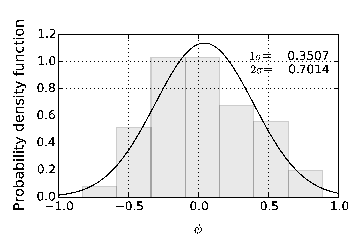
\includegraphics[width=0.6\textwidth]{Chapter4/Figs/MS_latitude_distribution}}
	{\caption{ The gray area shows the probability density function of the parameter $\phi$. The solid black line is the fitted Gaussian distribution. The values standard deviation $1\sigma$ and $2\sigma$ of the normal distribution have been indicated in the top right corner.}\label{ms_dis}}
\end{figure}

\section{Statistical study of longitudinal distribution of MS}
\subsection{Activity maps of active longitudes based on sunspots}

According to \cite{Gyenge2014}, the method highlighted above has been proven and the active longitude was found to be distinct in each hemisphere.
The present investigation started with a similar method as described in \cite{Gyenge2012}. 
In to construct a complete picture of the active longitudes when considering sunspots, the areas and positions of all sunspot groups are included in this analysis.
The solar surface is divided into longitudinal bins of $20^{\circ}$ and the areas of all groups were summed up in each bin: $ A_{i}$ in certain Carrington Rotation between $2097$ and $2128$, the temporal sample over which the MSs locations was recorded.
Next, the longitudinal activity concentration is represented by the quantity $W$ defined by:

\begin{equation}
W_{i,CR} = \frac{A_{i,CR}}{ \sum_{j=1}^{N} A_{j,CR} },
\end{equation}

where $N$ is the number of bins, $\sum_{j=1}^{N} A_{j,CR}$  is the sum of all sunspot groups in a given CR and $A_{i,CR}$ is the  total area of sunspot groups in a Carrington Rotation and at a specific longitudinal bin.

In each Carrington Rotation we omitted all of the $ W_{i,CR}$ values which are lower than the $3\sigma$ significance limit.
The highest peak, inferred as the active longitude in the Carrington Rotation co-ordinate frame, $AL_{CR}$, has been selected from this decayed sample (which contains only the significant peaks) caused by the significance test.
For further analysis, the Carrington longitudes, $\lambda$, will now be transformed, into Carrington phase period: 

\begin{equation}
\psi = \lambda/360^{\circ}.
\end{equation}

Hence, the values of the phases are always smaller or equal (which is the entire circumference) than one. 

The time-variation of the parameter $AL_{CR}$ is plotted in Figure~\ref{AL}.
The vertical axis is the phase parameter, which has been repeated $3$ times.
The northern (left-hand-side) and the southern (right-hand-side) cases are considered separately. Both figures unveil a clear increasing migration pattern. \cite{Usoskin2005,Gyenge2014} found similar patterns at a different time interval. Most of the migration follows a parabola shape (which has been fitted by the least-square method).

\begin{figure}
	\centering
	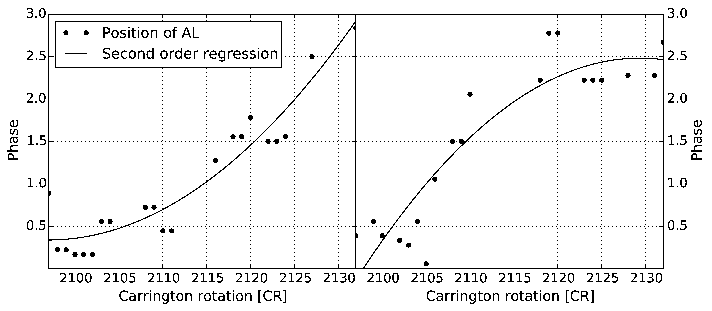
\includegraphics[width=128mm]{Chapter4/Figs/AL}
	\caption{The migration of the active longitudes in the time interval of CR $2097$ to $2128$ based on sunspot groups. The left panel sows the northern hemisphere. The right panel is the southern hemisphere.}
	\label{AL}
\end{figure}

\subsection{Relationship between the AL and MS longitudinal distribution}

\begin{figure}
	\centering
	{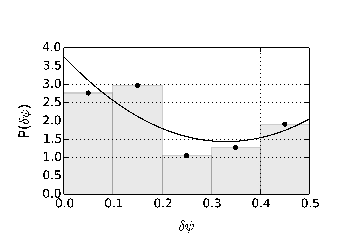
\includegraphics[width=90mm]{Chapter4/Figs/stat}}
	{\caption{Density distribution of the $\delta\psi$ parameter. }\label{stat}}
\end{figure}	

The parameter $\delta\psi$ is now introduced to study the relationship between the active longitude, $AL_{CR}$, defined by sunspot groups, and the longitudinal position of MS $L_{CR}$ in Carrington Rotation co-ordinates. 

\begin{equation}
\delta\psi = \left| AL_{CR} - L_{CR}\right|.
\end{equation}

The parameter $\delta\psi$ has been reduced by a unit phase if it is larger than $0.5$, which means this quantity represents the shortest phase difference between the longitudinal position of a given MS and the position of active longitudes in both hemispheres. 
Next, the $\delta\psi$ samples of the northern and southern hemispheres are now combined. 

The probability density function (PDF) of the quantity $\delta\psi$ is shown in Figure~\ref{stat}. On the $x$-axis the meaning of the lower values reflect on the smallest longitudinal difference in phase, the value $0.5$ phase jumps to the opposite side of the Sun.

The domain of interest of the quantity $\phi$ is $[-1;1]$. 
The $\phi=0$ point contains the northern and southern poles.
The $[0;1]$ sub-domain of $\phi$ represents the northern hemisphere, the ascending $\phi$ values from $0$ to $1$ show the descending latitudes from $90^{\circ}$ to $0^{\circ}$. 
The southern hemispheres have been considered in the same way.

Figure~\ref{ms_dis} shows the result of the statistics above. 
The histogram depicts a normal distribution. 
$\overline{\phi}=0.043$, this implies that most of the MS tend to cluster to the poles

The MS tend to cluster near the active longitudes, which is shown by the first and second peaks: $\delta\psi< 0.2 (<\pm 36^{\circ}$) 61 \% of the candidates.
However, there is a significant peak around $0.5$, which is the signature of the appearance of secondary longitudinal belts. 
The secondary belt exists alongside the primary belt temporally. 
It is always the case that the primary belt is always stronger than the secondary belt, as the name implies), and the phase shift is around $0.5$.
The MS show a similar behaviour, a secondary belt appears for $22\%$ of the events and $\delta\psi< 0.1 (<\pm 18^{\circ}$).

\section{Summary}
We investigated the distribution of MSs detected at the solar surface as function of their longitudinal and latitudinal coordinates in Carrington co-ordinates.

A non-homogeneous latitudinal macrospicule distribution has been found. 
The macrospicules are found to have a non-homogeneous distribution in the Carrington co-ordinate frame.  
Most of the events tend to cluster to the higher latitudes ($95\%$ of MS are with in the $\pm27^{\circ}$ to $\pm90^{\circ}$ heliographical latitude).
The number of the events is found to be growing exponentially from the equator to the pole in both hemispheres. 
A slightly asymmetrical behaviour has been found between the two hemispheres in the studied time interval, where the northern hemisphere was marginally more active than the southern. 

The latitudinal spatial distribution of MS is not uniform either. A large proportion of the MS (83 of from the 101 in our sample) tend to cluster to the AL.
In the case of the primary active longitude belt, the MSs are within $\pm 36^{\circ}$ degrees of the active longitude.
The secondary belt has a $\pm 18^{\circ}$ wide range within which the MSs are found to be concentrated.
This supports the existence of an active longitude at higher latitudes.

A large sample and more comprehensive statistical study is now in preparation for a more detailed search for further identifiable non-homogenous longitudinal distributions of MS in the entire time period covered by observations of the SDO satellite.

% !TeX root = ../thesis.tex
%*****************************************************************************************
%*********************************** Fifth Chapter ***************************************
%*****************************************************************************************


\label{ch:5}
\chapter{A detailed case study of a jet-like feature at the limb}
\begin{pycode}[chapter5]
ch5 = texfigure.Manager(pytex, number=4, base_path='./Chapter5/')
\end{pycode}

\section{Introduction}
Solar jets of various forms are ubiquitous throughout the solar atmosphere, from spicules and macrospicules low in the chromosphere, both of which pass through the transition region, to coronal and X-Ray jets extending into the solar corona \cite{Archontis2008,Majarska2011,Morton2012}. 
Investigations into these phenomena have advanced significantly with recent developments in solar telescope technology, applied on missions like Hinode and the Solar Dynamics Observatory (SDO) and the most recent mission Interface Region Imaging Spectrometer (IRIS).
Features are observed in a range of wavelengths and heights in the atmosphere \cite{Wang1998,Yamaucho2004}. 

Low in the chromosphere the predominant feature is the spicule, these small scale jets are generally found forming over inter-granular lanes and reaching heights of $1$ - $5$ Mm.
They are also very short lived, lifetimes generally only reaching ~$10$ mins.
More importantly there is currently debate as to whether the population of spicules is divided into two forms, Type-1 and Type-2. 
Type-1 are described as longer lived and less explosive with respect to velocity, whereas Type-2 reach higher velocities and higher into the atmosphere, however, are not observed to fall back into the chromosphere \cite{DePontieu2007,Beckers1972,Sterling2000}. 

Having stated this, \cite{Pereira2014} have revealed that Type-2 spicules disappearance may be as a result of heating and moving out of the passband, due to the fact that they are consequently observed in a hotter line which may imply that these features are not in fact separate populations and \cite{Zhang2012} finds no such distinction in population.

Many formation mechanisms have been proposed for spicules, including reconnection, \emph{p}-mode driving and applying accretion disk models in a solar context, for reviews see \cite{Sterling2000} and \cite{Zaqara_Erdelyi2009}.
More recently, the question surrounding spicules is how they effect the atmosphere is particularly pertinent given their vast number. 
Any contribution in terms of solar wind acceleration or heat transfer would be scaled up by their sheer number density.
\cite{Rouppe2015} used coordinated observations with SST and IRIS to study RRE's and RBE's, examining H$\alpha$, Mg II h \& k, C II and Si IV.
The authors find that these spicule-like extensions observed in H$\alpha$ have counter parts in the hotter Magnesium lines and the upper chromosphere/transition region C II and Si IV, which would certainly imply that these features are heating themselves, or the atmosphere around them.
These spicules are similar to other features such as surges, the already mentioned RRB's/RBE's and chromospheric jets, all of which need considering with respect to spicules \cite{Tsiropoula2012, Kuridze2015}.


Higher in the chromosphere, macrospicules are generated, despite their origin laying low in the chromosphere, macrospicules extend through to the transition region and into the corona. 
Larger counterparts of spicules, initially observed in $1975$ by \cite{Bohlin1975} using the Skylab 2 mission using a He $30.4$ nm filter viewing the upper chromopshere.
Bohlin stated their lifetimes to be $5$ to $30$ mins and lengths to be approximately $10$ - $50$ arcsec, and these values have been confirmed \cref{ch:3}

Macrospicules are generally accepted as multi-thermal structures, featuring a cool core and a hot sheath resulting from formation in the cooler atmosphere, from being observed in H$\alpha$ \citep{LaBonte79} and hotter high chromosphere lines such as in \cite{Parenti2002}.
They have also been observed to rotate, \cite{Pike_Mason1998} and \cite{Kamio2010}, the latter paper quotes $-120 \pm 15$kms$^{-1}$ blue shift Doppler velocity on the left side of the macrospicule. 

There are multiple proposals for the mechanism triggering apparent rotation of the macrospicule. 
\cite{Curdt2011} propose that the Sun's differential rotation causes macrospicules rotation, whereas, reconnection events cause the relaxation of a small-scale twisted loop, as demonstrated by \cite{Adams2014}.
Again, with macrospicules extending high into the atmosphere, the question of their effect upon it, is one that needs answering.
\cite{Pike1997} observe outflows from the macrospicule of the order $200$ kms$^{-1}$ in He I and discuss whether these outflows could potentially accelerate the solar wind.
However, work by \cite{Zaqarashvili2014} questions whether jets moving at super-Alfv{\'e}nic speeds might cause a Kelvin-Helmholtz instability to form at the macrospicule/atmosphere boundary, which would, in turn, transport heat into the corona.

A third category of jet-like features, are coronal jets, observed in slightly hotter lines of $17.1$ nm but still visible in EUV, such as those discussed in \cite{Shibata1992} and simulated in \cite{Wyper2016}.
\cite{Shibata1994} propose that these jets are reconnection events, where reconnection is triggered by flux emergence at the base of a small-scale loop.
However, after this initial reconnection, there are several models as to how the system evolves.
\cite{Moore2010} demonstrate a dichotomy in formation mechanism of coronal jets, between the standard 'inverted Y' model by Shibata and the blow-out jet model. 
The blow-out model differs from the standard model due the reconnection leading to a 'curtain' of plasma flow as opposed to the 'spire' from the standard model.
The difference between the two models originates in initial configuration of the overlying arch. 
In standard jets the arch has no appreciable shear, whereas for a blowout jet the arch is twisted and sheared sufficiently to drive the explosive outflow which forms the jet.
Coronal jets have also been shown to accelerate particles into interplanetary space \cite{Li2011} and there is also evidence for repeat onset jets, with several re-occurrences, \cite{Chifor2008} demonstrate repeat on set of jets driven by flux cancellation.

Lastly, we need to consider X-ray jets.
\cite{Shimojo2000} define their physical properties studying 16 separate jet events.
Due to limitations on instrumentation at the time, the authors do not cover the extent of the jets, however, they analyse temperatures, $3 - 8$ MK, and density, $0.4 - 4.0$ cm$^{-9}$.
The authors also discuss flaring at the foot-point of X-ray jets, in that, the temperature is proportional to the size of the initial footpoints.

\cite{Kamio2010} applied a great deal of the background above when studying a macrospicule and X-ray jet forming simultaneously. There is also discussion in \cite{Pike} and \cite{Kim2007} on the appearance of X-ray jets, alongside small scale jets.

In the following sections we comprehensively discuss the physical properties of a case study. In \cref{sec:obs_sect} we present the observations we are using. \ref{sec:time_dist_sect} discusses the evolution of the jet with respect to its extent an the different view of the feature utilising STEREO-A's EUVI. Then move on to a doppler analysis of the jet in \cref{sec:dop_shift_sect}. Lastly, attempt to quantify the effect of the jet on the atmosphere in \cref{sec:temp_map_sect} before making our conclusions.

\begin{pycode}[chapter5]
import numpy as np
import sunpy.map
import matplotlib.pyplot as plt
from mpl_toolkits.axes_grid1 import ImageGrid

onset_path_113 = ch5.data_file('crop_113.npy')
onset_path_114 = ch5.data_file('crop_114.npy')
onset_path_115 = ch5.data_file('crop_115.npy')

ims = [np.load(onset_path_113), np.load(onset_path_114), np.load(onset_path_115)]


multi = texfigure.MultiFigure(1, 3, reference="onset")

for i, anim in enumerate(ims):
    fig = plt.figure(figsize=texfigure.figsize(pytex, scale=0.3, height_ratio=1.3))

    plt.imshow(anim, cmap='sdoaia304', origin='lower')

    Fig1 = ch5.save_figure('onset{}'.format(i+1), fig)
    Fig1.subfig_width = r"0.3\textwidth"
    Fig1.caption = ""
    multi.append(Fig1)

multi.placement = 't!'
multi.caption = "a) Observe the two bright points in the proximity of $(79, 60)$. The point on the left is significantly brighter than the fainter on the right. We emphasise that the brightening around $(60, 50)$ is not a contributor to this jet. b) In this frame the bright points have extended, the fainter point has now extended up to $~95$ and the core of the brighter left feature has grown with it. c) At this point the two separate points are now indistinguishable and the feature is now extending as one column."
\end{pycode}

\py[chapter5]|multi|



\section{Observations}
\label{sec:obs_sect}
We observed a jet-like (hereby referred to as 'the jet') feature at the limb on $21$st June 2016 beginning at $07:30:00$ in CRISP, an instrument installed on the Swedish Solar Telescope (SST) during a period of good seeing, \cite{Scharmer2003}.
We used the H$\alpha$ filter, core line $656.28$ nm with $35$ slit increments from the core covering a $.32$ nm range, $-0.2$ and $+0.12$, further processed using te Multi-Object Multi-Frame Blind Deconvolution (MOMBFD \cite{vanNoort2005}).
The observations were of Active Region 11506 with $xc = 893",\ yc = -250"$ in heliographic coordinates on $930x930$ pixel images, with spatial resolution of $0.012$ arcsec/pixel and temporal resolution of $7.5$ sec.
Due to the constant surveillance under which we have the Sun, we also have simultaneous observations with the Solar Dynamic Observatory (SDO) and the Solar Terrestrial Relations Observatory (STEREO).

Using the Atmospheric Imaging Assembly (AIA), we observe the jet in most of the wavelengths available, $30.4$, $35.5$, $211$, $17.1$ and $13.1$ nm.
AIA on-board SDO (\cite{AIAspec}) provides $4096 \times 4096$ pixel images with a spatial resolution of $0.6$ arcsec per pixel and a cadence of $12$ sec.

Lastly, we also have observations in STEREO using the Extreme Ultra Violet Imager (EUVI) \cite{Defise2001}. 
We are fortunate that when these observations were taken, STEREO A was at approximately $90^\circ$ to the Sun-Earth line, as such we also have observations of this feature as an on-disk feature.
In this case we are using the $30.4$ nm HI instrument, however, the distance from the Earth has now reached a point that the temporal cadence has reduced to $10$ min.
While this is possibly too high to undertake a detailed examination, we can certainly utilise this method to inform us as to the global behaviour of the macrospicule.
As we have a suite of observing instruments to utilise we aim to build a comprehensive description of this feature and how it may affect the environment around it.


\section{Time-Distance Evolution}
\label{sec:time_dist_sect}

Let us begin with the evolution of the jet over time. 
We have utilised a self-built, manual, feature measuring tool, which uses a clicking mechanism to select the foot and tip of the macrospicule, calculates the half height and uses this as a guide to measure the width of the feature.
Using this tool on each frame, and therefore the time cadence of the instrument, we obtain the evolution of the jet and general ballistic information.
We have used this tool on each wavelength to examine the extent upwards through the corona. 
Observations in SDO record the entire lifetime of the feature, however the same is not true for observations using the SST, where the observation window in SST closes at $07:55:00$.

\subsection{Onset}
The jet feature is observed as it forms using SST and, fortunately, we can resolve initial stages of the jet formation.
The jet is observed to initiate in the core of H$\alpha$ with two small bright points forming, and an ensuing jet developing above it. 
\cref{fig:onset} captures the early evolution of the jet in detail.
Evident in \cref{fig:onset1} we find the initial two bright points at the foot of the jet, the bright point of the left being significantly brighter than its countpart on the right.
By \cref{fig:onset2} shows the development of these two points \emph{i.e.} have now become two columns of brighter plasma.
In the final formation stage, \cref{fig:onset3} the jet has formed and is now a distinct feature against the background.
This behaviour is in keeping with the standard jet formation model demonstrated by \cite{Shibata1992}, where the authors describe an 'inverted y' shape of brightened material that is a result of small scale flux emergence reconnection.



\subsection{Evolution}
Let us examine the raw evolution of the jet in the time distance plot in \cref{fig:t-d-plot}.
Here we have utilised the measuring tool to measure the extent of the feature in all the wavelengths in which it is visible.
We find that the overall profile of its evolution contains two distinct peaks in most wavelengths, with the exception of $17.1$ nm.
The first peak comes at $~07:37$ before a decrease in size and subsequent secondary expansion to its maximum length in H$\alpha$ and $30.4$ nm at approximately $07:49$.
This strongly implies that there is a second initialising type event in which a new material is accelerated into the atmosphere.
As such let us turn to the CRISP instrument again.

With its higher resolution, a slit based analysis of the jet can be observed in \cref{fig:sst-slit}.
Notice two distinct curves in the image, the first onset is at approximately $17$ and the second at a bright point originating at $~85$.
We find that in this second phase of the jet, plasma extends higher into the atmosphere.
This result is unusual as previous observations of recurrent jets have shown decay in subsequent initialisation events in observations such as \cite{Jiang2007}.
Unfortunately, a section of material is in front of the base of the jet and obscures our view of the second event.

Considering the observations in multiple wavelengths, we notice the smaller extension visible in the coronal wavelengths.
In these higher temperature lines, the jet appears as a dark line.
Now, this could be due to the fact that the feature is cool and can't be found in the higher temperatures.
However, when examining the jet in AIA $30.4$ nm, the feature appears dark beneath the limb but emissive over it.
It also appears in EUVI $30.4$ m, as a dark feature, therefore we can't assume there is no emission in the higher lines.
This is not unexpected, given its extent in the chromospheric lines, we can to categorise this as a chromospheric feature, as opposed to coronal.

%double check this section
Evidently, the maximum extent of this feature is in SDO $30.4$ and maximises at $12.6$ Mm although the measurements in H$\alpha$ may exceed this were it to be fully visible.
Interestingly, the length of the jet in the coronal lines does not get larger after the second injection on plasma occurs.
This subsequent acceleration of plasma originates from the same location as that of the initial formation, and on the same scale as the first onset.
However, this drives the tip of the jet even higher than the initial tip, measuring the velocity accurately is difficult, due to this acceleration is set against the previous bright material.
An approximation using multiple image steps and using a difference delta produces an average of $46$ kms${^{-1}}$, therefore we can infer that it reaches a higher maximum velocity than the first ejection.

The feature is very thin, averaging $1.13$ Mm in H$\alpha$ and $0.787$ Mm in He II. 
This result is unexpected, it certainly seems to contradict the cool core surrounded by a hot sheath model.
However the errors on the measurement in SDO/AIA recordings are $\pm1.5$ Mm, when taking into account human measurement error and resolution of the instrument.
Where as measurement error on the CRISP/SST images is $\pm0.0885$ Mm, thus, we are more inclined to believe the measurement according to CRISP.
This thin spire is an expected outcome of the standard model of jet formation, more on which later.

\begin{pycode}[chapter5]
import pickle
import def_spic
import def_spic_SST
from matplotlib.dates import DateFormatter

path_131 = ch5.data_file('131_records.pik')
path_171 = ch5.data_file('171_records.pik')
path_211 = ch5.data_file('211_records.pik')
path_304 = ch5.data_file('304_records.pik')
path_335 = ch5.data_file('335_records.pik')
ha_path = ch5.data_file('H_alpha_records.pik')

jet_131 = pickle.load(open(path_131, 'r'))
jet_171 = pickle.load(open(path_171, 'r'))
jet_211 = pickle.load(open(path_211, 'r'))
jet_304 = pickle.load(open(path_304, 'r'))
jet_335 = pickle.load(open(path_335, 'r'))
h_alpha = pickle.load(open(ha_path, 'r'))
obj_131 = jet_131[0]
obj_171 = jet_171[0]
obj_211 = jet_211[0]
obj_304 = jet_304[0]
obj_335 = jet_335[0]
obj_Ha = h_alpha[0]

e_times_131 = obj_131.times
lengths_131 = obj_131.all_length()

e_times_171 = obj_171.times
lengths_171 = obj_171.all_length()

e_times_211 = obj_211.times
lengths_211 = obj_211.all_length()

e_times_304 = obj_304.times
lengths_304 = obj_304.all_length()

e_times_335 = obj_335.times
lengths_335 = obj_335.all_length()

e_times_Ha = obj_Ha.times
lengths_Ha = obj_Ha.all_length()

fig = plt.figure()
plt.plot(e_times_131, lengths_131, color='green', label='13.1 nm')
plt.plot(e_times_171, lengths_171, color='yellow', label='17.1 nm')
plt.plot(e_times_211, lengths_211, color='purple', label='21.1 nm')
plt.plot(e_times_304, lengths_304, color='orange', label='30.4 nm')
plt.plot(e_times_335, lengths_335, color='blue', label='33.5 nm')
plt.plot(e_times_Ha, lengths_Ha, color='darkgoldenrod', label='656.28 nm')
plt.xlabel('Time [UCT]')
plt.ylabel('Length [Mm]')
plt.title('Length of the Jet over time')
fig.autofmt_xdate()

formatter = DateFormatter('%H:%M:%S')
plt.gcf().axes[0].xaxis.set_major_formatter(formatter)

td_fig = ch5.save_figure('t-d-plot', fig)
td_fig.subfig_width = r"\columnwidth"
td_fig.caption = ""
#td_fig.caption = r"Darkgold = H$\alpha$, Blue = 33.5 nm, Orange = 30.4 nm, Purple = 21.1 nm, Yellow = 17.1 nm, Green = 13.1 nm. The CRISP observations end earlier than thewhole evolution of the jet, and the top of the jet is cut off by the top og the image. Therefore we ignore the flatline at the top of the H$\alpha$ line starting at $07:42$"
\end{pycode}

\begin{figure}[t]
	\centering
	\py[chapter5]|td_fig.repr_subfigure()|
	
	\begin{subtable}[b]{0.5\textwidth}
		\centering
		\begin{tabular}{ccc}
		Wavelength, nm & Maximum Length, Mm & Maximum Velocity km/s \\
		656.2 & 11.3 & 0.09 \\
		30.4 & 12.6 & 31.5 \\
		33.5 & 6.0 & 53.6 \\
		21.1 & 5.5 & 50.1 \\
		17.1 & 5.6 & 51.9 \\
		13.1 & 5.6 & 36.6 \\
		\end{tabular}
		\caption{}
	\end{subtable}
	\caption{a) Darkgold = H$\alpha$, Blue = 33.5 nm, Orange = 30.4 nm, Purple = 21.1 nm, Yellow = 17.1 nm, Green = 13.1 nm. The CRISP observations end earlier than the whole evolution of the jet, and the top of the jet is cut off by the top of the image. Therefore we ignore flatline at the top of the H$\alpha$ line starting at 07:42. b) Table of maximised basic spatial properties of the jet.}
\end{figure}


\begin{pycode}[chapter5]
import numpy as np
import sunpy.cm
import matplotlib.pyplot as plt
from astropy.visualization.mpl_normalize import ImageNormalize 
from astropy import visualization

norm=ImageNormalize(stretch=visualization.AsinhStretch(1))

sst_slit_path = ch5.data_file('2016-01-22 14:59:58.507931.npz')

afile = np.load(sst_slit_path)
data = afile['arr_2']

fig = plt.figure(figsize=texfigure.figsize(pytex))
plt.imshow(np.rot90(data[2])[::-1, 100:], cmap='viridis', aspect='auto', origin='lower', norm=norm)
plt.colorbar()
plt.xlabel('Time in SST cadence (7.7 s)')
plt.ylabel('Distance along the slit')
sst_slit_fig = ch5.save_figure('sst-slit', fig)
sst_slit_fig.figure_env_name = r'figure*'
sst_slit_fig.figure_width = r'\columnwidth'
sst_slit_fig.placement = 't'
sst_slit_fig.caption = r'CRISP/SST H$\alpha$ core line slit analysis.'

print(sst_slit_fig.repr_figure(), file=sys.stderr)
\end{pycode}

\py[chapter5]|sst_slit_fig|



\subsection{STEREO-A}
We are fortunate that we can observe the jet feature in the STEREO-A/EUVI, with the position of the spacecraft at approximately $90^\circ$ to the Sun-Earth line.
This facilitates the building of a larger picture of the behaviour of the jet, the downside to this however, is that with STEREO-A being at such a distance the cadence is low, $~10$ mins.
In this case we obtain 4 images in $30.4$ nm in which the jet is observed.
The jet appears as a dark fibril like feature originating at ***A POINT IN SPACE*** and extending across the disk to a length of $45.1$arcsec.
Significantly, the component of extension in the East-West direction is not insignificant, approximately $30$ arcsec.
With this information we calculate that the total length of the feature, taking into account both SDO and STEREO's view, is $25.5$ Mm.



\begin{pycode}[chapter5]
import numpy as np
import sunpy.map
import matplotlib.pyplot as plt
import astropy.units as u
from glob import glob
from mpl_toolkits.axes_grid1 import ImageGrid

path_stereo_1 = ch5.data_file('20120621_072615_n4eua.fts')
path_stereo_2 = ch5.data_file('20120621_073615_n4eua.fts')
path_stereo_3 = ch5.data_file('20120621_074615_n4eua.fts')
path_stereo_4 = ch5.data_file('20120621_075615_n4eua.fts')

stereos = [path_stereo_1, path_stereo_2, path_stereo_3, path_stereo_4]


multi_ST = texfigure.MultiFigure(2, 2, reference="stereo")


for i, im in enumerate(stereos):
	fig = plt.figure(figsize=texfigure.figsize(pytex, scale=0.4))
	
	amap = sunpy.map.Map(im)
	crop = amap.submap([-640, -510]*u.arcsec, [-430, -330]*u.arcsec)
	crop.plot(title=False)
	Fig1 = ch5.save_figure('stereo{}'.format(i+1), fig)
	Fig1.subfig_width = r"0.4\textwidth"
	Fig1.caption = ""
	multi_ST.append(Fig1)

multi_ST.placement = 't'
multi_ST.caption = "EUVI $30.4$ nm images from STEREO on $21$st June at a) $07:26:15$, b) $07:36:15$, c) $07:46:15$ and d) $07:56:15$. "
\end{pycode}

\py[chapter5]|multi_ST|



\section{Doppler shift}
\label{sec:dop_shift_sect}

Possibly the most valuable information to be gained about the development of jets, is pertaining to it rotational behaviour, therefore, we will use the spectral increments from the CRISP instrument to obtain line-of-sight Doppler velocities.
There is, however, a hindrance with this.
There are two seperate forms of the emmission spectra within the image.
The region where the jet initialises, is on disk, and as a result the spectral analysis reveals an absorption spectra.

\subsection{MCMC Method}

We have developed this algorithm to address this particular problem, using the overall shift of the emission line from the standard emission. 
Over the limb, however, the spectral profile changes to emission and we find two peaks.
As a consequence of this, finding the total shift away from the core, $656.28$ nm, is made more complex.
For pixel points which are on-disk, we fit a single Gaussian and calculate the minima, as is standard, and for the two peak spectra, we have utilised a double Gaussian, finding the minima between the two.
However, the problem becomes evident when we need to change between the two routines.

We have utilised a Markov Chain Monte Carlo (MCMC) (\cite{Richey2010}) method to find the most accurate fit and the Bayesian Information Criterion (BIC) to test which of the two fits is most appropriate from a given line as a solution to this problem.

This method takes the 35 spectral intensity for a given pixel and samples multiple possible fits for the profile these produce.
We then find the most likely fit from this range and minimise this final fit to find the mean value of the fit.
Difference between the original core value and mean of the new fit is the calculated shift in wavelength, and therefore, the line-of-sight velocity for the chromospheric plasma.
The process is the same for both single and double Gaussian fitting and as such we apply a BIC to test which fit is more appropriate.
BIC has limitations when the number of parameters is of the same order of the size of the sample and differentiating between multiple complex models.
In this case the sample is larger than the number of parameters and we are only testing two possible models, as such, we can use the test with confidence in the results.

The result of applying the above method to the CRISP/SST spectroscopic dataset is presented in \cref{fig:dop-exam}.
Immediately apparent, is the banding structured red and blue shifts, the effect is created as a result of the optical depth created when observing at the limb. 
The jet forms in amongst a blue band of smaller thin structures, making early observations in the dopplergrams difficult.  

\subsection{Analysis}
This particular feature, as has already been mentioned, has two events in which material is accelerated upwards into the solar atmosphere.
The first event is not readily visible in the dopplergrams, difficult as it is to pick out against a line of spicule-like features all showing blueshifts, towards the viewewing direction.
This result is to be expected given the we have demonstrated movement away from the 'camera' in \cref{fig:stereo}.
Whereas, the second expulsion of material, originating at $07:37$, exhibits the classic behaviour of a rotating feature in dopplergrams, a red/blue split over the body of the feature. 
 
It is clear that the second event comes from a similarly small element to the first and evolves upwards, joining the full formation of the jet, hence why the apparent rotation of the jet does not appear to spread across the rest of the jet as seen in H$\alpha$.

As the jet evolves we see an initial blue shift, matching the acceleration upwards seen in H$\alpha$, and it is only after a few second seconds of evolution that rotational behaviour begins to become evident.
The first panel in \cref{fig:dop-exam} at $07:37:44$ demonstrates the first panel where there might be in inkling of redshift on the right ride of the feature, with a thin line registering as moving away from the camera.
Noticeably, this rotation does not begin at the base of the feature, instead, the rotation manifests from the tip downwards over the next two images at $07:37:51$ and $07:37:59$.

By the time the jet reaches $07:39:07$, we begin to observe a thin formation of red shift at the right side of the base of the feature, and by $07:38:15$, the red-shift has entirely taken over the right hand side.
Though once again, the next frame shows progression up the spire of the feature.

We subsequently observe the sift to disappear from the right hand side of the jet, however, the subsequent two images show an element of red shift now on the left of the feature.
This element consequently develops into longer feature in $07:38:53$ and subsequent images, to the point where red shift now dominates the left hand side of the feature.

This is a result of the magnetic pressure acting as restoring force, and rotating the feature in the opposite direction. 
However in this case, not to the same magnitude, an expected outcome due to inherent loss of energy from the system.
By the last panel at $07:39:16$, the feature has returned to a 'neutral' state, as such we can estimate an approximate period of a minute and a half.

This behaviour is extremely interesting as it demonstrates a torsional motion of the entire body of the feature, with the structure rotating anti-clockwise and then clockwise.
This is a result of the release of magnetic tension in the initial reconnection event causing an unwinding of the inherent twist in the initial loop.
We suggest that, as a result of the speed of the initial acceleration of the plasma material, this untwisting began at the top of the plasma column as is seen in $07:37:51$.
The peak of this untwisting, when the red shift dominates the RHS at $07:38:15$, with the highest velocity values observed at approximately $3-4$ kms${^{-1}}$ and the 'body' of the feature demonstrating velocities in the range $1.0-1.5$ kms${^{-1}}$.

The velocity values given here are slow compared to those presented in previous works, however, we believe these to be accurate, and attribute this to the smalls scale of the initial loop.
A larger scale loop would mean that the magnetic tension would be greater, and hence, experience greater restoring force, inducing higher velocities.

  




\begin{pycode}[chapter5]
import sunpy
import slit

import matplotlib as mpl
import matplotlib.pyplot as plt
from matplotlib import colors
from mpl_toolkits.axes_grid1 import ImageGrid
from matplotlib import gridspec
from matplotlib.collections import LineCollection

import numpy as np
import numpy.ma as ma

import astropy.units as u
import datetime
from datetime import timedelta
from astropy.constants import c
from sunkitsst.read_cubes import read_cubes
from glob import glob

# some funcitons
def get_time(ind, time_0):
    current_time = time_0 + timedelta(seconds=7.7)*ind
    return current_time

def truncate_colormap(cmap, minval=0.0, maxval=1.0, n=100):
    new_cmap = colors.LinearSegmentedColormap.from_list(
        'trunc({n},{a:.2f},{b:.2f})'.format(n=cmap.name, a=minval, b=maxval),
        cmap(np.linspace(minval, maxval, n)))
    return new_cmap


#dop_frames = [76,77,78,79,80,81,82,83,85]
dop_frames = [76,77,78,79,80,81,82,83,85,86,87,88,89]
frame_numbers = np.arange(75,90)

# read in some datas
dop_files = []
for i in frame_numbers:
    dop_files.append(ch5.data_file('dops/dop_arr_test0{}.npy'.format(i)))
dop_files.sort()

t0_ha = datetime.datetime(2012,6,21,7,15,9)
t0_dop = get_time(100, t0_ha)

dops = np.zeros((len(dop_files), 331, 120))
for i, afile in enumerate(dop_files):
    dops[i] = np.load(afile)

# process the the dops to get vels
l0 = 6562.8*u.Angstrom
dops = dops*u.Angstrom
dops = (l0-dops)/l0*c
dops = dops.to(u.km/u.s)

# get the variables for the slit analysis
# lets use a perfectly horizontal slit
x1 = 45
x2 = 65
y1 = y2 = 130
N = 0


### make the graph for time and slit
slit_inds = slit.slit_count(x1, y1, x2, y2, 0, 0, N)

# index the arrays properly
inds_x = np.array([slit_inds[:,:,0]])
inds_y = np.array([slit_inds[:,:,1]])
ind_dop = dops[:,inds_y, inds_x]

dop_fin = ind_dop[:,0]

# get the dopplergrams associated with the rotation
slit_list = []
for i, n in enumerate(frame_numbers):
    temp = dop_fin[i]
    temp[temp > 20*dop_fin.unit] = np.NaN
    slit_list.append(temp)

xy_slit = [np.array(zip(range(len(slit_inds[0])), s[0].value)) for s in slit_list]


n_cmap = truncate_colormap(plt.get_cmap('Oranges'), 0.3, 1.0)


# new figure using subplot2grid specificially
fig = plt.figure(figsize=texfigure.figsize(pytex, height_ratio=1.3))
gs = gridspec.GridSpec(3,8)
ax1 = plt.subplot(gs[0,0:2])
ax2 = plt.subplot(gs[0,2:4])
ax3 = plt.subplot(gs[0,4:6])
ax4 = plt.subplot(gs[0,6:8])
ax5 = plt.subplot(gs[1,0:2])
ax6 = plt.subplot(gs[1,2:4])
ax7 = plt.subplot(gs[1,4:6])
ax8 = plt.subplot(gs[1,6:8])
ax9 = plt.subplot(gs[2,0:2])
ax10 = plt.subplot(gs[2,2:4])
ax11 = plt.subplot(gs[2,4:6])
ax12 = plt.subplot(gs[2,6:8])
 
ax_list = [ax1, ax2, ax3, ax4, ax5, ax6,
           ax7, ax8, ax9, ax10, ax11, ax12]

for n, an_ax in zip(dop_frames, ax_list):
    i = np.where(frame_numbers == n)[0][0]
    time_dop = get_time(n, t0_dop).strftime('%H:%M:%S')
    temp_dop = dops[i].value
    y_shift = 40
    im = an_ax.imshow(temp_dop[:250,40:], vmax=15, vmin=-15,
                      cmap='RdBu_r', origin='lower',
                      norm=mpl.colors.SymLogNorm(1),
                      interpolation='none')
    an_ax.plot([x1, x2], [y2-y_shift,y2-y_shift], color='k')
    an_ax.set_title('{}'.format(time_dop), fontsize=10)
    an_ax.set_xlim(left=1, right=80)
    an_ax.set_ylim(bottom=1, top=225)
    an_ax.locator_params(axis='x', nbins=4)
    im.cmap.set_under('w')
    im.cmap.set_over('w')

cb = fig.colorbar(im, ax=ax9, pad=0.1)
cb.set_label('Velocity {}'.format(dop_fin.unit._repr_latex_()))
cb.set_ticks([-15,-9,-6,-3,-2,-1,0,1,2,3,6,9,15])

# line collection section
n_cmap = truncate_colormap(plt.get_cmap('Oranges'), 0.3, 1.0)

# fig, ax = plt.subplots()
line_segments = LineCollection(xy_slit,
                               linewidths = 0.5,
                               linestyle='solid',
                               cmap=n_cmap)

line_segments.set_array(np.arange(1,len(slit_list)+1))
#ax10.add_collection(line_segments)
#ax10.axis([1,xy_slit[0].shape[0]-1,-1.6,1.6])
#ax10.axhline(0, color='k', linewidth=0.5)

#axcb = fig.colorbar(line_segments)
#axcb.set_label('Frame Number')
#axcb.set_ticks(range(1, len(xy_slit)+1))
#ax10.set_title('Slit across')
#ax10.set_xlabel('Distance Along Slit [pixels]')
#ax10.set_ylabel('Velocity {}'.format(dop_fin.unit._repr_latex_()))
#plt.sci(line_segments)

gs.tight_layout(fig, w_pad=0.2, pad=4)

dop_grid = ch5.save_figure('dop-exam', fig)
dop_grid.figure_width = r'\textwidth'
dop_grid.placement = 't'
dop_grid.caption = 'Above is the result of the dopplergram processing during the evolution of the second ejection of plasma starting at $07:37:00$'


\end{pycode}

\py[chapter5]|dop_grid|





\section{Effect on the atmosphere}
\label{sec:temp_map_sect}

With the increased resolution we can visually inspect the boundary between the jet and atmosphere.
\cref{fig:demo-bound} details the evolution of the jet in the core of H$\alpha$ in over $115$ seconds.
At the boundary we observe narrow dark columns in the emission on either side of the jet.
Given that they appear on either side of the jet column and that the observations are in the core of the $H\alpha$ line, it is unlikely that this would be caused by a doppler-like effect.
One possibility is that the cause is an instability effect, such as shear or Kelvin-Helmholtz, seen in \cite{Zaqarashvili2014} as the jet moves throughout the higher atmosphere.
Supporting this hypothesis is that these images were recorded in the 'second phase' of the jet \emph{i.e.} after the second reconnection and the jet extends to its peak in $30.4$ nm. 
As such, it is possible that these columns are a result of plasma being accelerated through the less dense atmosphere.

One of the possible primary results of these instabilities is a dissipation of energy into the surrounding atmosphere, as such we might expect an increase in temperature of the surrounding atmosphere.
To this end we will utilise the temperature calculation method highlighted in \cite{Leonard2014}.

The authors use a Differential Emission Measure (DEM) to obtain a temperature response from the SDO/AIA measurements.
The temperature response is a combination of the wavelength response from the instrument and the contribution function which describes the emission from a given temperature.
When using such a scheme, we need to decide on a general DEM profile to be applied to all pixels.
The method uses a Gaussian scan across the emission in each line and property of the Gaussian; mean, amplitude and width. 
Utilising a narrow Gaussian seems to provide the most accurate values when compared to synthetic observations.

\cref{fig:temp-slit} demonstrates the behavioural change of the temperature across the normal of the feature by slit based analysis.
By performing this analysis over the time domain of the second ejection of plasma material, we will acertain whether the feature has any impact on the atmosphere.
The difficulty with this form if measurement is that the feature itself is not particularly wide, $~1$ Mm, and therefore is has only one or two pixels of actual jet material for us to examine.
The jet is located around the $3rd$ and $4th$ pixels of the x axis, and as we would expect we see a moderate dip, when compared to the surroundings. 
Noticeable as well, however, is that at what is approximately the boundaries, there is a peak in temperature, before it drops as distance increases with respect to the jet.

These values are not conclusive, we require temperature maps on a much finer spatial scale, and as well, new techniques to develop to overcome the problems of the extremely broad H$\alpha$ and He II lines causing a blurring of possible values.
However, in conjunction with the observations presented here of possible shearing or Kelvin Helmholtz instability causing a lack of emission at the boundary of the jet, we can present the hypothesis more confidently.
In terms of the bigger picture in which spicules/jets/macrospicules contribute to heating of the solar corona, the results produced by this feature are not typical.
With respect to other studies, this feature cannot be considered that quick, or large, or excessively rotational, yet it may be having a measurable effect.
Hence, applying this kind of comprehensive analysis to multiple jets, particularly rapidly evolving examples, to ascertain their impact on the atmosphere fully is the next area of investigation for these jets.
An endeavour which will be aided significantly by the operation commencement of DKIST, with its superior everything.
 


\begin{pycode}[chapter5]
import numpy as np
from glob import glob
import sunpy.map
import matplotlib.pyplot as plt

im_1 = ch5.data_file('core_Ha_dark_165.npy')
im_2 = ch5.data_file('core_Ha_dark_170.npy')
im_3 = ch5.data_file('core_Ha_dark_175.npy')
im_4 = ch5.data_file('core_Ha_dark_180.npy')

ims = [im_1, im_2, im_3, im_4]

multi_db = texfigure.MultiFigure(1, 4, reference="demo-bound")
multi_db.caption = "Sequence of images detailing an intermediate phase of the jets evolution. Beggining with a) 07:36:19, b) 07:36:19, c) 07:37:36 and d) 07:38:15"
for i, im in enumerate(ims):
	fig = plt.figure(figsize=texfigure.figsize(pytex, scale=0.25, height_ratio=1.3))
	ax = plt.gca()
	ax.tick_params(axis='both', colors='white', labelcolor='black')
	afile = np.load(im)
	val_max = np.max(afile)
	plt.imshow(afile, cmap='Greys_r', vmin=0.16*val_max, vmax=val_max, origin='lower', interpolation='none')
	Fig1 = ch5.save_figure('demo_bound{}'.format(i+1), fig)
	Fig1.subfig_width = r"0.2\textwidth"
	Fig1.caption = ""
	multi_db.append(Fig1)

\end{pycode}

\begin{pycode}[chapter5]
import numpy as np
import matplotlib.pyplot as plt
from matplotlib.collections import LineCollection
from matplotlib import colors

import sunpy.map
import slit

from astropy.io import fits
import astropy.units as u

from glob import glob

files = glob('/storage2/temperature_maps/data/full_gauss/*.fits')
files.sort()

def proc_file(x):
    with fits.open(x, memmap=True) as f:
        data = f[0].data[..., 0]
        header = dict(f[0].header)
        m = sunpy.map.Map((data, header))
        m.plotsettings = {'cmap':'coolwarm'}
        crop = m.submap((857.9, 957.94)*u.arcsec,
                 (-197.92, -297.92)*u.arcsec)
    return crop 


submaps = []
for afile in files[28:40]:
    temp = proc_file(afile)
    submaps.append(temp)

mc = sunpy.map.Map(submaps, cube=True)


image_1 = slit.slit(mc, [909, 911]*u.arcsec, [-245, -242]*u.arcsec, 1, -1, +1)

temp_values = image_1[0]
temp_inds = image_1[1]


xy_slit = [np.array(zip(range(len(temp_inds)), temp_values[0,:,i])) for i in range(temp_values.shape[2])]

def truncate_colormap(cmap, minval=0.0, maxval=1.0, n=100):
    new_cmap = colors.LinearSegmentedColormap.from_list(
        'trunc({n},{a:.2f},{b:.2f})'.format(n=cmap.name, a=minval, b=maxval),
        cmap(np.linspace(minval, maxval, n)))
    return new_cmap

nmap = truncate_colormap(plt.get_cmap('Oranges'), 0.3, 1.0)

line_segments = LineCollection(xy_slit,
                               linewidths=0.25,
                               linestyle='solid',
                               cmap=nmap)

line_segments.set_array(np.arange(len(temp_values[0,0,:])))

fig, ax = plt.subplots(figsize=texfigure.figsize(pytex))


ax.add_collection(line_segments)
ax_cb = fig.colorbar(line_segments)
ax_cb.set_label('Time')
ax.axis([0,5 , 6.4, 6.6])
ax.set_title('Temperature over slit')
ax.set_xlabel('Distance across slit')
ax.set_ylabel('Temperature')
plt.sci(line_segments)
plt.draw()

temp_slit = ch5.save_figure('temp-slit', fig)
temp_slit.caption = "The AIA maps were processed into temperature maps, and a slit was taken at the half height, perpendicular to the axis of evolution. The temperature maps were taken for the time over which the second acceleration of material occured. The colorbar indicates the passage of time and the various lines applicable to the slits is demonstrated."


\end{pycode}

\py[chapter5]|multi_db|

\py[chapter5]|temp_slit|

\section{Discussion \& Conclusion}
\label{sec:DandC}

We observe a jet-like feature at the solar limb on $21$st June 2012 at $07:30:00$ on the solar limb, centred at $910$, $234$ solar x and y.
We have multiple methods with which to view the feature, CRISPT/SST, the range of AIA/SDO coronal wavelengths and SECCHI/STEREO-A.
We have utilised multiple analysis techniques to build a comprehensive picture of the jet-like features motion and the possible impacts on the atmosphere above it.

From the observation of this feature, we can draw the following conclusions
\begin{itemize}
	\item{This particular feature is visible in H$\alpha$ and He II $30.4$, and thus, is inherently a chromospheric object.}
	\item{The jet has two separate ejections of material. Reaching a maximum \emph{length} of $25$ Mm}
	\item{The formation of the jet is observed to be similar to the standard jet formation mechanism.}
	\item{The jet has a rotational component to its motion}
\end{itemize}

The feature is observed to extend to $12.6$ Mm in He II $30.4$ nm (and is only found to be shorter in H$\alpha$ due to moving out of the viewing field of view).
Its lifetime is measured of to be $20$ mins and radial velocities are found to be maximised during the initial acceleration, and are of the order $50 - 60$ km$s^{-1}$ during the first acceleration of the feature.
However the second acceleration of material proves awkward to measure accurately, however we estimate slightly higher maximum velocities, but similar averages over the extension upwards. 
This very much puts this feature in the category of macrospicules, agreeing with the values presented in \cref{ch:3}.

However the feature exhibits similar formation mechanisms as a standard jet following the pattern demonstrated in \cite{Shibata1992} and then built on by \cite{Moore2010}, who also presented the blowout jet mechanism.
With the two visible bright points in the H$\alpha$ images which come to form an, all be it, long thin bright arch before forming the characteristic spire of a the standard jet.
Unfortunatley, Hinode's XRT instrument was in a power down mode during the formation of this feature and RHESSI did not record the event, as such, we are missing crucial X-ray data.

If an increase in the X-ray radiation were to be found, the question as to the categorisation of such a feature becomes important.
Given that we observe several of the key indicators of a standard jet, could this not also be classified as a standard jet? 
Inspite of this features relatively small size, this could be classified as an X-ray jet.
However the question remains, is this a macrospicule?
And if so, do we classify the feature as a macrospicule or a standard jet?

One possible differentiator is the appearance in the higher coronal wavelengths.
In this case, the jet appears as an absorption feature, against the brighter limb.
This does not mean that the jet does not reach coronal temperatures, in $30.4$ nm the jet appears as absorption below the limb and as emission above it.
We cannot conclusively say that the jet contributes to the coronal emission by visual inspection.

Therefore, we propose that this is a standard jet, and as a community, we need to fully address the underlying physics of macrospicules.
This is despite the ambiguity about its appearance in the coronal emission lines, but the underlying physics is enough to draw this conclusion.

The spectroscopic readings, as show in \cref{dop_shift_sect}, demonstrates a small, but appreciable perturbation in the rotational velocity of the jet like feature.
We find that the jet exhibits a torsional behaviour, demonstrating shifts indicating rotation in one direction and then the other.
The magnitude of these velocities is, however, low.
we conclude that this is a result of the very small source loop of the feature, although this of course needs further enquiry. 

With respect to the features affect on the atmosphere, we find a boundary interaction between the jet and atmosphere in the H$\alpha$ images.
This interaction has manifested as dark streaks at the every edges of the feature during the same phase in which the second event causes the acceleration of further plasma.
It is also the phase in which we observe the torsional rotation of the jet.
Whether these dark streaks are physically significant we cannot comment upon too confidently at this time, but they appear at the same time as the second acceleration and the onset of rotational behaviour, cannot merely be coincidence.

% !TeX root = ../thesis.tex
%*****************************************************************************************
%*********************************** Conclusion ***************************************
%*****************************************************************************************

\label{ch:conc}
\chapter{Conclusions}

Macrospicules are an intriguing feature of the solar atmosphere.
The work that is presented in this thesis has attempted to shed some light on these prevalent parts of the atmosphere.
\cref{ch:3} can be easily compared to the previous works on a like-for-like basis.
The previous examples of measurements, given by \cite{Bohlin1975} and \cite{Dere89}, are compared in \cref{table:final-properties}.
The values found here compare particularly well with Bohlin, however, the work by Dere finds more conservative values.
Given the improved nature of instrumentation and measuring tools utilised in this work, we assert that the values found here should become the new expected measurements defining a macrospicule.

This study also found no divergence in the population of features measured.
Such an effect could be expected were MS very similar to another feature, but with separate underlying physics.
Of course, the possibility remains that, they are part of a larger scale feature, such as X-Ray jets, which, has been discussed on multiple occasions, \cite{Parenti2002, Kamio2010}.
In these cases, the jet-like features' properties are similar to those of regular MS, but there is no evidence to support this hypothesis within this study.   

With respect to the ballistics and energetics of the feature, we find the unexpected effect of a macrospicule becoming thinner as it falls down in the atmosphere.
Another theory could be that the magnetic pressure would cause the width to increase, however the evidence does not agree with this, as such we need to think about the macrospicule not just as a column of regular plasma.
The likely case is that the plasma begins to flow down the magnetic field lines, in a similar manner to evanescence, resulting in a decrease in the width of the feature.

\cref{ch:4} demonstrates that macrospicules' properties are dictated by larger processes in the Sun.
That macrospicules tend to form along an active longitude is likely due to the influence of the tachocline.
This result has subsequently been given more credence as a result of the work undertaken by \cite{Kiss2017} finding a short term, $1$ - $2$ year cycle in macrospicule length.
Again, this could be due to the influence of the tachocline dynamo effects creating the global magnetic field.

\cref{ch:5} presents the most comprehensive view of a macrospicule in this thesis.
The most significant result, is demonstrated very clearly in the line of sight dopplergrams.
The macrospicule feature clearly shows a rotation initially in the anti-clockwise direction, before slowing in rotation rate, stopping and then rotating clockwise.
This is the first observation of such behaviour in a macrospicule.
In contrast, there have been multiple observations and simulations of rotating jet-like features, e.g. \cite{Kamio2010, Curdt2011, Majarska2011}, however, this is the first work demonstrating torsional oscillating motion in either jet or macrospicules.
It is also apparent that the observed `unwinding' motion starts from the tip of the macrospicule before moving downwards.  
This unequivocally proves that MS have an intrinsic magnetic field.
The presence of a magnetic field in the macrospicule constrains the formation mechanism, to those involving the simultaneous expulsion of plasma and magnetic field, which is highlighted in \cref{sec:recon}.

The resolution of SST allows us to examine the footpoint of the macrospicule.
The conclusion that arises from this is that the macrospicule seems to undergo a formation event similar to the \cite{Shibata1992} standard jet formation model.
The brightenings evident in the H$\alpha$ line, show two much smaller brightpoints evolving and joining before the spire eventually forms.
The extension of this feature in the lower temperature emission lines, where it extends the furthest, is roughly $12$ Mm.
We have therefore observed a small-scale feature with a very similar formation mechanism to larger coronal jets.
This leads to the conclusion that macrospicules should perhaps be classified as standard jets.
Given that this feature is very thin, but \cref{ch:3} shows average widths of the order of $7$ Mm, therefore should the population be separated in terms of formation processes, i.e. standard and `blowout' style MS, in the same way as jets?

Macrospicules and their relationship (or lack thereof) with jets, will continue to be essential to our understanding of the solar atmosphere, given that they originate in the low chromosphere and extend up into the corona.
The questions of the most importance at the moment are of their structure and formation mechanism.
Both of these may be answered by the new DKIST telescope.
The leap forward that DKIST will take with respect to spatial and temporal resolution will allow us to examine the footpoints of these features with significantly greater accuracy.
Possibly more intriguing is the body of MS themselves.
Given the `unwinding' of magnetic twist observed in \cref{ch:5}, it may be possible to inspect individual strands of flux rope, which could answer:

\begin{itemize}
	\item{Are the MS unwinding in all cases?}
	\item{Could the twisting motion be a result of a driver from below?}
	\item{Do the MS always have a torsional or helical component?}
	\item{Can MS be considered as a major factor with respect to heating or solar wind acceleration?}
\end{itemize}
 
 
Those are just the questions considering MS on their own.
Macrospicules' current place in the plethora of jet-like solar features is still far from clear, despite this work.
Are MS instances of multiple spicules `superposing' and becoming a much larger feature as supposed by \cite{Xia2005}?
Are they the cool component of X-Ray jets as in \cite{Parenti2002}? In which case should we merely be calling them X-Ray jets observed in chromospheric emission lines?
There has been much work on the subject of H$\alpha$ and He II $30.4$ nm MS, including work by \cite{LaBonte79,Wang1998} but we have yet to conclusively prove that these features are one and the same.
However, \cref{ch:5}, again demonstrates that this is the case.
 
The future of the study of macrospicules lies with observations.
At the moment, there is no shortage of models sufficiently complex to describe, in detail, the method by which macrospicules are formed, authors such as \cite{Murawski2011}, \cite{Archontis2005} and \cite{Moreno2008} have covered his extensively.
What is required is tuning of the initial conditions and magnetic configuration at the time of onset.

This is now possible with the building of DKIST.
DKIST will be the most advanced telescope of the current age of solar observations, with a 4 meter mirror able to resolve $10$ km on the solar surface and a very high temporal cadence, it can be pushed as low as $1/3$ of a second [\cite{Woeger2016}].
With this instrument, we will be able to record the moment that a macrospicule is formed in extreme detail.
The most efficient way, given macrospicules infrequency compared to spicules, would be to focus attention to the coronal hole boundaries given that $20\%$ of macrospiules are formed there, \cref{ch:3}, and the area too cover is much smaller than the alternative coronal holes and quiet Sun.

Over a large sample window, collecting as many macrospicules evolution as possible, would allow a statistical distribution of the rotational velocities of the macrospicules to be found.
Testing whether the rotational velocity measured in \cref{ch:5} is the expected value or overly slow.
This will have an impact going forward as it would demonstrate whether the Kelvin-Helmholtz instability [\cite{Zaqarashvili2014}] could heat the corona through the volume of spicules/macrospicules in the chromosphere. 

However, the most import subject with respect to macrospicules is their classification among the solar jets. 
\cref{ch:5} demonstrates that a feature with similar size and dimension to those in \cref{ch:3} can have formation patterns equatable to much larger features such as X-Ray and EUV jets.
As the study of jets carries forward, the question at the front the solar physicist's mind should be, are jets observed in the lower temperatures actually different features to hotter jets, or just their footprint lower in the atmosphere?


 




% ********************************** Back Matter *******************************
% Backmatter should be commented out, if you are using appendices after References
%\backmatter

% ********************************** Bibliography ******************************
\begin{spacing}{1.1}

% To use the conventional natbib style referencing
% Bibliography style previews: http://nodonn.tipido.net/bibstyle.php
% Reference styles: http://sites.stat.psu.edu/~surajit/present/bib.htm

\bibliographystyle{apalike}
%\bibliographystyle{natbib} % use this to have URLs listed in References
\cleardoublepage
\bibliography{References/references} % Path to your References.bib file
\newcommand*\aap{A\&A}
\let\astap=\aap
\newcommand*\aapr{A\&A~Rev.}
\newcommand*\aaps{A\&AS}
\newcommand*\actaa{Acta Astron.}
\newcommand*\aj{AJ}
\newcommand*\ao{Appl.~Opt.}
\let\applopt\ao
\newcommand*\apj{ApJ}
\newcommand*\apjl{ApJ}
\let\apjlett\apjl
\newcommand*\apjs{ApJS}
\let\apjsupp\apjs
\newcommand*\aplett{Astrophys.~Lett.}
\newcommand*\apspr{Astrophys.~Space~Phys.~Res.}
\newcommand*\apss{Ap\&SS}
\newcommand*\araa{ARA\&A}
\newcommand*\azh{AZh}
\newcommand*\baas{BAAS}
\newcommand*\bac{Bull. astr. Inst. Czechosl.}
\newcommand*\bain{Bull.~Astron.~Inst.~Netherlands}
\newcommand*\caa{Chinese Astron. Astrophys.}
\newcommand*\cjaa{Chinese J. Astron. Astrophys.}
\newcommand*\fcp{Fund.~Cosmic~Phys.}
\newcommand*\gca{Geochim.~Cosmochim.~Acta}
\newcommand*\grl{Geophys.~Res.~Lett.}
\newcommand*\iaucirc{IAU~Circ.}
\newcommand*\icarus{Icarus}
\newcommand*\jcap{J. Cosmology Astropart. Phys.}
\newcommand*\jcp{J.~Chem.~Phys.}
\newcommand*\jgr{J.~Geophys.~Res.}
\newcommand*\jqsrt{J.~Quant.~Spec.~Radiat.~Transf.}
\newcommand*\jrasc{JRASC}
\newcommand*\memras{MmRAS}
\newcommand*\memsai{Mem.~Soc.~Astron.~Italiana}
\newcommand*\mnras{MNRAS}
\newcommand*\na{New A}
\newcommand*\nar{New A Rev.}
\newcommand*\nat{Nature}
\newcommand*\nphysa{Nucl.~Phys.~A}
\newcommand*\pasa{PASA}
\newcommand*\pasj{PASJ}
\newcommand*\pasp{PASP}
\newcommand*\physrep{Phys.~Rep.}
\newcommand*\physscr{Phys.~Scr}
\newcommand*\planss{Planet.~Space~Sci.}
\newcommand*\pra{Phys.~Rev.~A}
\newcommand*\prb{Phys.~Rev.~B}
\newcommand*\prc{Phys.~Rev.~C}
\newcommand*\prd{Phys.~Rev.~D}
\newcommand*\pre{Phys.~Rev.~E}
\newcommand*\prl{Phys.~Rev.~Lett.}
\newcommand*\procspie{Proc.~SPIE}
\newcommand*\qjras{QJRAS}
\newcommand*\rmxaa{Rev. Mexicana Astron. Astrofis.}
\newcommand*\skytel{S\&T}
\newcommand*\solphys{Sol.~Phys.}
\newcommand*\sovast{Soviet~Ast.}
\newcommand*\ssr{Space~Sci.~Rev.}
\newcommand*\zap{ZAp}

% If you would like to use BibLaTeX for your references, pass `custombib' as
% an option in the document class. The location of 'reference.bib' should be
% specified in the preamble.tex file in the custombib section.
% Comment out the lines related to natbib above and uncomment the following line.

% \printbibliography[heading=bibintoc, title={References}]


\end{spacing}

% ********************************** Appendices ********************************

\begin{appendices} % Using appendices environment for more functunality

%\include{Appendix1/appendix1}

\end{appendices}

% *************************************** Index ********************************
\printthesisindex % If index is present

\end{document}
